\chapter{Monte Carlo Synthetic Acceleration Methods for the $SP_N$ Equations}
\label{ch:spn_equations}

The neutron transport problem is complicated. Solutions cover a large
phase space and the problems of interest are often geometrically
complex, very large, or both, requiring tremendous computational
resources to generate an adequate solution. Modern deterministic
methods for large scale problems are commonly variants on the discrete
ordinates ($S_N$) method \citep{evans_denovo:_2010}. For fission
reactor neutronics simulations, the $S_N$ method requires potentially
trillions of unknown angular flux moments to be computed to achieve
good accuracy for the responses of interest
\citep{slaybaugh_acceleration_2011}. Other forms of the transport
problem, including the $P_N$ method, take on a simpler form than the
more common $S_N$ methods but lack in accuracy when compared while
still requiring considerable computational resources for solutions in
multiple dimensions.

In the 1960's, Gelbard developed an ad-hoc multidimensional extension
of the simple single dimension planar $P_N$ equations that created a
system of coupled, diffusion-like equations known as the simplified
$P_N$ ($SP_N$) equations. Up until around the 1990's, the $SP_N$
method was either widely unknown, widely unused, or combination of
both even though numerical studies showed promising results with
better solutions than diffusion theory and a significant reduction in
computational time over more accurate methods such as discrete
ordinates. Why did this happen? A significant problem, pointed out by
Brantley and Larsen \citep{brantley_simplified_2000}, was that little
rigor had been applied to the formulation of the $SP_N$ equations
since their derivation through primarily heuristic arguments. Instead,
studies at that time focused on simply comparing the results of the
method to other contemporary transport solution strategies. In
addition, many problems of interest from the literature at the time
were either solved using nodal-type methods for reactor-sized problems
or $S_N$-type methods for benchmark problems with intricate material
configurations and potentially large flux gradients over small spatial
domains.

So why reconsider the $SP_N$ equations? Starting in the 1990's and
primarily due to Larsen and his colleagues, the $SP_N$ equations have
been given a more rigorous treatment with both variational and
asymptotic derivations performed as a means of verification. In
addition, these equations have been more rigorously studied as
solution methods to MOX fuel problems and have been shown to provide
accurate solutions. With this mathematical literature to provide a
solid numerical footing for the method, we look at its application to
today's challenge problems in neutron transport for fission reactor
analysis. The reduction in numerical complexity of current
deterministic solution methods using the $S_N$ approximation could
mean significant savings in both compute time and memory required. In
addition, the characteristics of the solution to the transport problem
for a steady state reactor core permit diffusion theory to be used; a
staple of the nuclear industry since its inception. Therefore, if
diffusion theory is applicable, then finer grained solutions that
capture more of the physics contained in the transport equation should
be possible with the $SP_N$ method. In doing so, we also expect from
the literature to obtain computed responses on the order of accuracy
we would expect from an appropriately discretized $S_N$ method at a
fraction of the cost.

To further motivate moving in this direction, recent developments in
the Exnihilo neutronics package at Oak Ridge National Laboratory have
permitted generation of the $SP_N$ system of equations for detailed
neutronics models \citep{evans_simpli_2013}. By fully forming these
equations and formulating them as a linear algebra problem instead of
using the explicit iterative methods of the past, we now have access
to all of the modern advancements in computational linear algebra
including Krylov solvers for asymmetric systems and preconditioning
methods such as algebraic multigrid. This leads us to then explore the
applicability of our work in discrete Monte Carlo methods for linear
systems as a possible solution method for the $SP_N$ equations. If
formulated correctly, we hypothesize that significant improvement in
usage of computational resources may be observed compared to modern
solution techniques such as those suggested due to the form of the
matrices generated by the discretization. In addition, solving the
$SP_N$ equations in this way also breaks away from the $S_N$ forms of
parallelism where spatial parallelism is achieved by an efficient
parallel sweep, angular efficiency achieved by pipe-lining, and energy
parallelism achieved by decoupling the groups. With the $SP_N$
equations as a full matrix system, we now can parallelize the problem
as prescribed by the linear solver, which may be significantly more
scalable than current $S_N$ transport practices.

In this chapter, we derive the $SP_N$ equations, closely following the
work of Evans\footnote{The $SP_N$ derivations in this chapter are
  heavily based on those presented by Evans in
  \citep{evans_simpli_2013}}, in order to gain full understanding of
the underlying system and its potential behavior in a Monte Carlo
context. From the $P_N$ equations, we apply a set of approximations to
yield the $SP_N$ equations for fixed source and criticality
problems. Using the fully-formed linear operator for the transport
problem, we explore solutions to the $SP_N$ equations using Monte
Carlo Synthetic Acceleration using a light water reactor fuel assembly
criticality calculation as the driving problem. In order to
effectively solve this problem, a suite of preconditioners is
developed and studied within the context of MCSA. Using these
preconditioners, MCSA solutions for the fuel assembly problem are
verified by comparing against production Krylov solvers and finally
performance is analyzed through comparison with those same Krylov
solvers.

%%---------------------------------------------------------------------------%%
\section{The Neutron Transport Equation}
\label{sec:transport_eq}
As a starting point for the $SP_N$ equations we define the
time-independent neutron transport equation
\citep{lewis_computational_1993}:
\begin{multline}
  \hat{\Omega} \cdot \vec{\nabla} \psi(\vec{r},\hat{\Omega},E) +
  \sigma(\vec{r},E) \psi(\vec{r},\hat{\Omega},E) = \\ \iint
  \sigma_s(\vec{r},E' \rightarrow E,\hat{\Omega}' \cdot \hat{\Omega})
  \psi(\vec{r},\hat{\Omega}',E') d\Omega' dE' +
  q(\vec{r},\hat{\Omega},E)\:,
  \label{eq:general_transport}
\end{multline}
with the variables defined as:
\begin{itemize}
\item $\vec{r}$ - neutron spatial position
\item $\hat{\Omega}$ - neutron streaming direction with radial
  component $\mu$ and azimuthal component $\omega$
\item $\hat{\Omega}' \cdot \hat{\Omega} = \mu_0$ is the angle of
  scattering
\item $E$ - neutron energy
\item $\psi(\vec{r},\hat{\Omega},E)$ - angular flux
\item $\sigma(\vec{r},E)$ - total interaction cross section
\item $\sigma_s(\vec{r},E' \rightarrow E,\hat{\Omega}')$ - probability
  of scattering from direction $\hat{\Omega}'$ into an angular domain
  $d\hat{\Omega}'$ about the direction $\hat{\Omega}$ and from energy
  $E'$ to an energy domain $dE'$ about energy $E$
\item $q(\vec{r},\hat{\Omega},E)$ - external source of neutrons.
\end{itemize}
For this work, it is sufficient to formulate
Eq~(\ref{eq:general_transport}) in 1-dimensional Cartesian geometry:
\begin{multline}
  \mu \frac{\partial}{\partial x} \psi(x,\mu,E) + \sigma(x,E)
  \psi(x,\mu,E) = \\ \iint \sigma_s(x,E' \rightarrow E,\hat{\Omega}'
  \cdot \hat{\Omega}) \psi(x,\hat{\Omega}',E') d\Omega' dE' +
  \frac{q(x,E)}{4 \pi}\:,
  \label{eq:cart_1d_transport}
\end{multline}
where the angular component of the solution is no longer dependent on
the azimuthal direction of travel and an isotropic source of neutrons
is assumed. In addition, for fission systems the eigenvalue form of
the transport equation is:
\begin{multline}
  \hat{\Omega} \cdot \vec{\nabla} \psi(\vec{r},\hat{\Omega},E) +
  \sigma(\vec{r},E) \psi(\vec{r},\hat{\Omega},E) = \\ \iint
  \sigma_s(\vec{r},E' \rightarrow E,\hat{\Omega}' \cdot \hat{\Omega})
  \psi(\vec{r},\hat{\Omega}',E') d\Omega' dE' + \\ \frac{1}{k} \chi(E)
  \iint \nu \sigma_f(\hat{r},E') \psi(\vec{r},\hat{\Omega}',E')
  d\Omega' dE' + q(\vec{r},\hat{\Omega},E) \:,
  \label{eq:eigenvalue_transport}
\end{multline}
with the additional variables defined as
\begin{itemize}
\item $k$ - multiplication factor
\item $\chi(E)$ - fission neutron energy spectrum
\item $\nu$ - average number of neutrons per fission
\item $\sigma_f(r,E')$ - fission cross section\:.
\end{itemize}
In 1-dimensional Cartesian geometry,
Eq~(\ref{eq:eigenvalue_transport}) becomes:
\begin{multline}
  \mu \frac{\partial}{\partial x} \psi(x,\mu,E) + \sigma(x,E)
  \psi(x,\mu,E) = \\ \iint \sigma_s(x,E' \rightarrow
  E,\hat{\Omega}' \cdot \hat{\Omega}) \psi(x,\hat{\Omega}',E')
  d\Omega' dE' + \\ \frac{1}{k} \chi(E)
  \iint \nu \sigma_f(x,E') \psi(x,\hat{\Omega}',E') d\Omega'
  dE' + \frac{q(x,E)}{4 \pi}\:.
  \label{eq:cart_1d_eigenvalue}
\end{multline}

%%---------------------------------------------------------------------------%%
\section{Derivation of the Monoenergetic $SP_N$ Equations}
\label{sec:spn_equations}
The $P_N$ equations as derived in Appendix~\ref{chap:pn_equations}
give $N+1$ coupled first-order equations capturing the spatial and
angular-dependence of the solution. In multiple dimensions, the
equation set becomes large and coupled not only through angular
moments but also through the spatial variables. As a simpler
alternative to multidimensional $P_N$ solutions, Gelbard recognized in
1960 that the planar $P_N$ equations could be simplified and applied
an ad-hoc method to extend them to multiple dimensions, yielding the
$SP_N$ equations. These equations are not only fewer in number, but
also take on a diffusion-like form while maintaining the angular
character of the flux, making them amenable to solutions with modern
diffusion methods.

First, the $P_N$ equations can be simplified to $(N+1)/2$ second-order
equations by solving for the $n^{th}$ Legendre flux moment in the
odd-order equations:
\begin{equation}
  \phi_n = \frac{1}{\Sigma_n}\Bigg[ q \delta_{no} -
    \frac{\partial}{\partial x}\Big(\frac{n}{2n+1}\phi_{n-1} +
    \frac{n+1}{2n+1} \phi_{n+1} \Big) \Bigg]\:, 
  \label{eq:odd_moments}
\end{equation}
for $n = 1,3,\cdots,N$ and $\delta_{no} = 0\ \forall n \neq 0$. We can
insert the odd moments into Eq~(\ref{eq:final_pn_equations}) to get a
reduced group of equations for the even moments:
\begin{multline}
  -\frac{\partial}{\partial x}
  \Bigg[\frac{n}{2n+1}\frac{1}{\Sigma_{n-1}} \frac{\partial}{\partial
      x} \Big(\frac{n-1}{2n-1} \phi_{n-2} + \frac{n}{2n-1}\phi_n \Big)
    \\+ \frac{n+1}{2n+1}\frac{1}{\Sigma_{n+1}} \frac{\partial}{\partial
      x} \Big(\frac{n+1}{2n+3}\phi_n + \frac{n+2}{2n+3}\phi_{n+2}\Big)
    \Bigg] \\+ \Sigma_n \phi_n = q \delta_{n0}\ \ \ \ \ \ \ \ \ n =
  0,2,4,\cdots,N\:.
  \label{eq:reduced_pn}
\end{multline}
Immediately, we note the diffusion-like nature of
Eq~(\ref{eq:reduced_pn}) as compared to the original $P_N$
equations. To extend these equations to multiple dimensions, Gelbard
simply replaced the planar spatial derivatives in the reduced set of
equations with general multidimensional gradient operators:
\begin{multline}
  -\nabla \cdot \Bigg[\frac{n}{2n+1}\frac{1}{\Sigma_{n-1}} \nabla
    \Big(\frac{n-1}{2n-1} \phi_{n-2} + \frac{n}{2n-1}\phi_n \Big) \\+
    \frac{n+1}{2n+1}\frac{1}{\Sigma_{n+1}} \nabla
    \Big(\frac{n+1}{2n+3}\phi_n + \frac{n+2}{2n+3}\phi_{n+2}\Big)
    \Bigg] \\+ \Sigma_n \phi_n = q \delta_{n0}\ \ \ \ \ \ \ \ \ n =
  0,2,4,\cdots,N\:,
  \label{eq:spn_equations}
\end{multline}
yielding a multidimensional set of $(N+1)/1$ angular coupled equations
defined as the $SP_N$ equations. As with the $P_N$ equations, we
provide closure to this set of equations with $\phi_{N+1} = 0$. As a
concrete example, we will consider the $SP_7$ equations:
\begin{subequations}
  \begin{gather}
    -\nabla \cdot \frac{1}{3 \Sigma_1} \nabla ( \phi_0 + 2\phi_2 ) +
    \Sigma_0 \phi_0 = q \\ 
    -\nabla \cdot \Bigg[ \frac{2}{15 \Sigma_1} \nabla ( \phi_0 + 2\phi_2
      ) + \frac{3}{35 \Sigma_3}\nabla( 3\phi_2 + 4\phi_4)\Bigg] +
    \Sigma_2 \phi_2 = 0\\
    -\nabla \cdot \Bigg[ \frac{4}{63 \Sigma_3} \nabla ( 3\phi_2 +
      4\phi_4 ) + \frac{5}{99 \Sigma_5}\nabla( 5\phi_4 +
      6\phi_6)\Bigg] + \Sigma_4 \phi_4 = 0\\
    -\nabla \cdot \Bigg[ \frac{6}{143 \Sigma_5} \nabla ( 5\phi_4 +
      6\phi_6 ) + \frac{7}{195 \Sigma_7}\nabla(7\phi_6)\Bigg] +
    \Sigma_6 \phi_6 = 0 \:.
  \end{gather}
  \label{eq:sp7_equations}
\end{subequations}
To further modify these equations, we can use a change of variables to
create a new group of equations such that the gradients are operating
on a single vector:
\begin{subequations}
  \begin{gather}
    u_1 = \phi_0 + 2\phi_2 \\
    u_2 = 3\phi_2 + 4\phi_4 \\
    u_3 = 5\phi_4 + 6\phi_6 \\
    u_4 = 7\phi_6 \:,
  \end{gather}
  \label{eq:spn7_subs}
\end{subequations}
or equivalently:
\begin{subequations}
  \begin{gather}
    \phi_0 = u_1 - \frac{2}{3}u_2 + \frac{8}{15}u_3 -
    \frac{16}{35}u_4 \\
    \phi_2 = \frac{1}{3}u_2 - \frac{4}{15}u_3 + \frac{8}{35}u_4\\ 
    \phi_4 = \frac{1}{5}u_3 - \frac{6}{35}u_4\\
    \phi_6 = \frac{1}{7}u_4\:.
  \end{gather}
  \label{eq:spn7_subs_inverse}
\end{subequations}
When substituted into Eq~(\ref{eq:sp7_equations}), these terms give:
\begin{subequations}
  \begin{gather}
    -\nabla \cdot \frac{1}{3 \Sigma_1} \nabla u_1 + \Sigma_0 \Bigg[
    u_1 - \frac{2}{3}u_2 + \frac{8}{15}u_3 - \frac{16}{35}u_4 \Bigg]
    = -q \\
    -\nabla \cdot \Bigg[ \frac{2}{15 \Sigma_1} \nabla u_1 +
    \frac{3}{35 \Sigma_3} \nabla u_2 \Bigg] + \Sigma_2 \Bigg[
    \frac{1}{3}u_2 - \frac{4}{15}u_3 + \frac{8}{35}u_4 \Bigg] = 0 \\
    -\nabla \cdot \Bigg[ \frac{4}{63 \Sigma_3} \nabla u_2 +
    \frac{5}{99 \Sigma_5} \nabla u_3 \Bigg] + \Sigma_4 \Bigg[
    \frac{1}{5}u_3 - \frac{6}{35}u_4 \Bigg] = 0 \\ 
    -\nabla \cdot \Bigg[ \frac{6}{143 \Sigma_5} \nabla u_3 +
    \frac{7}{195 \Sigma_7} \nabla u_4 \Bigg] + \Sigma_6 \Bigg[
    \frac{1}{7}u_4 \Bigg] = 0 \:.
  \end{gather}
  \label{eq:spn7_subs_equations}
\end{subequations}
If we rearrange Eq~(\ref{eq:spn7_subs_equations}) such that only one
divergence operation is present in each equation, we can formulate
this as a matrix system of 4 equations in the case of the $SP_7$
approximation:
\begin{equation}
  -\nabla \cdot D_n \nabla u_n + \sum_{m=1}^4 A_{nm} u_m =
  q_n\ \ \ \ \ \ \ n = 1,2,3,4\:,
  \label{eq:spn_matrix}
\end{equation}
with $\mathbf{u}$ the vector of solution variables:
\begin{equation}
  \mathbf{u} = ( u_1\ \ u_2\ \ u_3\ \ u_4 )^T \:,
  \label{eq:spn7_solution_vector}
\end{equation}
$\mathbf{D}$ the vector of effective diffusion coefficients:
\begin{equation}
  \mathbf{D} = \Bigg( \frac{1}{3\Sigma_1}\ \ \frac{1}{7\Sigma_3}\ \
  \frac{1}{11\Sigma_5}\ \ \frac{1}{15\Sigma_7} \Bigg)^T\:,
  \label{eq:spn7_diffusion_coeffs}
\end{equation}
$\mathbf{q}$ the vector of source terms where the $0^{th}$ moment
source has now been distributed through the system:
\begin{equation}
  \mathbf{q} = (
  q\ \ -\frac{2}{3}q\ \ \frac{8}{15}q\ \ -\frac{16}{35}q )^T\:,
  \label{eq:spn7_source_vector}
\end{equation}
and $\mathbf{A}$ a matrix of angular scattering terms:
% NOTE: I copied the following matrix directly out of Tom's tech note
% on the SPn equations which I am effectively following here because I
% was feeling lazy. I have verified its correctness.
\begin{equation}
  \mathbf{A} = 
  {\tiny \begin{bmatrix}
    (\Sigma_0) &
    (-\frac{2}{3}\Sigma_0) &
    (\frac{8}{15}\Sigma_0) &
    (-\frac{16}{35}\Sigma_0) \\
    %%
    &&&\\
    %%
    (-\frac{2}{3}\Sigma_0) &
    (\frac{4}{9}\Sigma_0 + \frac{5}{9}\Sigma_2) &
    (-\frac{16}{45}\Sigma_0 - \frac{4}{9}\Sigma_2) &
    (\frac{32}{105}\Sigma_0 + \frac{8}{21}\Sigma_2) \\
    %%
    &&&\\
    %%
    (\frac{8}{15}\Sigma_0) &
    (-\frac{16}{45}\Sigma_0 - \frac{4}{9}\Sigma_2) &
    (\frac{64}{225}\Sigma_0 + \frac{16}{45}\Sigma_2 + \frac{9}{25}\Sigma_4) &
    (-\frac{128}{525}\Sigma_0 - \frac{32}{105}\Sigma_2 - \frac{54}{175}\Sigma_4)
    \\ 
    %%
    &&&\\
    %%
    (-\frac{16}{35}\Sigma_0) &
    (\frac{32}{105}\Sigma_0 + \frac{8}{21}\Sigma_2) &
    (-\frac{128}{525}\Sigma_0 - \frac{32}{105}\Sigma_2 - \frac{54}{175}\Sigma_4)
    & 
    (\frac{256}{1225}\Sigma_0 + \frac{64}{245}\Sigma_2 +
    \frac{324}{1225}\Sigma_4 + \frac{13}{49}\Sigma_6)
  \end{bmatrix}}\:.
  \label{eq:A_matrix}
\end{equation}
Note that the term $\sum_{m=1}^4 A_{nm} u_m$ in
Eq~(\ref{eq:spn_matrix}) couples the moments in each equation while
the diffusive term in each equation is only for a single
'pseudo-moment' $u_n$. As noted by Evans \citep{evans_simpli_2013},
lower order $SP_N$ approximations can be generated by setting higher
order even moments in this system to zero (e.g. $\phi_6 = \phi_4 = 0$
yields the $SP_3$ equations). Boundary conditions for these equations
are provided in Appendix~\ref{chap:spn_boundary_conditions}, the
multigroup form is presented in Appendix~\ref{chap:mg_spn_equations},
and the spatial discretization in
Appendix~\ref{chap:spn_spatial_discretization}.

\subsection{Eigenvalue Form of the $SP_N$ Equations}
\label{subsec:eigenvalue_form}
For criticality problems, the space, angle, and energy discretizations
for the $SP_N$ equations can be applied to the general eigenvalue from
of the transport equation given by
Eq~(\ref{eq:eigenvalue_transport}). We can readily replace the fixed
source in Eq~(\ref{eq:multigroup_spn_equations}) with the fission
source derived in \S~\ref{sec:pn_eigenvalue}:
\begin{multline}
  -\nabla \cdot \Bigg[\frac{n}{2n+1}\mathbf{\Sigma_{n-1}}^{-1} \nabla
    \Big(\frac{n-1}{2n-1} \mathbf{\Phi_{n-2}} +
    \frac{n}{2n-1}\mathbf{\Phi_n} \Big) \\+
    \frac{n+1}{2n+1}\mathbf{\Sigma_{n+1}}^{-1} \nabla
    \Big(\frac{n+1}{2n+3}\mathbf{\Phi_n} +
    \frac{n+2}{2n+3}\mathbf{\Phi_{n+2}}\Big) \Bigg] \\+
  \mathbf{\Sigma_n} \mathbf{\Phi_n} = \frac{1}{k} \mathbf{F}
  \mathbf{\Phi_n} \delta_{n0} \ \ \ \ \ \ \ \ \ n = 0,2,4,\cdots,N\:.
  \label{eq:multigroup_spn_eigenvalue}
\end{multline}
with the fission matrix $\mathbf{F}$ given by
Eq~(\ref{eq:fission_matrix}). We again apply the change of variables
to yield the set of pseudo-moments $\mathbb{U}_n$ where now the
application of the fission matrix to the moment vectors will be
expanded into a set of block matrices in identical fashion to the
scattering matrices.

It should be noted here that with respect to a general MCSA scheme,
the introduction of the fission in the system will only affect the
source vector in the linear system. The linear operator, and therefore
overall MCSA performance will be dictated by streaming and scattering
as defined on the left-hand side.

%%---------------------------------------------------------------------------%%
\section{Spectral Analysis of the $SP_N$ Equations}
\label{sec:spn_spectral_analysis}
Before we can move on to solving the $SP_N$ equations with both
conventional and Monte Carlo methods, we must first understand their
spectral character to ensure that MCSA will be applicable. As
presented in Chapter~\ref{ch:stochastic_methods}, the spectral radius
of the iteration matrix must be less than unity to ensure
convergence. Therefore, we will compute the spectral radius of the
iteration matrix formed by the $SP_N$ equations while parametrically
varying the $SP_N$ order, the $P_N$ order, the number of energy
groups, and upscattering/downscattering between energy groups. For
each problem in the parameter study, the values given in
Table~\ref{tab:spn_fixed_parameters} were fixed for each spatial
location and energy group.
\begin{table}[h!]
  \begin{center}
    \begin{tabular}{ll}\hline\hline
      \multicolumn{1}{c}{Parameter}& 
      \multicolumn{1}{c}{Value} \\\hline
      Mesh Element Size & 1.0 \\
      Mesh Elements & $4 \times 4 \times 4$ \\
      Reflecting Boundaries & True \\
      Materials & 1 \\
      Source Strength & 1.0 \\
      Total Cross Section & 5.0 \\
      In-Group Cross Section & 0.25 \\
      Downscatter Cross Section & 1.0 \\
      Upscatter Cross Section & 0.1 \\
      Eigenvalue Solver Tolerance & $1.0\times10^{-8}$ \\
      %%
      \hline\hline
    \end{tabular}
  \end{center}
  \caption{\textbf{Fixed parameters for the $SP_N$ spectral radius
      parameter study.} \textit{The parameters were fixed for each
      spatial location and energy group.}}
  \label{tab:spn_fixed_parameters}
\end{table}
Mesh element sizes were the same in all cardinal directions with
reflecting conditions on each boundary. For the energy parameter, 1
and 10 energy groups were used with upscatter/downscatter varied for
the 10 group case. For the downscatter cases, all groups could scatter
to all lower energy groups with the cross sections given in
Table~\ref{tab:spn_fixed_parameters} while for the upscatter case all
groups could scatter to all other energy groups with different cross
sections for upscatter and downscatter used. A uniform isotropic
source of neutrons is given in each group as well.

The matrices generated by the discretization of this problem are
sparse with a block-based form as dictated by
Eq~(\ref{eq:spn_multigroup_system}). Figure~\ref{fig:group1} gives the
sparsity pattern for a monoenergetic $SP_7$ discretization while
Figures~\ref{fig:group10ds} and \ref{fig:group10us} give the sparsity
patterns for the same problem for 10 energy groups without and with
upscatter respectively. For these figures, the parameters in
Table~\ref{tab:spn_fixed_parameters} with the number of spatial
elements reduced to $2 \times 2 \times 2$ to show the blocks generated
by the discretization.
\begin{figure}[t!]
  \begin{center}
    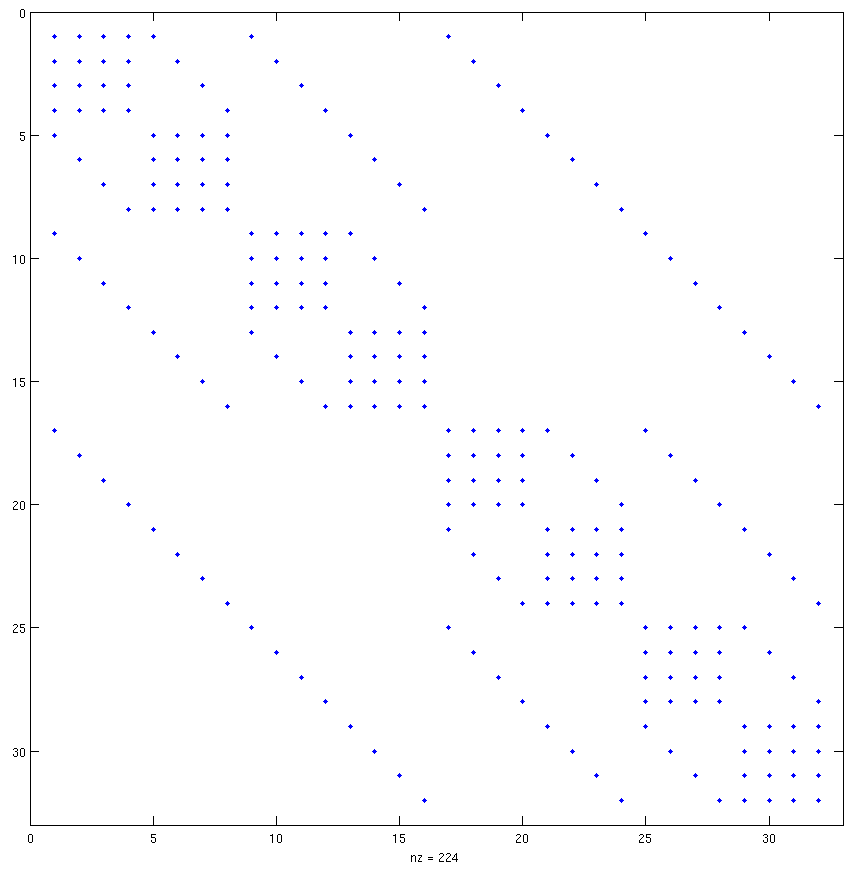
\includegraphics[width=4in]{chapters/spn_equations/group1.png}
  \end{center}
  \caption{\textbf{Sparsity pattern for 1-group $SP_7$
      discretization.} \textit{A $2\times 2 \times 2$ element mesh was
      used to show detail of the blocks formed by the discretization.}}
  \label{fig:group1}
\end{figure}
\begin{figure}[t!]
  \begin{center}
    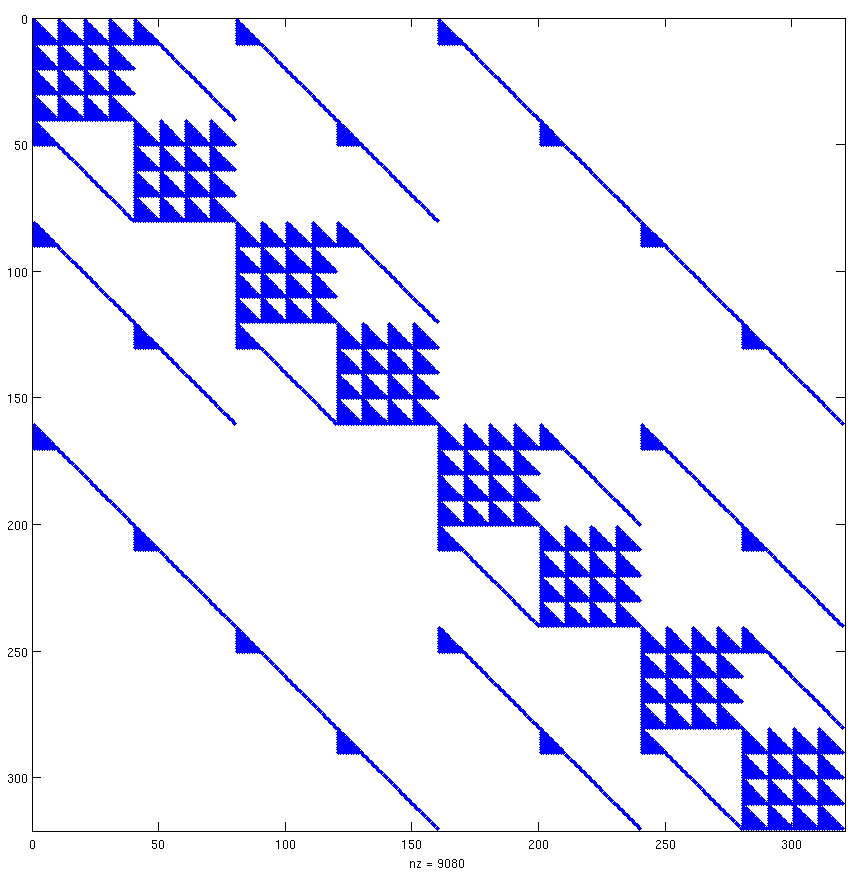
\includegraphics[width=4in]{chapters/spn_equations/group10ds.png}
  \end{center}
  \caption{\textbf{Sparsity pattern for 10-group $SP_7$ discretization
      with downscatter only.} \textit{A $2\times 2 \times 2$ element
      mesh was used to show detail of the blocks formed by the
      discretization.}}
  \label{fig:group10ds}
\end{figure}
\begin{figure}[t!]
  \begin{center}
    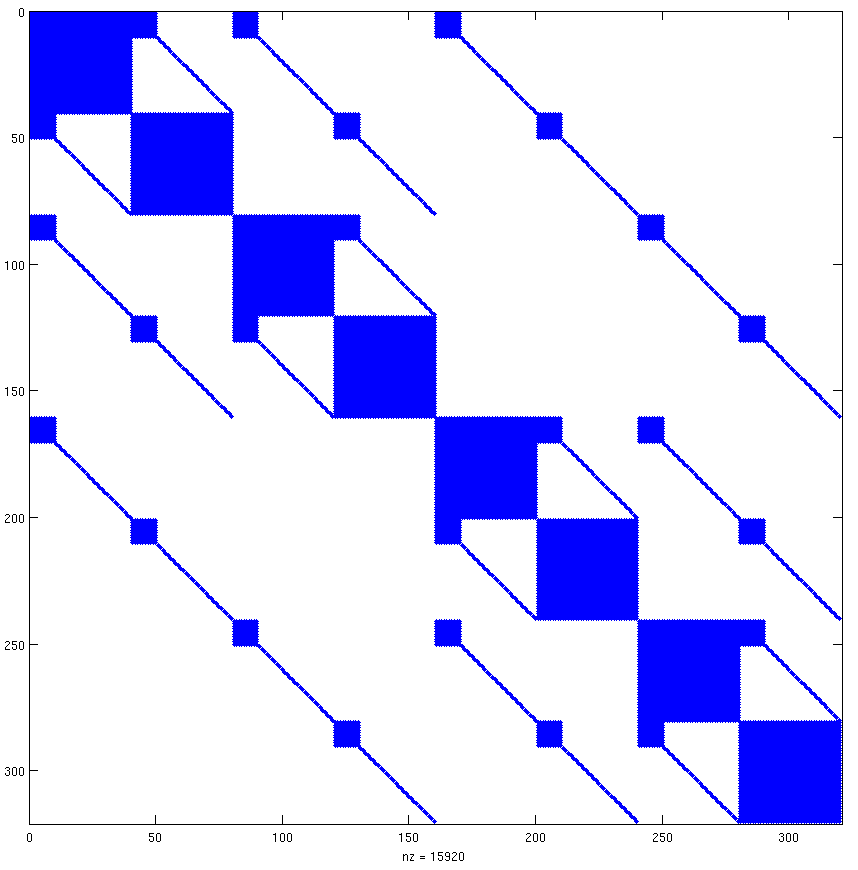
\includegraphics[width=4in]{chapters/spn_equations/group10us.png}
  \end{center}
  \caption{\textbf{Sparsity pattern for 10-group $SP_7$ discretization
      with downscatter and upscatter.} \textit{A $2\times 2 \times 2$ element
      mesh was used to show detail of the blocks formed by the
      discretization.}}
  \label{fig:group10us}
\end{figure}
We note a few key features of the sparsity plots. The first is that
for multigroup problems without full upscatter and downscatter
(i.e. Figure~\ref{fig:group10ds}), the resulting matrix is asymmetric
and therefore a linear solver that can handle asymmetric linear
systems is required. Nearly all problems of interest will not have
full upscattering or downscattering. Second we note the largely
diagonal character of these systems, although the blocks from
Eq~(\ref{eq:A_block_matrix}) are readily apparent. Our first attempt
at preconditioning this system will be to use the point Jacobi
preconditioning from \S\ref{subsubsec:basic_mcsa_preconditioning} due
to this diagonal form.

\clearpage

\subsection{Point Jacobi Spectral Analysis Results}
\label{subsec:spn_analysis_results}
Spectral radius computations were performed for the cases described
above for the point Jacobi preconditioned iteration matrix $\ve{H} =
\ve{I}-\ve{M}^{-1}\ve{A}$ with $\ve{M} =
diag(\ve{A})$. Table~\ref{tab:group1pj} gives the results for the
1-group case, Table~\ref{tab:group10dspj} for the 10-group case with
full downscatter only and Table~\ref{tab:group10uspj} for the 10-group
case with full downscatter and full upscatter.
\begin{table}[h!]
  \begin{center}
    \begin{tabular}{cccccc}\hline\hline
      \multicolumn{1}{c}{}& 
      \multicolumn{1}{c}{}& 
      \multicolumn{1}{c}{}& 
      \multicolumn{1}{c}{$SP_N$ Order}& 
      \multicolumn{1}{c}{}& 
      \multicolumn{1}{c}{} \\
       &   & \textbf{1} & \textbf{3} & \textbf{5} & \textbf{7}  \\
       & \textbf{0} & 0.0635 & 0.6722 & 1.3144 & 1.976 \\
       & \textbf{1} & 0.0666 & 0.6728 & 1.3141 & 1.9755 \\
      $P_N$ Order & \textbf{3} & 0.0666 & 0.6822 & 1.3141 & 1.9755 \\
       & \textbf{5} & 0.0666 & 0.6822 & 1.3278 & 1.9847 \\
       & \textbf{7} & 0.0666 & 0.6822 & 1.3278 & 1.9917 \\
      %%
      \hline\hline
    \end{tabular}
  \end{center}
  \caption{\textbf{Spectral radius results for the point Jacobi
      preconditioned iteration matrix with 1 energy group.}}
  \label{tab:group1pj}
\end{table}
\begin{table}[h!]
  \begin{center}
    \begin{tabular}{cccccc}\hline\hline
      \multicolumn{1}{c}{}& 
      \multicolumn{1}{c}{}& 
      \multicolumn{1}{c}{}& 
      \multicolumn{1}{c}{$SP_N$ Order}& 
      \multicolumn{1}{c}{}& 
      \multicolumn{1}{c}{} \\
       &   & \textbf{1} & \textbf{3} & \textbf{5} & \textbf{7}  \\
       & \textbf{0} & 0.0655 & 0.677 & 1.32 & 1.982 \\
       & \textbf{1} & 0.071 & 0.6777 & 1.319 & 1.982 \\
      $P_N$ Order & \textbf{3} & 0.071 & 0.687 & 1.327 & 1.9872 \\
       & \textbf{5} & 0.071 & 0.687 & 1.336 & 1.997 \\
       & \textbf{7} & 0.071 & 0.687 & 1.336 & 1.9995 \\
      %%
      \hline\hline
    \end{tabular}
  \end{center}
  \caption{\textbf{Spectral radius results for the point Jacobi
      preconditioned iteration matrix with 10 energy groups and full
      downscatter.}}
  \label{tab:group10dspj}
\end{table}
\begin{table}[h!]
  \begin{center}
    \begin{tabular}{cccccc}\hline\hline
      \multicolumn{1}{c}{}& 
      \multicolumn{1}{c}{}& 
      \multicolumn{1}{c}{}& 
      \multicolumn{1}{c}{$SP_N$ Order}& 
      \multicolumn{1}{c}{}& 
      \multicolumn{1}{c}{} \\
       &   & \textbf{1} & \textbf{3} & \textbf{5} & \textbf{7}  \\
       & \textbf{0} & 0.7283 & 0.81 & 1.47 & 2.1446 \\
       & \textbf{1} & 0.7317 & 0.8 & 1.46 & 2.1368 \\
      $P_N$ Order & \textbf{3} & 0.7317 & 0.91 & 1.526 & 2.2274 \\
       & \textbf{5} & 0.7317 & 0.91 & 1.5344 & 2.2562 \\
       & \textbf{7} & 0.7317 & 0.91 & 1.5345 & 2.2842 \\
      %%
      \hline\hline
    \end{tabular}
  \end{center}
  \caption{\textbf{Spectral radius results for the point Jacobi
      preconditioned iteration matrix with 10 energy groups, full
      downscatter and full upscatter.}}
  \label{tab:group10uspj}
\end{table}
It is readily apparent from the tabulated data that point Jacobi
preconditioning is insufficient. For problems of order $SP_5$ and
$SP_7$, the method will not converge at all and for the upscatter case
with $SP_3$ the spectral radius is still quite large for large $P_N$
orders and therefore convergence is expected to be slow. These
eigenvalues signal a need for a better preconditioning strategy to
both ensure and improve convergence for Monte Carlo methods.

\subsection{Block Jacobi Preconditioning}
\label{sec:spn_preconditioning}
If Monte Carlo methods are to be used to solve the $SP_N$ system of
equations, a different preconditioning strategy is required in order
to ensure convergence for systems of all $SP_N$ and $P_N$ orders with
arbitrary energy group structures. As another means of achieving this,
we look back to the sparsity plots we generated in
Figures~\ref{fig:group1}, \ref{fig:group10ds} and \ref{fig:group10us}
as well as the multigroup $SP_N$ equations. Initially, the diagonal
character of the system led us to try point Jacobi preconditioning
with only marginal results. From the sparsity plots we note the block
structure that ultimately arises from the multigroup scattering
matrices and their insertion into Eq~(\ref{eq:A_block_matrix}). When
full upscatter and downscatter are used the resulting blocks are
completely dense while only downscatter gives a lower triangular
scattering matrix and the block structure shown in
Figure~\ref{fig:group10ds}.

Based on this both block and diagonally dominant structure for
matrices formed by the general multigroup $SP_N$ equations, we instead
choose \textit{block Jacobi} preconditioning as a left preconditioner
for the system. Like point Jacobi preconditioning, block Jacobi
preconditioning extracts the diagonal elements of the matrix as the
preconditioner where now the elements extracted are the blocks on the
diagonal as shown on the left side of
Figure~\ref{fig:block_jacobi_ex}. Shown on the right side of
Figure~\ref{fig:block_jacobi_ex}, inversion of the preconditioner is
trivial with each diagonal block inverted separately. For the $SP_N$
equations, Eq~(\ref{eq:A_block_matrix}) gives a block size of
$N_g\times(N+1)/2$.
\begin{figure}[t!]
  \begin{center}
    \scalebox{1.5}{
    \input{chapters/spn_equations/block_jacobi.pdftex_t} }
  \end{center}
  \caption{\textbf{Block Jacobi preconditioning strategy used for the
      $SP_N$ equations.} \textit{Left: The preconditioner is formed by
      the diagonal blocks of the matrix. Right: Inversion of the
      preconditioner is trivial and decoupled by block.}}
  \label{fig:block_jacobi_ex}
\end{figure}
The inversion of this preconditioner is trivial as shown on the right
side of Figure~\ref{fig:block_jacobi_ex}. Each block can be inverted
individually and combined to form the inverse. In addition, in the
limit of a block size of one, the block Jacobi method reduces to the
point Jacobi method. For high performance implementations this has
several attractive properties. First, the blocks in the matrix come
from the energy/angle discretization of the transport equation as
given by Eq~(\ref{eq:A_block_matrix}). Each block on the diagonal is
bound to a mesh element in the system (note there are 8 blocks on the
diagonal in each of the sparsity patterns with a mesh of $2 \times 2
\times 2$) and therefore we expect the matrix elements forming the
block to be entirely local. Second, these blocks are typically dense
and nearly lower triangular for many transport problems meaning that
established dense matrix methods can be used for fast inversion.

\subsection{Block Jacobi Spectral Analysis Results}
\label{subsec:spn_analysis_results}
Spectral radius computations for the block Jacobi preconditioned
iteration matrix were performed for the same problems as the point
Jacobi preconditioned case. Table~\ref{tab:group1bj} gives the results
for the 1-group case, Table~\ref{tab:group10dsbj} for the 10-group
case with full downscatter only and Table~\ref{tab:group10usbj} for
the 10-group case with full downscatter and full upscatter. A block
size of $N_g\times(N+1)/2$ was used for the preconditioner in all
cases.
\begin{table}[h!]
  \begin{center}
    \begin{tabular}{cccccc}\hline\hline
      \multicolumn{1}{c}{}& 
      \multicolumn{1}{c}{}& 
      \multicolumn{1}{c}{}& 
      \multicolumn{1}{c}{$SP_N$ Order}& 
      \multicolumn{1}{c}{}& 
      \multicolumn{1}{c}{} \\
       &   & \textbf{1} & \textbf{3} & \textbf{5} & \textbf{7}  \\
       & \textbf{0} & 0.0635 & 0.1269 & 0.1444 & 0.1513 \\
       & \textbf{1} & 0.0666 & 0.1315 & 0.1474 & 0.1534 \\
      $P_N$ Order & \textbf{3} & 0.0666 & 0.1365 & 0.154 & 0.1592 \\
       & \textbf{5} & 0.0666 & 0.1365 & 0.1562 & 0.163 \\
       & \textbf{7} & 0.0666 & 0.1365 & 0.1562 & 0.164 \\
      %%
      \hline\hline
    \end{tabular}
  \end{center}
  \caption{\textbf{Spectral radius results for the block Jacobi
      preconditioned iteration matrix with 1 energy group.}}
  \label{tab:group1bj}
\end{table}
\begin{table}[h!]
  \begin{center}
    \begin{tabular}{cccccc}\hline\hline
      \multicolumn{1}{c}{}& 
      \multicolumn{1}{c}{}& 
      \multicolumn{1}{c}{}& 
      \multicolumn{1}{c}{$SP_N$ Order}& 
      \multicolumn{1}{c}{}& 
      \multicolumn{1}{c}{} \\
       &   & \textbf{1} & \textbf{3} & \textbf{5} & \textbf{7}  \\
       & \textbf{0} & 0.0647 & 0.1275 & 0.1449 & 0.1514 \\
       & \textbf{1} & 0.0686 & 0.1338 & 0.1484 & 0.1547 \\
      $P_N$ Order & \textbf{3} & 0.0687 & 0.1399 & 0.1582 & 0.1625 \\
       & \textbf{5} & 0.0692 & 0.1399 & 0.1582 & 0.1657 \\
       & \textbf{7} & 0.0678 & 0.1393 & 0.1624 & 0.166 \\
      %%
      \hline\hline
    \end{tabular}
  \end{center}
  \caption{\textbf{Spectral radius results for the block Jacobi
      preconditioned iteration matrix with 10 energy groups and full
      downscatter.}}
  \label{tab:group10dsbj}
\end{table}
\begin{table}[h!]
  \begin{center}
    \begin{tabular}{cccccc}\hline\hline
      \multicolumn{1}{c}{}& 
      \multicolumn{1}{c}{}& 
      \multicolumn{1}{c}{}& 
      \multicolumn{1}{c}{$SP_N$ Order}& 
      \multicolumn{1}{c}{}& 
      \multicolumn{1}{c}{} \\
       &   & \textbf{1} & \textbf{3} & \textbf{5} & \textbf{7}  \\
       & \textbf{0} & 0.1887 & 0.2267 & 0.2285 & 0.2286 \\
       & \textbf{1} & 0.4535 & 0.5044 & 0.5045 & 0.5045 \\
      $P_N$ Order & \textbf{3} & 0.4535 & 0.6453 & 0.6506 & 0.6506 \\
       & \textbf{5} & 0.4535 & 0.6453 & 0.6802 & 0.6818 \\
       & \textbf{7} & 0.4535 & 0.6453 & 0.6802 & 0.6927 \\
      %%
      \hline\hline
    \end{tabular}
  \end{center}
  \caption{\textbf{Spectral radius results for the block Jacobi
      preconditioned iteration matrix with 10 energy groups, full
      downscatter and full upscatter.}}
  \label{tab:group10usbj}
\end{table}

From the tabulated block Jacobi data it is clear that this is a viable
preconditioning choice for all $SP_N$ problems in term of Monte Carlo
solution methods. All cases were observed to have a spectral radius
below unity and often significantly smaller than that, greatly
improving convergence rates over the point Jacobi preconditioned
problem. Based on these results, the block Jacobi method should be the
first preconditioning strategy applied to more complicated problems
representative of physical systems.
\clearpage

%%---------------------------------------------------------------------------%%
\section{Fuel Assembly Criticality Calculations}
\label{sec:fuel_assembly_calcs}
Fuel assembly calculations are a critical piece of nuclear engineering
infrastructure for reactor core analysis and design. At this level,
individual fuel pins may be resolved at fine resolution in a variety
of configurations. As a sophisticated problem of interest to push the
limits of MCSA, a hot zero-power $17 \times 17$ pin assembly will be
used with varying energy group structure and $SP_N$ discretization in
a criticality calculation. A cross section along the vertical axis
showing homogenized fuel pin materials and the associated grid is
given by Figure~\ref{fig:problem3_radial_mat} while a cross section of
the materials configuration along the horizontal axis is given by
Figure~\ref{fig:problem3_axial_mat}. A detailed view of the assembly
bottom is given in Figure~\ref{fig:problem3_end}. On the top and
bottom of the assembly, vacuum conditions are used as well as on the
top and right boundaries in
Figure~\ref{fig:problem3_radial_mat}. Reflecting conditions are used
on the left and bottom boundaries of
Figure~\ref{fig:problem3_radial_mat}, effectively giving a
representation of one quarter of the assembly. For the spatial
discretization, each fuel pin (gray regions in
Figure~\ref{fig:problem3_radial_mat}) is resolved by a $2 \times 2$
mesh with materials and cross sections homgenized over this region.
\begin{figure}[t!]
  \begin{center}
    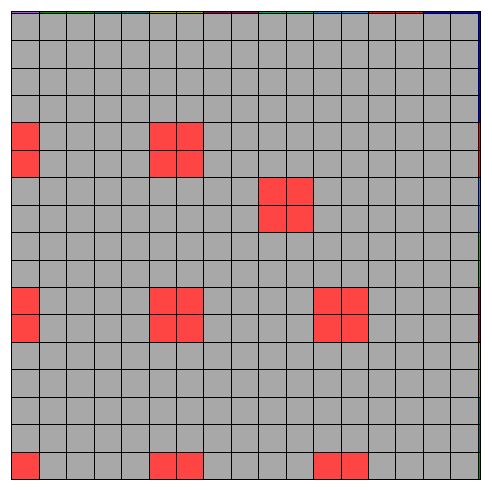
\includegraphics[width=4in]{chapters/spn_equations/problem3_radial_mat.png}
  \end{center}
  \caption{\textbf{Fuel assembly mesh and geometry cross section.}
    \textit{Reflecting boundaries are used on the left and lower
      boundaries to create a complete $17 \times 17$ assembly
      geometry. Gray regions are homogenized fuel and red regions are
      homogenized moderator. Each fuel pin is resolved by a $2 \times
      2$ mesh.}}
  \label{fig:problem3_radial_mat}
\end{figure}
\begin{figure}[t!]
  \begin{center}
    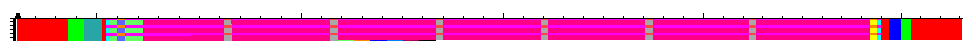
\includegraphics[width=6.0in]{chapters/spn_equations/problem3_axial_mat.png}
  \end{center}
  \caption{\textbf{Fuel assembly geometry cross section.} \textit{The
      geometry is subdivided along the axial direction into 50 zones
      spaced to capture material boundaries. Important details include
      spacer grids along the length of the fuel pins and reactor core
      structures on the top and bottom of the assembly. Lighter purple
      material in the center of the assembly is moderator and darker
      purple/red material is fuel.}}
  \label{fig:problem3_axial_mat}
\end{figure}
\begin{figure}[t!]
  \begin{center}
    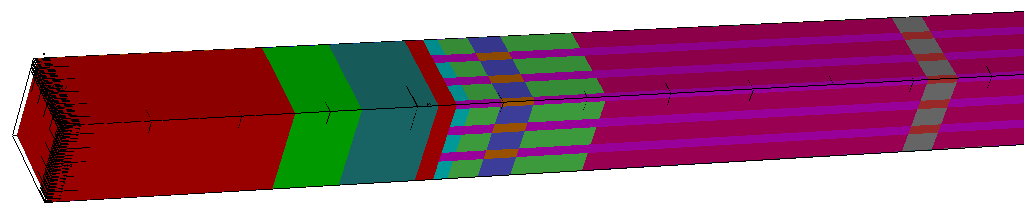
\includegraphics[width=6.0in]{chapters/spn_equations/problem3_end.png}
  \end{center}
  \caption{\textbf{Fuel assembly geometry end detail.}
    \textit{Reactor core structure including spacer grids and plenum
      has been included. Lighter purple material on the right of the
      figure is moderator and darker purple/red material is fuel.}}
  \label{fig:problem3_end}
\end{figure}

Significant geometric details are contained in the model including
spacer grids, fuel pins with homogenized cladding and gas gap, core
plenum, and moderator with boron. Group cross sections and other
discrete nuclear data are generated as needed by a cross-section
processing module dependent on the meshing parameters used to
discretize the geometry and single-dimension pin-cell calculations for
initial flux spectrum generation. Table~\ref{tab:problem3_parameters}
gives the primary design parameters for the fuel assembly
calculations.
\begin{table}[h!]
  \begin{center}
    \begin{tabular}{ll}\hline\hline
      \multicolumn{1}{l}{\textbf{Parameter}} & 
      \multicolumn{1}{l}{\textbf{Value}} \\
      Power Level & 0 MW \\
      Inlet Temperature & 326.85C \\
      Fuel Temperature & 600C \\
      Boron Concentration & 1300 ppm \\
      Moderator Density & 0.743 g/cc \\
      Helium Density & \sn{1.79}{-4} g/cc \\
      Zirconium Density & 6.56 g/cc \\
      Stainless Steel Density & 8.0 g/cc \\
      Inconel Density & 8.19 g/cc \\
      UO2 Density & 10.257 g/cc \\
      Fuel Pin Radius (w/o clad) & 0.4096 cm \\
      %%
      \hline\hline
    \end{tabular}
  \end{center}
  \caption{\textbf{Design parameters for the $17 \times 17$ pin fuel
      assembly criticality calculation.}}
  \label{tab:problem3_parameters}
\end{table}

To generate the multiplication factor and steady-state flux
distribution for this problem, at every eigenvalue iteration MCSA is
used to solve the resulting $SP_N$ problem using the provided fission
source. Algorithm~\ref{alg:power_iteration} presents the use of MCSA
within a power iteration strategy to find the multiplication factor.
\begin{algorithm}[h!]
  \caption{Power Iteration MCSA Scheme}
  \label{alg:power_iteration}
  \begin{algorithmic}
    \State $k_0 =$ initial guess
    \State $\mathbf{\Phi}_0 =$ initial guess
    \State $n = 0$
    \While{$|\frac{k^n - k^{n-1}}{k^n}| < \epsilon$}
    \Comment{Iterate until convergence of the eigenvalue}
    \State $\mathbf{M} \mathbf{\Phi}^{n+1} = \frac{1}{k^n} \mathbf{F} \mathbf{\Phi}^n$
    \Comment{Solve for the new flux state with MCSA}
    \State $k^{n+1} = k^n \frac{\int \mathbf{F} \mathbf{\Phi}^{n+1} d\mathbf{r}}{\int
      \mathbf{F} \mathbf{\Phi}^n d\mathbf{r}}$
    \Comment{Update the multiplication factor}
    \State $n = n+1$
    \EndWhile
  \end{algorithmic}
\end{algorithm}
Here, $\mathbf{M}$ is the transport operator generated on the
left-hand side of the $SP_N$ discretization, $\mathbf{F}$ is the
fission matrix, and $\mathbf{\Phi}$ the multigroup neutron flux. This
problem is significantly more complicated than the simple test problem
used for the previous spectral analysis. Fission has been introduced
into the set of equations and the addition of moderator into the
system will increase the amount of scattering, creating a
significantly more difficult problem manifesting itself in an
iteration matrix with a larger spectral radius. When using MCSA, the
linear operator applied to $\mathbf{\Phi}^{n+1}$ at each eigenvalue
iteration will dictate convergence and remain unchanged throughout the
computation\footnote{The operator will change if, for example, physics
  feedback through temperature or potentially burnup is
  considered. These additional physics will modify the cross sections
  used to assemble $\mathbf{M}$. The calculations presented here will
  consist of a single eigenvalue calculation with a static
  $\mathbf{M}$.} while the addition of fission to the system will only
modify the source of neutrons and the multiplication factor while not
affecting Monte Carlo transport.
 
\clearpage 

\subsection{Preliminary Jacobi Preconditioned Calculations}
\label{subsec:jacobi_prec_assembly_calc}
Based on the success of block Jacobi preconditioning with the test
problem used for the spectral radius parameter study, we use it first
to solve the $17 \times 17$ fuel assembly problem. A single energy
group problem was first solved with $SP_1$ discretization, effectively
giving the one-speed neutron diffusion system for the fuel assembly
resulting in 20,088 degrees of freedom in the
problem. Figure~\ref{fig:block_jacobi_res_mcsa} gives the residual
infinity norm as a function of iteration for the MCSA linear solve in
the first eigenvalue iteration using 25,000 stochastic histories at
every iteration for the adjoint Neumann-Ulam solve.
\begin{figure}[t!]
  \begin{center}
    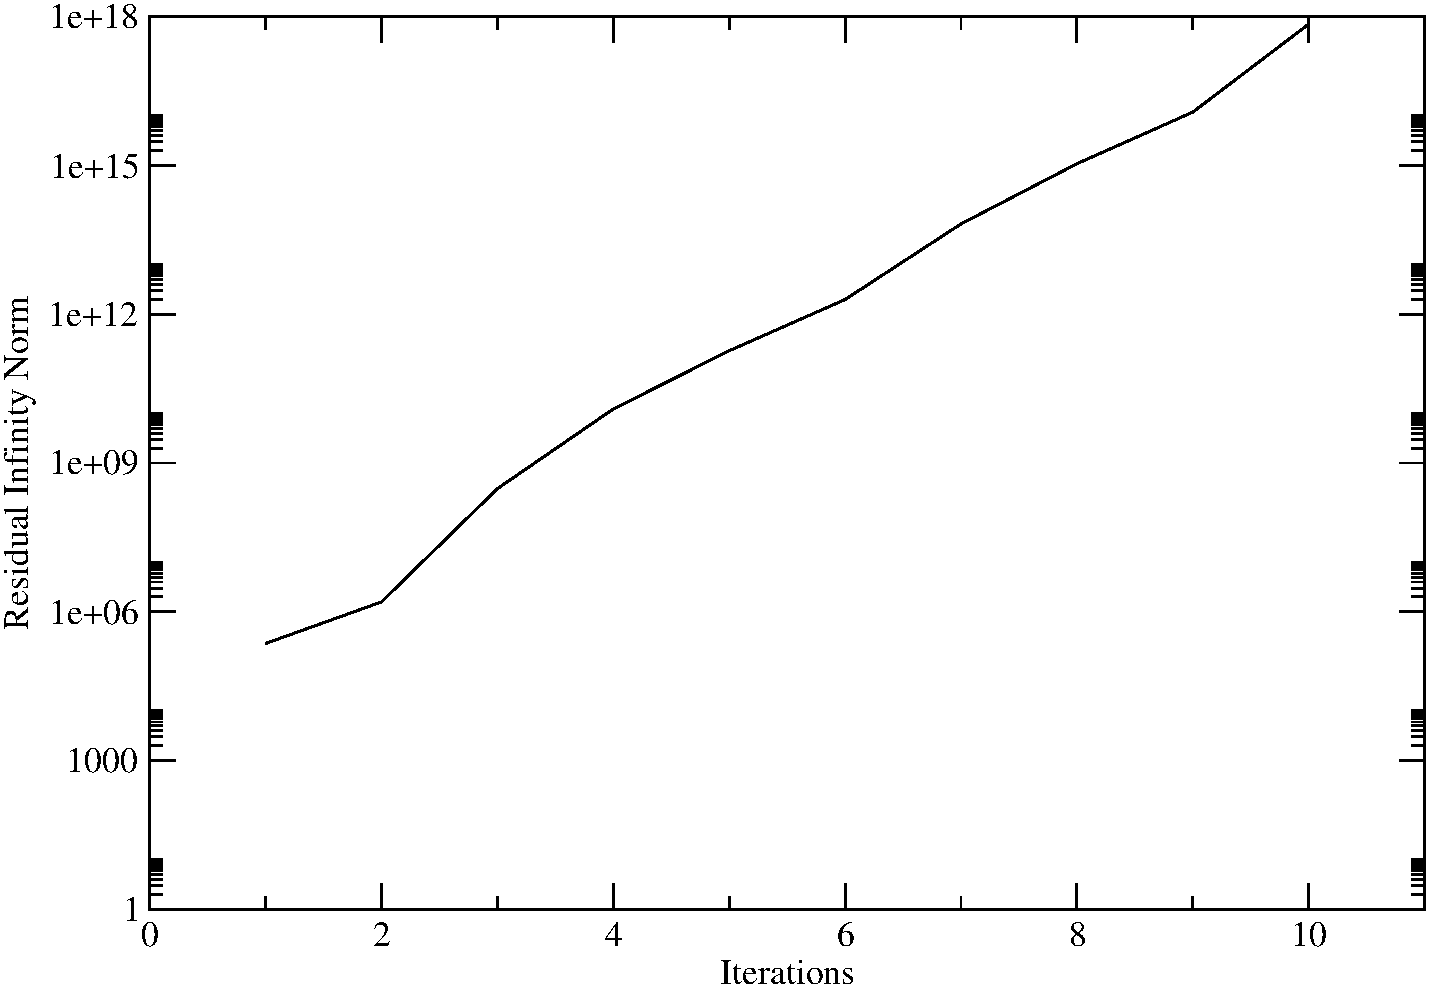
\includegraphics[width=6in]{chapters/spn_equations/block_jacobi_res.pdf}
  \end{center}
  \caption{\textbf{Residual infinity norm vs. iteration for the block
      Jacobi preconditioned MCSA solve during the first eigenvalue
      iteration of the 1-group $17 \times 17$ fuel assembly problem.}
    \textit{Convergence was not achieved with the block Jacobi
      preconditioned method.}}
  \label{fig:block_jacobi_res_mcsa}
\end{figure}
Convergence was not achieved as noted by the rapid rise in the
residual over a few iterations. Based on the spectral radius
computations performed, these results are not in line with
expectations for this problem. Additional computations performed with
\sn{1}{6} histories per iteration exhibited the same divergent
behavior at a significant computational cost and compute time. Even if
the problem may be ill-conditioned, we do expect convergence of
MCSA. To investigate further, a block Jacobi preconditioned Richardson
iteration was used to solve the same
problem. Figure~\ref{fig:block_jacobi_res_richardson} gives the
residual infinity norm as a function of iteration for the Richardson
linear solve in the first eigenvalue iteration.
\begin{figure}[t!]
  \begin{center}
    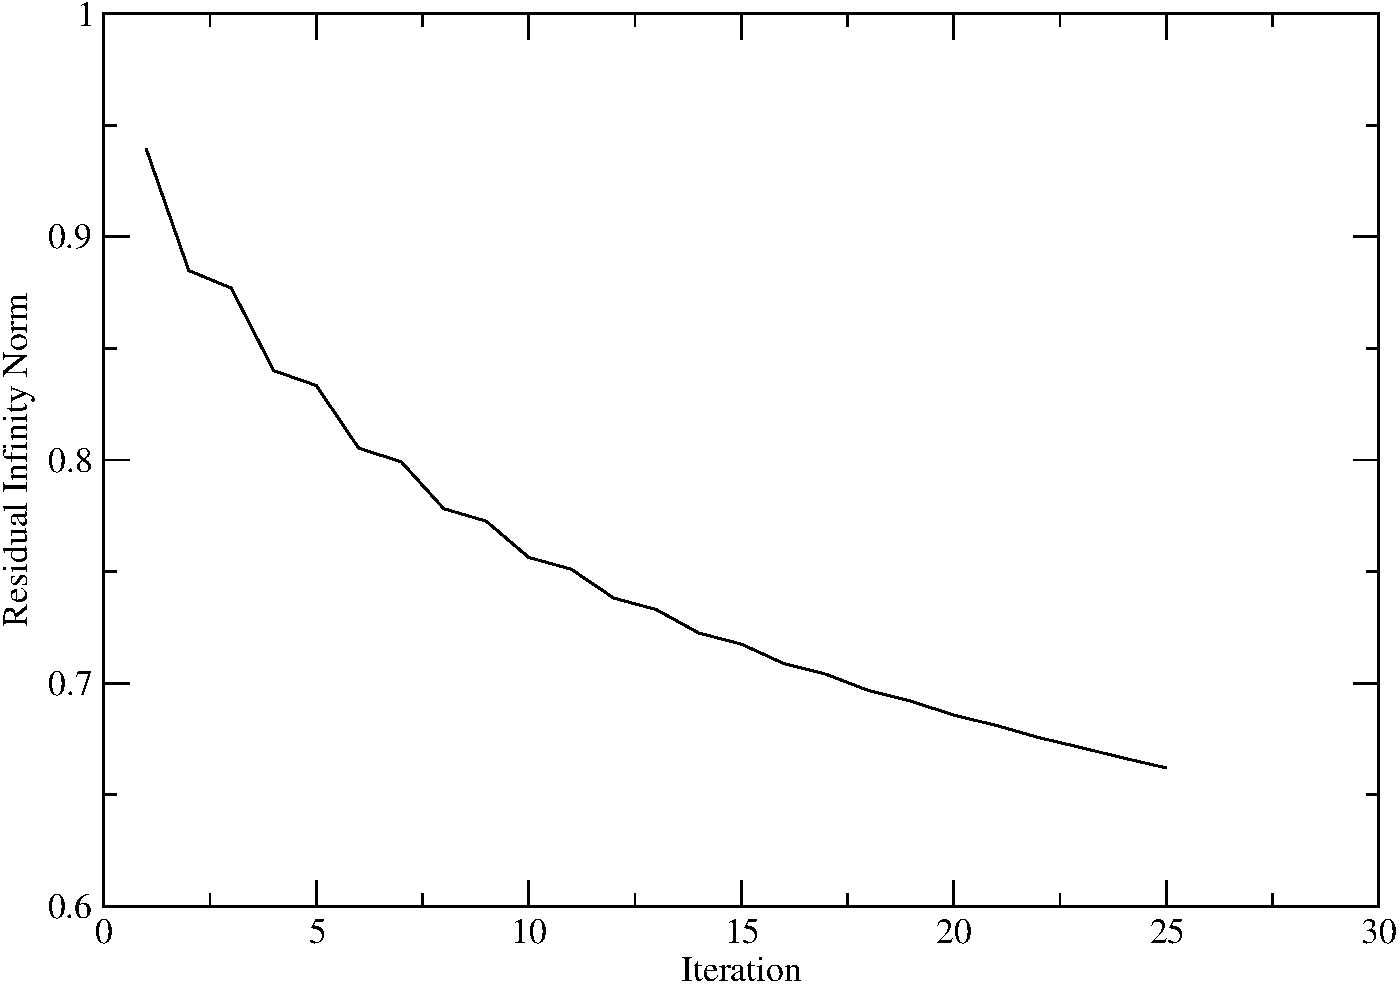
\includegraphics[width=6in]{chapters/spn_equations/block_jacobi_rich_res.pdf}
  \end{center}
  \caption{\textbf{Residual infinity norm vs. iteration for the block
      Jacobi preconditioned Richardson solve during the first
      eigenvalue iteration of the 1-group $17 \times 17$ fuel assembly
      problem.} \textit{A spectral radius near 1 was observed for the
      iteration matrix.}}
  \label{fig:block_jacobi_res_richardson}
\end{figure}
Poor converge is observed for the Richardson iteration, however,
convergence is achieved meaning that the preliminary criteria needed
to satisfy MCSA convergence has also been met. The number of
iterations required for the Richardson iteration to converge will give
an approximation for the spectral radius via
Eq~(\ref{eq:linear_k_iter_norm3}). With 7291 iterations required to
converge to a tolerance of $\sn{1}{-6}$, $\rho(\mathbf{H}) \approx
0.998$, nearing the limits of MCSA applicability and well beyond the
spectral radii generated in the initial spectral analysis.

Based on these results, it then appears that even if the simple
criteria of a spectral radius of less than one is met and the
Richardson iteration will converge with the same preconditioning, MCSA
still may not converge. We then expect the issue to reside with the
Neumann-Ulam solve providing the correction as the Richardson
iteration is known to provide the correct result. Furthermore, the
fact that the spectral radius is less than one means that the
stochastic histories in the block Jacobi preconditioned Neumann-Ulam
method are eventually being terminated by the weight cutoff as no
artificial absorption was used for these preliminary
calculations. Based on this, the correction being generated by the
Neumann-Ulam solve is the component of MCSA causing a divergent
solution.

\subsection{MCSA Breakdown}
\label{subsec:mcsa_break_down}
For the fuel assembly problem, the initial block Jacobi
preconditioned\footnote{For 1-group $SP_1$ problems the block size is
  1, giving a point Jacobi preconditioner.}  calculations used a
one-speed $SP_1$ discretization, effectively giving a diffusion
system. To study the breakdown of MCSA at iteration matrix spectral
radii near one, we will use a simpler homogeneous 2-dimensional
one-speed neutron diffusion system to isolate this behavior. In this
system, we can vary the cross sections while maintaining a fixed grid
in order to achieve varying spectral radii. For these studies, we
neglect fission as MCSA behavior is dictated by the transport operator
$\mathbf{M}$ in an eigenvalue scheme with the fission matrix used to
generate a fixed source.

\subsubsection{Model Diffusion Problem}
\label{subsec:model_problem}
For our breakdown study, we choose the one-speed, two-dimensional
neutron diffusion equation as a model problem
\citep{duderstadt_nuclear_1976}:
\begin{equation}
  -\boldsymbol{\nabla} \cdot D \boldsymbol{\nabla} \phi + \Sigma_a
  \phi = S\:,
  \label{eq:diffusion_eq}
\end{equation}
where $\phi$ is the neutron flux, $\Sigma_a$ is the absorption cross
section, and $S$ is the source of neutrons. In addition, $D$ is the
diffusion coefficient defined as:
\begin{equation}
  D = \frac{1}{3 ( \Sigma_t - \bar{\mu}\Sigma_s )}\:,
  \label{eq:diffusion_coeff}
\end{equation}
where $\Sigma_s$ is the scattering cross section, $\Sigma_t = \Sigma_a
+ \Sigma_s$ is the total cross section, and $\bar{\mu}$ is the cosine
of the average scattering angle. For simplicity, we will take
$\bar{\mu} = 0$ for our analysis giving $D=(3 \Sigma_t)^{-1}$. In
addition, to further simplify we will assume a homogeneous domain such
that the cross sections remain constant throughout. Doing this permits
us to rewrite Eq~(\ref{eq:diffusion_eq}) as:
\begin{equation}
  -D \boldsymbol{\nabla}^2 \phi + \Sigma_a \phi = S\:.
  \label{eq:diffusion_eq_simple}
\end{equation}

We choose a finite difference scheme on a square Cartesian grid to
discretize the problem. For the Laplacian, we choose the 9-point
stencil shown in Figure~\ref{fig:stencil} over a grid of size $h$
\citep{leveque_finite_2007}:
\begin{multline}
  \nabla^2_9\phi = \frac{1}{6h^2}[4 \phi_{i-1,j} + 4 \phi_{i+1,j}
    + 4 \phi_{i,j-1} + 4 \phi_{i,j+1} + \phi_{i-1,j-1}\\ +
    \phi_{i-1,j+1} + \phi_{i+1,j-1} + \phi_{i+1,j+1} - 20
    \phi_{i,j}]\:.
  \label{eq:nine_point_stencil}
\end{multline}
\begin{figure}[t!]
  \begin{center}
    \scalebox{1.25}{\input{chapters/spn_equations/stencil.pdftex_t}}
  \end{center}
  \caption{\textbf{Nine-point Laplacian stencil.}}
  \label{fig:stencil}
\end{figure}
We then have the following linear system to solve:
\begin{multline}
  -\frac{1}{6h^2}[4 \phi_{i-1,j} + 4 \phi_{i+1,j} + 4
    \phi_{i,j-1} + 4 \phi_{i,j+1} + \phi_{i-1,j-1}\\ + \phi_{i-1,j+1}
    + \phi_{i+1,j-1} + \phi_{i+1,j+1} - 20 \phi_{i,j}] + \Sigma_a
  \phi_{i,j} = s_{i,j}\:,
  \label{eq:fd_system}
\end{multline}
and in operator form:
\begin{equation}
  \ve{D}\boldsymbol{\phi}=\ve{s}\:,
  \label{eq:operator_system}
\end{equation}
where $\ve{D}$ is the diffusion operator, $\ve{s}$ is the source in
vector form and $\boldsymbol{\phi}$ is the vector of unknown fluxes.

To close the system, a set of boundary conditions is required. In the
case of a non-reentrant current condition applied to all global
boundaries of the domain, we choose the formulation of Duderstadt by
assuming the flux is zero at some ghost point beyond the
grid. Consider for example the equations on the $i=0$ boundary of the
domain:
\begin{multline}
  -\frac{1}{6h^2}[4 \phi_{-1,j} + 4 \phi_{1,j} + 4 \phi_{0,j-1} +
    4 \phi_{0,j+1} + \phi_{-1,j-1}\\ + \phi_{-1,j+1} + \phi_{1,j-1} +
    \phi_{1,j+1} - 20 \phi_{0,j}] + \Sigma_a \phi_{0,j} = s_{0,j}\:.
  \label{eq:x_min_bnd}
\end{multline}
Here we note some terms where $i=-1$ and therefore are representative
of grid points beyond the boundary of the domain. We set the flux at
these points to be zero, giving a valid set of equations for the $i=0$
boundary:
\begin{multline}
  -\frac{1}{6h^2}[4 \phi_{1,j} + 4 \phi_{0,j-1} + 4 \phi_{0,j+1}
    \\ + \phi_{-1,j+1} + \phi_{1,j-1} + \phi_{1,j+1} - 20 \phi_{0,j}]
  + \Sigma_a \phi_{0,j} = s_{0,j}\:.
  \label{eq:x_min_bnd_2}
\end{multline}
We repeat this procedure for the other boundaries of the domain. For
reflecting boundary conditions, the net current across a boundary is
zero.

\subsubsection{MCSA Breakdown Analysis}
\label{subsubsec:breakdown_analysis}
For each solver and estimator combination, the spectral radius of the
iteration matrix generated by the diffusion problem was varied by
changing the absorption cross section from 0.25 to 100 while fixing
the grid size at $100 \times 100$ with $h = 0.1$ and a fixed
scattering cross section of unity. For each parameter variation, a
minimum of one stochastic history per degree of freedom (DOF) in the
problem was used to compute the Monte Carlo correction. If the solver
could not converge in less than 100 iterations, the number of
histories was increased by increments of 5,000 until convergence was
achieved in less than 100 iterations. The number of iterations
required to converge MCSA and the time to converge was recorded as a
means to capture the breakdown.

Figure~\ref{fig:breakdown_iterations} gives the number of iterations
required to converge for the chosen number of histories per iteration
given by Figure~\ref{fig:breakdown_histories} using the adjoint solver
with the collision and expected value estimators and the forward
solver with the collision estimator. For spectral radii less than
0.97, all MCSA problems converged with 1 history per DOF (10,000 for
this problem) with the number of iterations required to converge
increasing as a function of spectral radius. Near a spectral radius of
0.97, the number of histories required to converge MCSA in less than
100 iterations takes a dramatic rise that exhibits neither exponential
nor power law behavior. As the spectral radius approaches 1, the
number of histories required becomes significant and effectively
impractical to compute. Even with this simple diffusion problem, the
behavior is consistent with that observed for the fuel assembly
problem with $SP_1$ discretization. In that case, we estimated a
spectral radius of $\approx 0.998$, larger than any of the spectral
radii that could be computed within even 90 minutes of compute time
for this simple two dimensional problem. For that problem, even
1,000,000 histories ($\approx 50$ per DOF) was not enough to provide
convergence. Even if single solve times of an hour can be tolerated,
dozens of solves are typically required to compute the multiplication
factor and flux spectrum within the $SP_N$ eigenvalue scheme for more
difficult problems like the fuel assembly, making the method unusable.
\begin{figure}[t!]
  \begin{center}
    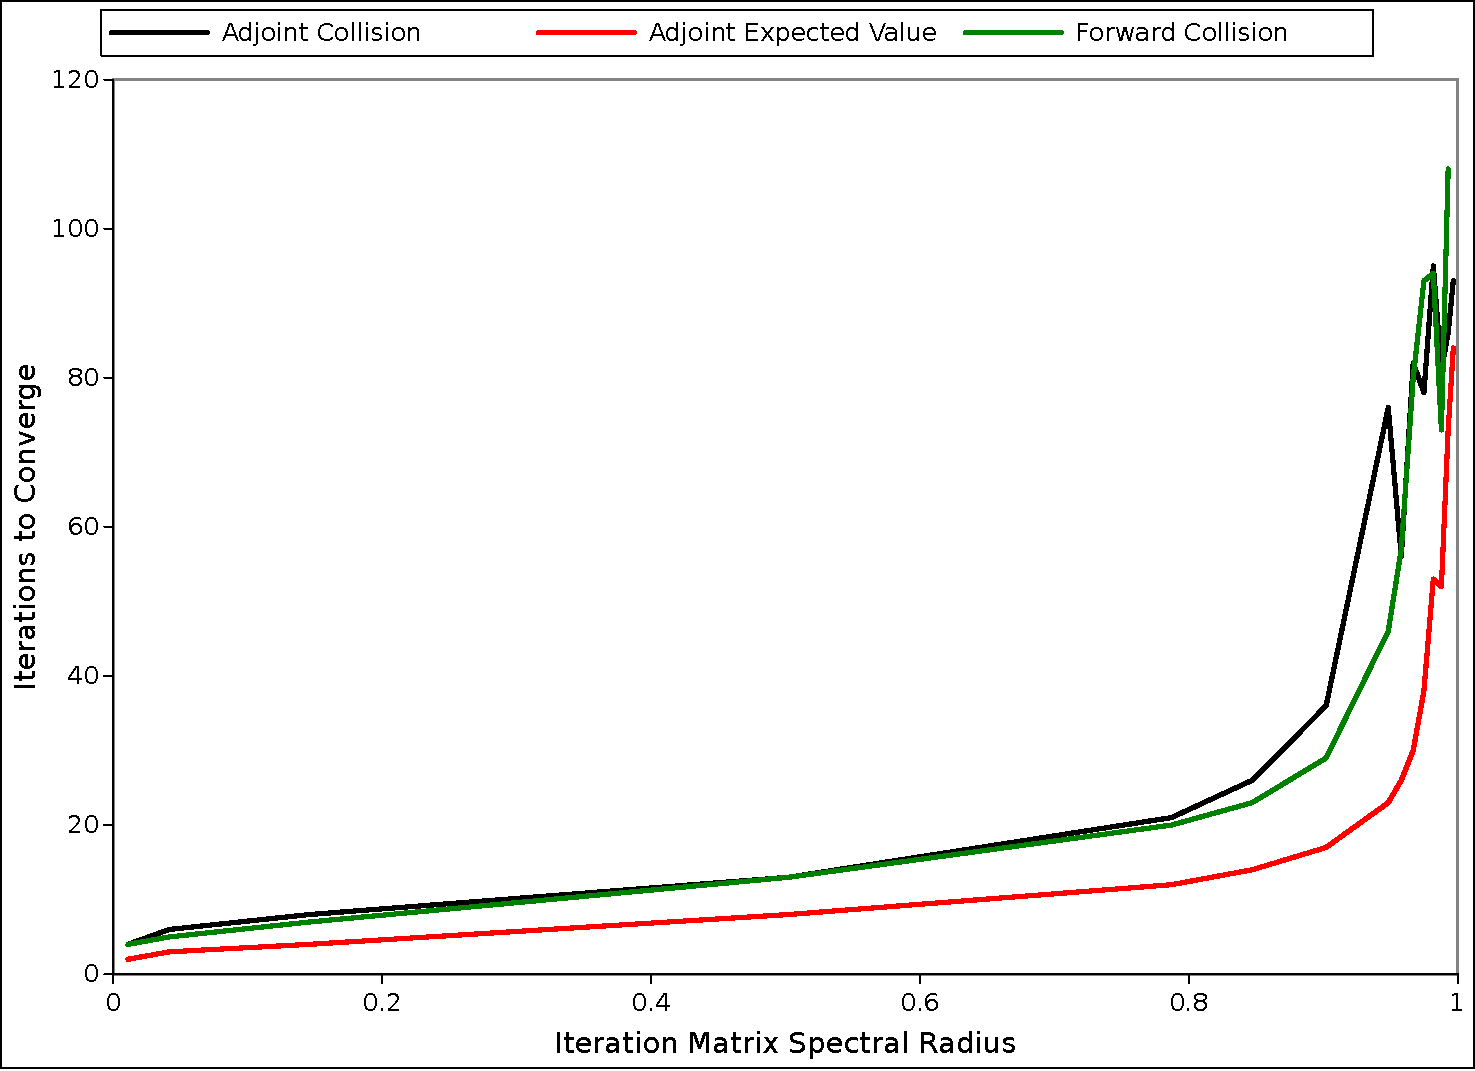
\includegraphics[width=6in]{chapters/spn_equations/breakdown_iterations.pdf}
  \end{center}
  \caption{\textbf{Iterations required to converge as a function of
      spectral radius for the neutron diffusion problem.} \textit{The
      number of histories was increased to achieve convergence in less
      than 100 iterations. At least 10,000 histories were used for
      each calculation.}}
  \label{fig:breakdown_iterations}
\end{figure}
\begin{figure}[t!]
  \begin{center}
    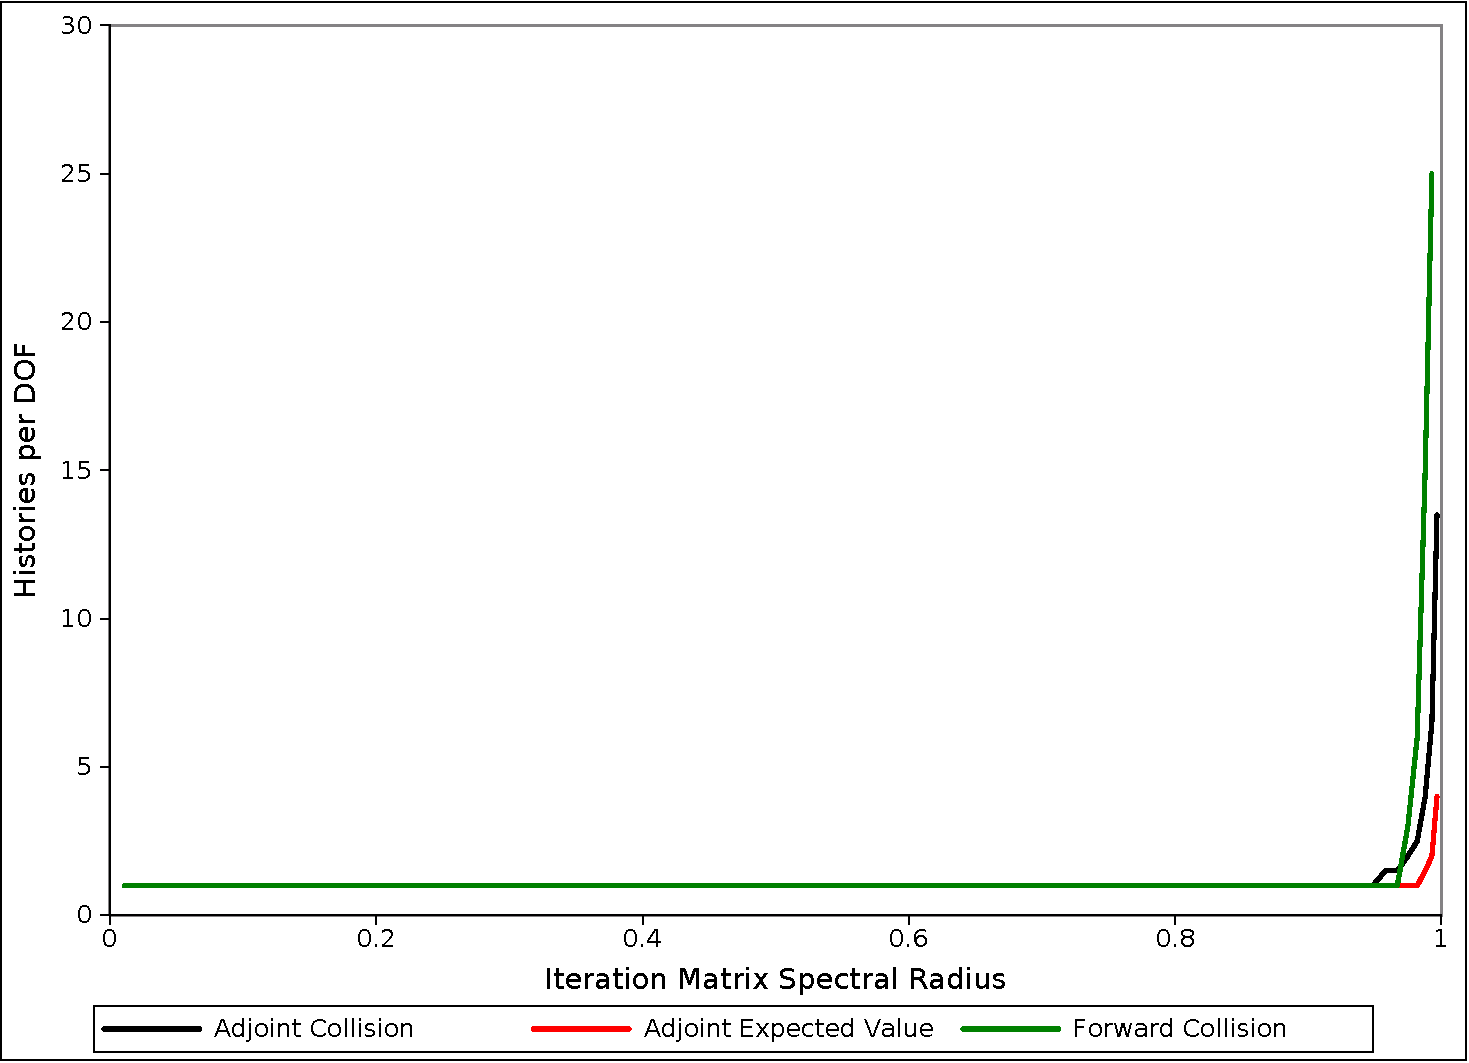
\includegraphics[width=6in]{chapters/spn_equations/breakdown_histories.pdf}
  \end{center}
  \caption{\textbf{Histories per DOF required to converge as a
      function of spectral radius for the neutron diffusion problem.}
    \textit{The number of histories was increased to achieve
      convergence in less than 100 iterations. At least 10,000
      histories were used for each calculation with 10,000 DOFs in the
      problem.}}
  \label{fig:breakdown_histories}
\end{figure}

In addition to the significantly larger number of histories required
for to achieve convergence for ill-conditioned problems another
penalty is paid due to histories that take longer to
compute. Figure~\ref{fig:breakdown_time} gives the CPU time in seconds
required to compute a single random walk averaged over the entire set
of histories run in the calculation over all iterations. As the
spectral radius increases (correlating to a higher ratio of scattering
in the system) the random walk lengths increase, using more CPU time
to finish the computation. Compared to spectral radii of 0.5, larger
spectral radii over 0.97 have histories that require two orders of
magnitude more computation time. This significant increase in
computation time per history coupled with the significant increase in
the number of histories required to converge is evidence that for
problems with spectral radii above $\approx 0.97$, using MCSA to solve
any problems of interest is entirely ineffective and not practical. We
therefore require a more expansive set of preconditioning techniques
to move the eigenvalue spectrum of the $SP_N$ problem into a regime in
which MCSA is more applicable and in which performance is improved.
\begin{figure}[t!]
  \begin{center}
    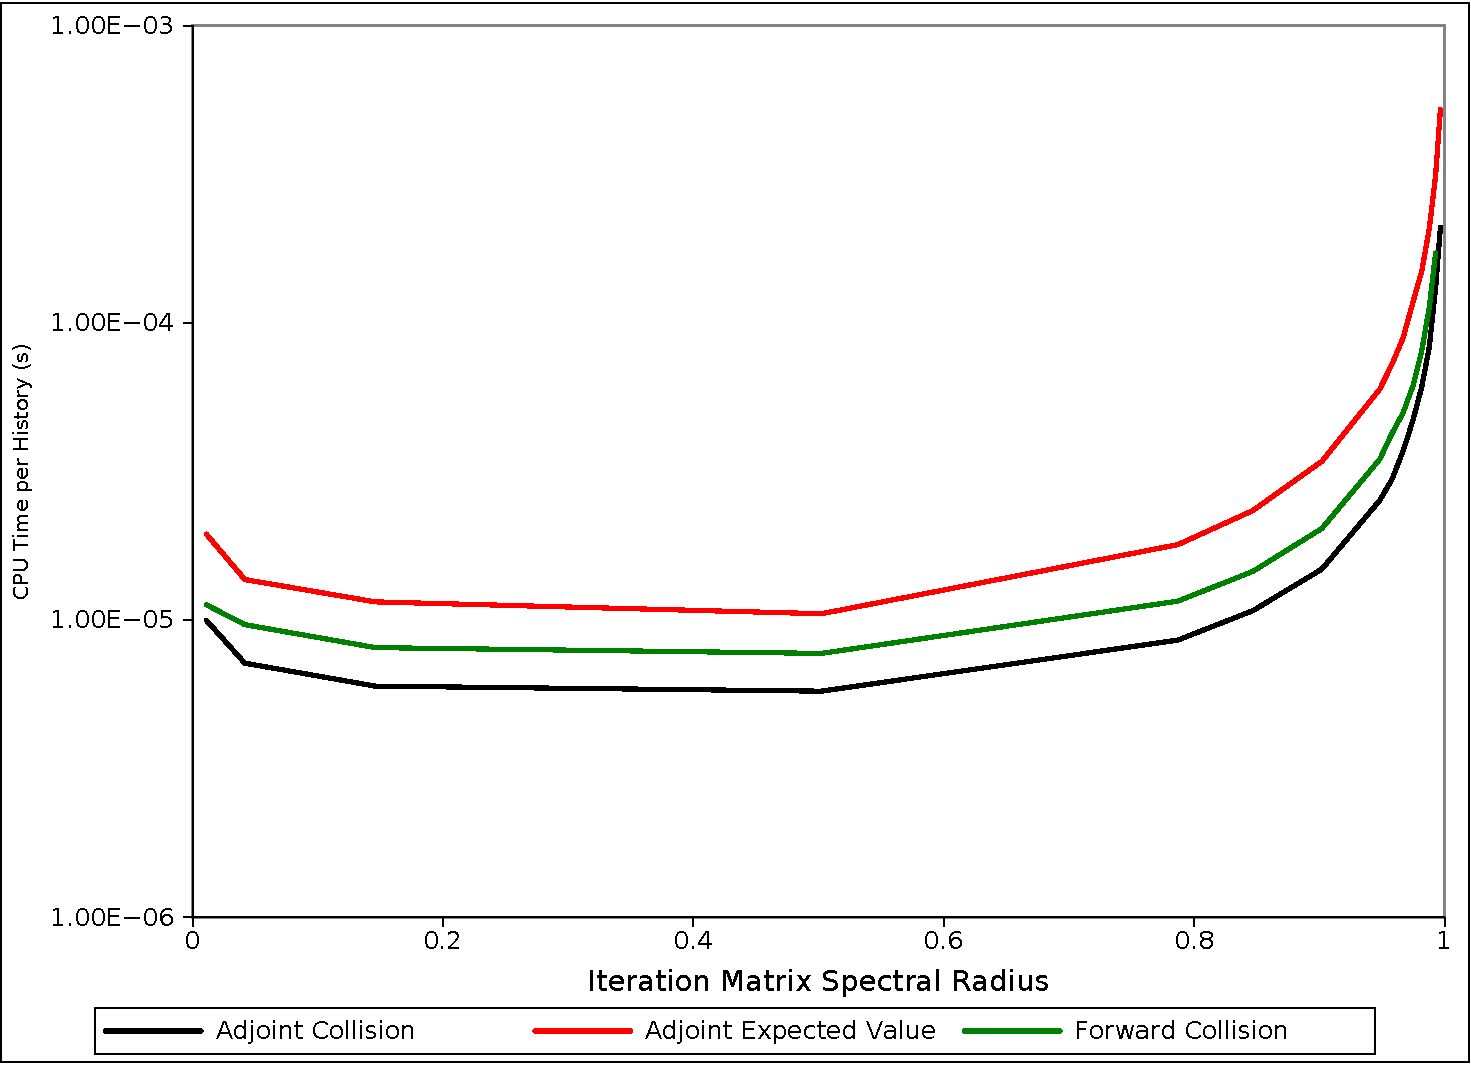
\includegraphics[width=6in]{chapters/spn_equations/breakdown_time.pdf}
  \end{center}
  \caption{\textbf{CPU time per history as a function of spectral
      radius for the neutron diffusion problem.} \textit{As the
      spectral radius grows, so do the length of the random
      walks. Longer random walks require more CPU time to compute.}}
  \label{fig:breakdown_time}
\end{figure}

\clearpage

%%---------------------------------------------------------------------------%%
\section{Advanced Preconditioning Strategies}
\label{subsec:spn_advanced_preconditioning}
For the fuel assembly criticality problem presented in the previous
section, the spectral radius was near one using Jacobi preconditioning
and in a regime in which MCSA breakdown is observed. In this regime
the number of stochastic histories required to converge MCSA increases
rapidly and the resulting poor performance is compounded by those
histories being increasingly expensive to compute. To overcome this
difficulty, advanced preconditioning strategies for the $SP_N$ problem
are required beyond simple Jacobi methods that can reduce the spectral
radius into a region of better MCSA performance. Several modern
algebraic preconditioning strategies will be presented here and used
within the explicit preconditioning framework given by
Eq~(\ref{eq:left_right_mcsa}). Data showing their effects on MCSA
solutions of the fuel assembly criticality problem will be presented.

\subsection{ILUT Preconditioning}
\label{subsec:spn_ilut_preconditioning}
Incomplete lower-upper (ILU) factorizations of the linear operator can
be used a simple mechanism to form an approximate inverse of a
preconditioner. To build the factorization, the sparse upper and lower
triangular factors, $\mathbf{L}$ and $\mathbf{U}$, are computed such
that the residual matrix formed by the factorization
\citep{saad_iterative_2003}:
\begin{equation}
  \mathbf{R} = \mathbf{L} \mathbf{U} - \mathbf{A} \:,
  \label{eq:ilu_residual_matrix}
\end{equation}
has a specified sparsity pattern and element magnitude. When a
magnitude threshold is used, elements generated in the factors below
that magnitude are dropped, resulting in ILU threshold (ILUT)
preconditioning. The sparsity pattern in this case is determined from
the input matrix to be preconditioned and the number of elements
maintained in the factor is specified by a fill level parameter. A
fill level of 1 will generate the same number of elements as the
sparsity pattern of the input matrix while a fill level of 2 will
contain twice as many elements in the factorization, resulting in a
better representation of the true LU factorization. The inverse of the
lower and upper triangular factors may then be easily inverted by
means of simple elimination to produce the preconditioner. For MCSA,
$\mathbf{L}^{-1}$ will be used on the left and $\mathbf{U}^{-1}$ on
the right to precondition the system.

For modern subspace methods, only the action to the preconditioner on
a vector is required for efficient implementations and therefore a
triangular solve can be used for this purpose. For the explicit
preconditioning scheme presented in Eq~(\ref{eq:left_right_mcsa}), the
fully inverted operator must be generated in order to build the set of
probabilities and weights required for Monte Carlo
sampling. Therefore, for a linear system of size $N$, $N$ triangular
solves will be required in order to extract the inverse matrices from
production ILU implementations. In addition, parallel implementations
typically generate lower and upper factors that are only triangular
locally, providing an easily parallelizable mechanism to generate the
action of the preconditioner inverse. A consequence of this choice for
parallel scalability is a degradation of the preconditioning quality
as the size of the parallel system is increased. For serial
computations, the triangular factorization is potentially exact
depending on the parameters chosen while at thousands of parallel
tasks, the global triangular factors differ significantly from the true
factorization. As a result, more iterations are required at higher
levels of parallelism to converge the system and will ultimately
degrade overall scalability of the system with respect to total wall
time to converge.

MCSA preconditioned with ILUT was used to solve the fuel assembly
problem presented in the previous section for a 1-group $SP_1$
discretization. Unlike the Jacobi preconditioned strategy, convergence
was achieved with ILUT preconditioning. To study convergence
sensitivity to ILUT parameters, the fill level and drop tolerance were
parametrically varied with the number of iterations to converge an
eigenvalue iteration for the fuel assembly problem recorded along with
the maximum number of non-zero entries observed in all matrix rows for
the left/right preconditioned composite linear operator. To provide
some sparsity to the factorization, the ILUT drop tolerance was used
to drop elements in the extracted inverse triangular factors. For each
calculation, the number of iterations required to converge reported
was for a single eigenvalue iteration with \sn{3}{4} histories at each
MCSA iteration to compute the Monte Carlo correction using the adjoint
collision estimator. All ILUT calculations reported here were
performed on a single CPU and therefore this data does not take into
account the aforementioned effects of parallel decomposition on the
quality of the ILUT preconditioning.

Figure~\ref{fig:ilut_iterations} gives the number of iterations to
converge the fixed source problem to a tolerance of \sn{1}{8}. As
expected, the higher the fill level chosen for the ILUT factorization,
the fewer iterations are required to converge the problem (only 9 MCSA
iterations were required to converge the problem for the fill level of
3 and drop tolerance of \sn{1}{-5} case). For higher levels of fill,
the iterations needed to converge were not as sensitive, signaling
that a larger drop tolerance can perhaps be used without a significant
degradation in iterative performance. At smaller fill levels, the
sensitivity to the ILUT drop tolerance is more significant. For all
fill levels used, convergence was not achieved for the fuel assembly
problem with a drop tolerance larger than \sn{1}{-3}.
\begin{figure}[t!]
  \begin{center}
    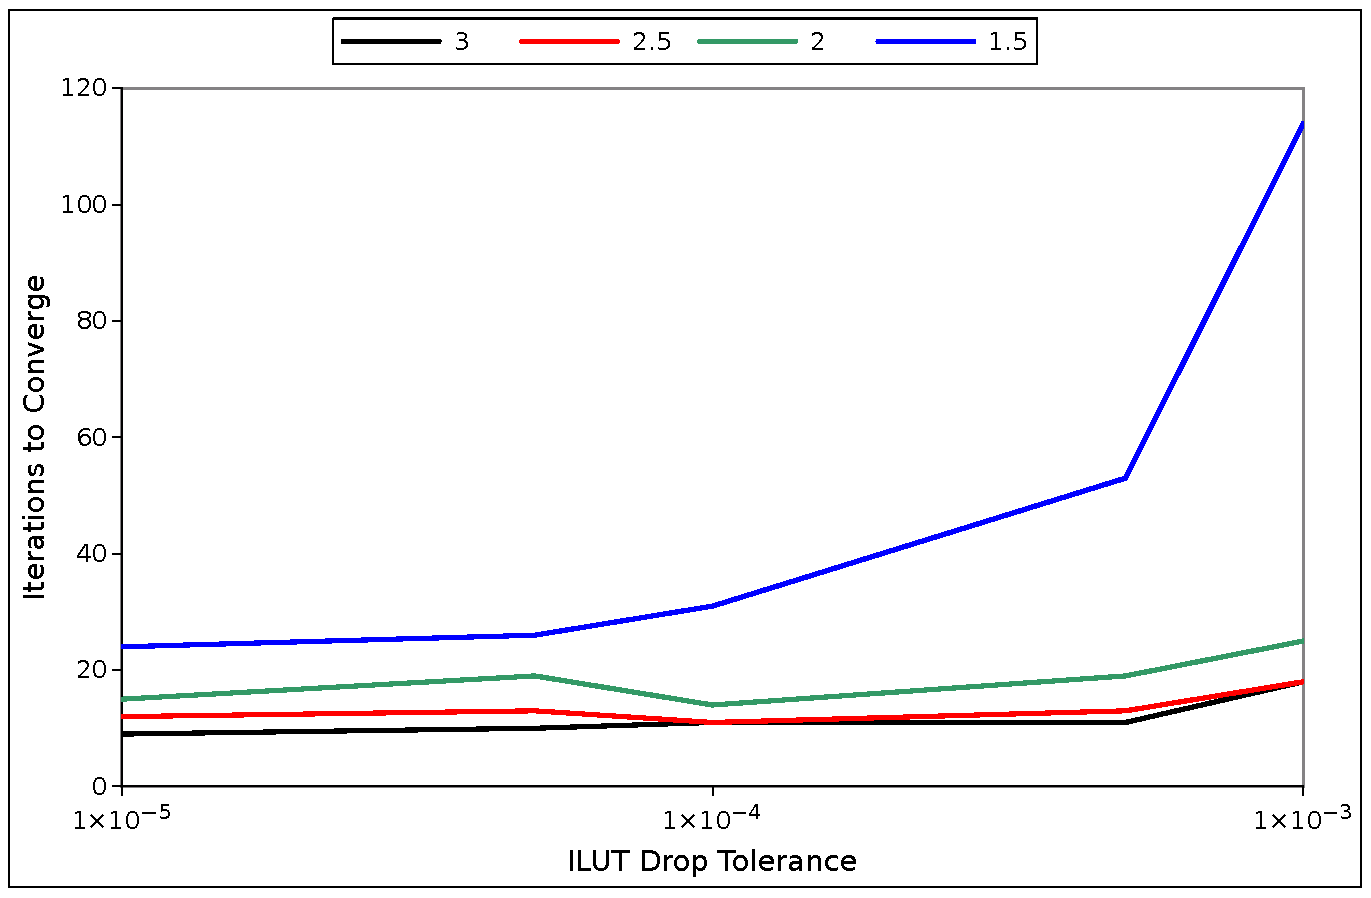
\includegraphics[width=6in]{chapters/spn_equations/ilut_iterations.pdf}
  \end{center}
  \caption{\textbf{Number of MCSA iterations required to converge an
      eigenvalue iteration for the fuel assembly problem with ILUT
      preconditioning as a function of ILUT drop tolerance.}
    \textit{Each colored curve represents the iteration behavior for a
      different ILUT fill level. Fill levels of 1.5, 2.0, 2.5, and 3.0
      were used.}}
  \label{fig:ilut_iterations}
\end{figure}

Unfortunately, gaining convergence (and excellent iterative
performance) with MCSA for the $SP_N$ fuel assembly problem comes at
an immediate cost. Figure~\ref{fig:ilut_size} gives the maximum number
of non-zero entries in the composite linear operator generated by
preconditioning as a function ILUT drop tolerance for varying values
of fill level. For the 1-group $SP_1$ discretization, the original
linear operator will contain only a maximum of 7 non-zero entries per
row in the system. As observed in Figure~\ref{fig:ilut_size},
performing the explicit preconditioning yields composite linear
operators with $O(1,000)$ elements in a row for all combinations of
fill level and drop tolerance, over 10\% of the total row size for
this particular problem. This large number of row entries, observed
for a significant fraction of rows in the system, creates several
problems. First, sparsity is completely destroyed with each state in
the system now coupled to over 10\% of the total states in the system
through the composite iteration matrix. This means that Monte Carlo
sampling tables will be large, requiring significant memory to store
them and a substantial overhead in the sampling procedure during
transport. In addition, the matrix-matrix multiply operations required
to build the composite operator see significant performance losses due
to the amount of data that must be handled. In parallel, losing
sparsity severely inhibits performance where now parallel operations
require communications amongst orders of magnitude more processors for
nearest-neighbor type algorithms.
\begin{figure}[t!]
  \begin{center}
    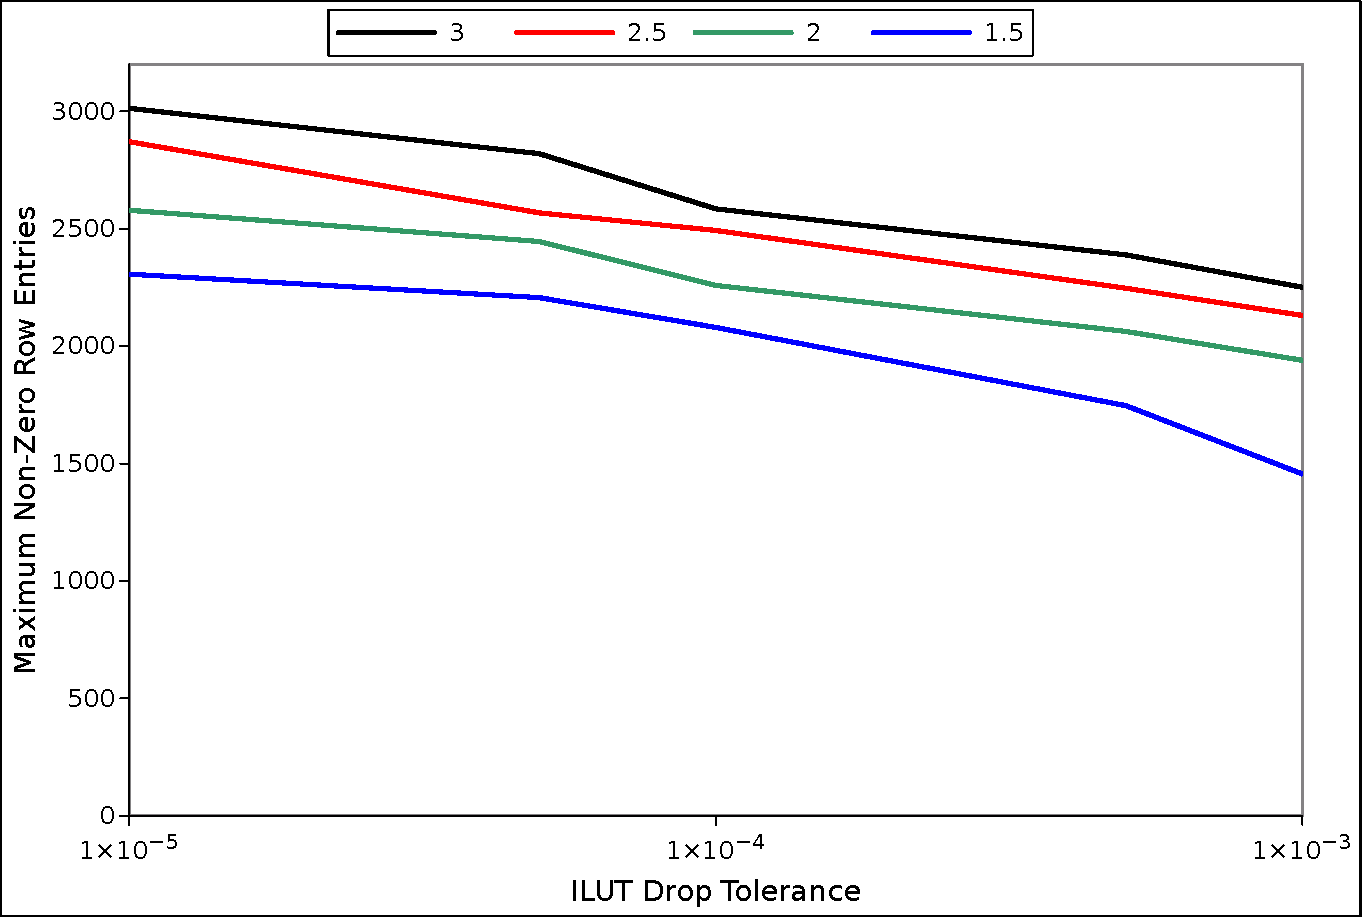
\includegraphics[width=6in]{chapters/spn_equations/ilut_size.pdf}
  \end{center}
  \caption{\textbf{Maximum number of non-zero entries observed for all
      rows in the composite linear operator for the fuel assembly
      problem with ILUT preconditioning given as a function of ILUT
      drop tolerance.} \textit{Each colored curve represents the row
      size for a different ILUT fill level. Fill levels of 1.5, 2.0,
      2.5, and 3.0 were used.}}
  \label{fig:ilut_size}
\end{figure}

As a means to assess the quality of the preconditioning, a simple
metric is developed to address these concerns and allow comparison to
future developments. For our studies, our core performance metric will
be iterative performance with the minimum number of MCSA iterations
required to converge the problem desired. For Monte Carlo
calculations, this improved performance is balanced by the creation of
a dense composite system and we seek to reduce the number of non-zero
entries to a minimum value in order to lower the amount of coupling
amongst states in the system and reduce the amount of memory used
along with the potential latency overhead. Given these two objectives,
the following metric is proposed:
\begin{equation}
  \text{Quality Metric} = (\text{\# iterations}) \times (\text{maximum
    \# of non-zero values})\:,
\end{equation}
where the highest quality preconditioning is one that minimizes this
metric. For the ILUT preconditioned data provided,
Figure~\ref{fig:ilut_quality} provides the computed metric as a
function of ILUT drop tolerance for each fill level used. In general,
the metric is similar to the data observed for the number of
iterations required to converge as the non-zero row entries changed by
a smaller fraction over drop tolerances tested.
\begin{figure}[t!]
  \begin{center}
    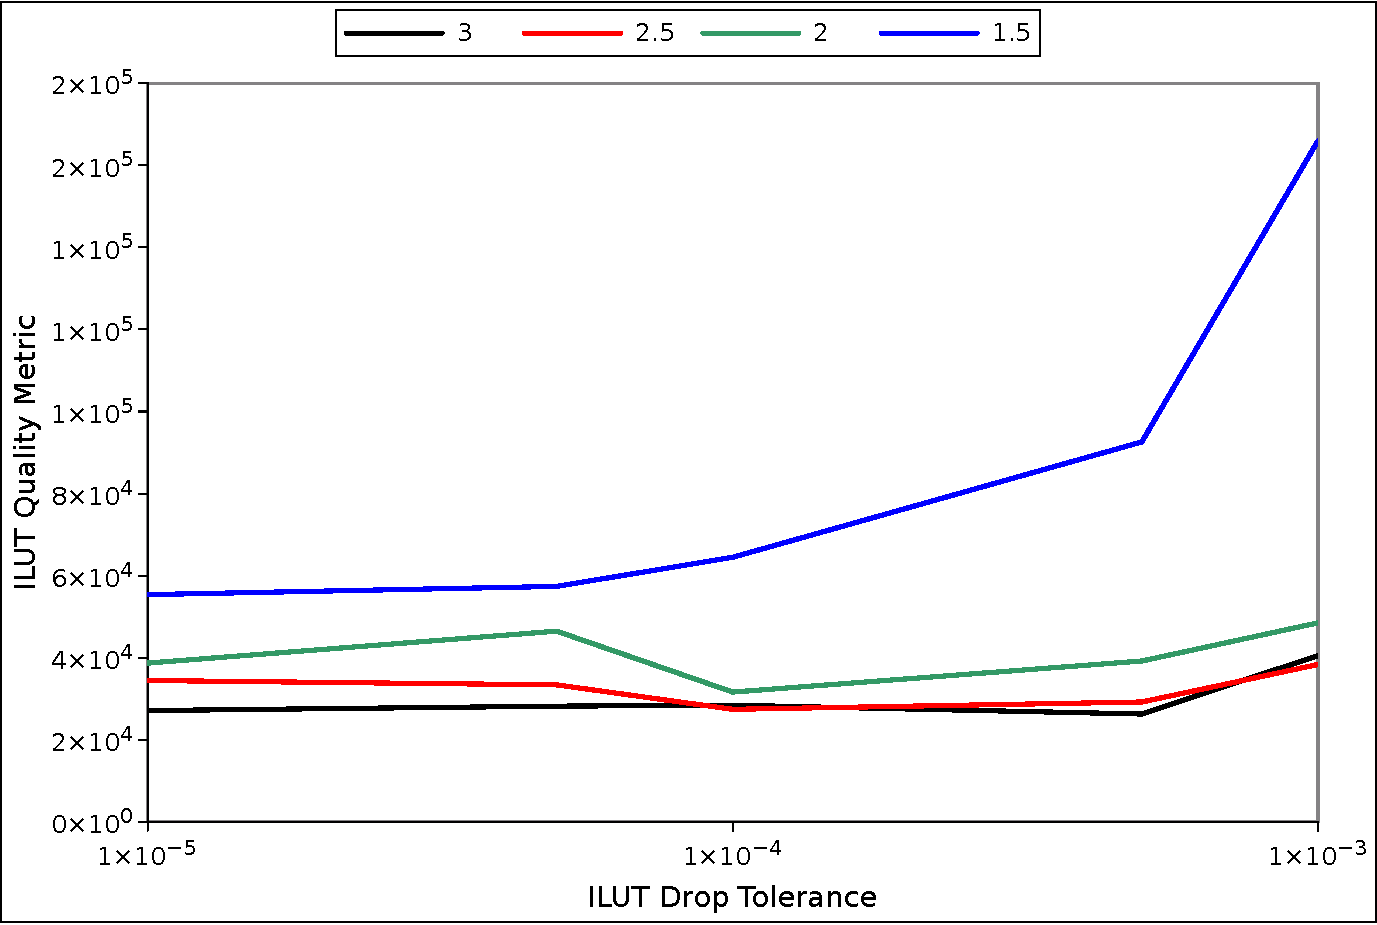
\includegraphics[width=6in]{chapters/spn_equations/ilut_quality.pdf}
  \end{center}
  \caption{\textbf{ILUT preconditioning quality metric for the fuel
      assembly problem given as a function of ILUT drop tolerance.}
    \textit{Each colored curve represents the quality metric behavior
      for a different ILUT fill level. Fill levels of 1.5, 2.0, 2.5,
      and 3.0 were used.}}
  \label{fig:ilut_quality}
\end{figure}

It should be noted here that although only the behavior of the linear
solve during a single eigenvalue iteration is reported, the behavior
of the linear solver was observed to be consistent throughout the
eigenvalue iterations (25 total eigenvalue iterations were required to
converge the 1-group $SP_1$ problem). We expect this as the linear
operator (which is unchanging in the fuel assembly criticality
problem) dictates the convergence of MCSA. At each iteration the
fission source provided to the linear problem is changing, however, we
expect the same convergence behavior for all source vectors
$\mathbf{b} \in \mathbb{R}^{N}$ where $||\mathbf{b}||_1 \neq 0$.

\subsection{Sparse Approximate Inverse Preconditioning}
\label{subsec:spn_spainv_preconditioning}
Explicit formation of the preconditioner inverse is a requirement of
the current MCSA preconditioning strategy. As a result, although ILUT
preconditioning provided excellent iterative performance, a
significant time penalty is paid to extract the inverse of the
triangular factors through $N$ triangular solves. In addition, this
explicit inversion yielded a composite linear operator that was dense,
requiring modification of the system in order to achieve better
scalability and Monte Carlo performance. Sparse approximate inverse
(SPAINV) preconditioning is a technique that may potentially alleviate
both of these constraints at the cost of reduced iterative
performance. The method produces a sparse approximation of the inverse
matrix directly by minimizing the Frobenius norm of the residual
matrix \citep{saad_iterative_2003}:
\begin{equation}
  || \mathbf{I} - \mathbf{A} \mathbf{M} ||^2_F =
  \sum_{j=1}^N ||\mathbf{e}_j - \mathbf{A} \mathbf{m}_j||^2_2 \:,
  \label{eq:frobenius_norm_min}
\end{equation}
where the inverse preconditioning matrix $\mathbf{M}$ minimizes the
norm on the right and $\mathbf{e}_j$ and $\mathbf{m}_j$ are the
$j^{th}$ columns of the identity and preconditioning matrices
respectively. Here, $\mathbf{M}$ is the actual inverse of the
preconditioner and is formed directly by the algorithm. On the right
hand side of Eq~(\ref{eq:frobenius_norm_min}), the Frobenius norm is
represented as a effective sum of $N$ linear system residual norms. A
few iterations of a subspace method or other iterative scheme can be
used to effectively solve these systems to a loose tolerance and yield
the columns of the approximate preconditioning matrix. At each
iteration, threshold values are used to eliminate the components of
each $\mathbf{m}_j$ column to maintain the desired level of
sparsity. In addition, a sparsity pattern can be predetermined and
enforced during this process. For the SPAINV implementation used for
this work, the sparsity pattern was defined by levels such that a
level of $N$ for an input operator $\mathbf{A}$ will generate a
preconditioning matrix $\mathbf{M}$ with the same sparsity pattern as
$\mathbf{A}^{N+1}$. By using the norm minimization strategy instead of
a factorization such as ILUT, parallel results are reproduced
regardless of parallel problem size, meaning that a serial computation
will converge in the same number of iterations as a computation with
thousands of cores.

MCSA preconditioned with SPAINV was used to solve the fuel assembly
problem as with ILUT for a 1-group $SP_1$ discretization. To study
convergence sensitivity to SPAINV parameters, the number of levels in
the sparsity pattern and threshold were parametrically varied with the
number of iterations to converge a single eigenvalue iteration for the
fuel assembly problem recorded along with the maximum number of
non-zero entries observed in all matrix rows for the left/right
preconditioned composite linear operator. For each calculation, the
number of iterations required to converge reported was for a single
eigenvalue iteration with \sn{3}{4} histories at each MCSA iteration
to compute the Monte Carlo correction using the adjoint collision
estimator. All SPAINV calculations reported here were performed on a
single CPU.

Figure~\ref{fig:spainv_iterations} gives the number of MCSA iterations
needed to converge the fuel assembly problem and
Figure~\ref{fig:spainv_size} the maximum number of non-zero entries
per row obeserved in the composite linear operator as a function the
SPAINV threshold. For this analysis, the number of levels in the
sparsity pattern was varied from 3 to 7 with convergence of the fuel
assembly problem not achieved for smaller level values. Compared to
ILUT preconditioning, at higher levels we see comparable iterative
performance with a relative invariance to the threshold value. The
threshold did have a significant effect, however, on the time required
to generate the preconditioner with a threshold of 0.001 over an order
of magnitude slower than a threshold of 0.01 due to the inclusion of a
significant number of extra values in the input operator. In addition
to comparable iterative performance, the sparsity of the composite
operator is greatly improved with nearly an order of magnitude
reduction in number of non-zero entries per row for lower level
values.
\begin{figure}[t!]
  \begin{center}
    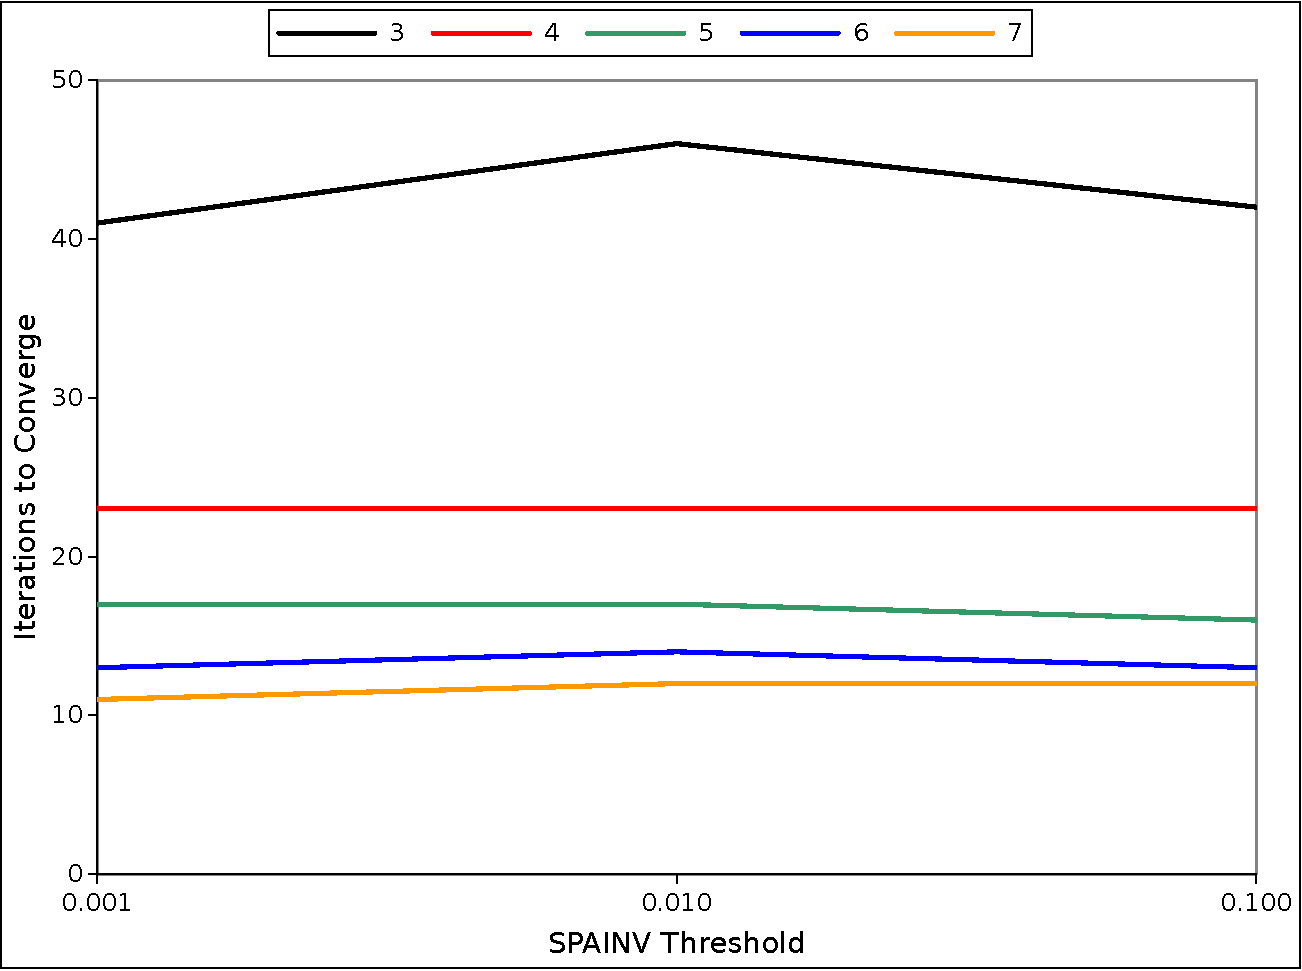
\includegraphics[width=6in]{chapters/spn_equations/spainv_iterations.pdf}
  \end{center}
  \caption{\textbf{Number of MCSA iterations required to converge a
      single eigenvalue iteration for the fuel assembly problem with
      SPAINV preconditioning as a function of SPAINV threshold.}
    \textit{Each colored curve represents the iteration behavior for a
      different SPAINV level pattern. Levels of 3, 4, 5, 6, and 7 were
      used.}}
  \label{fig:spainv_iterations}
\end{figure}
\begin{figure}[t!]
  \begin{center}
    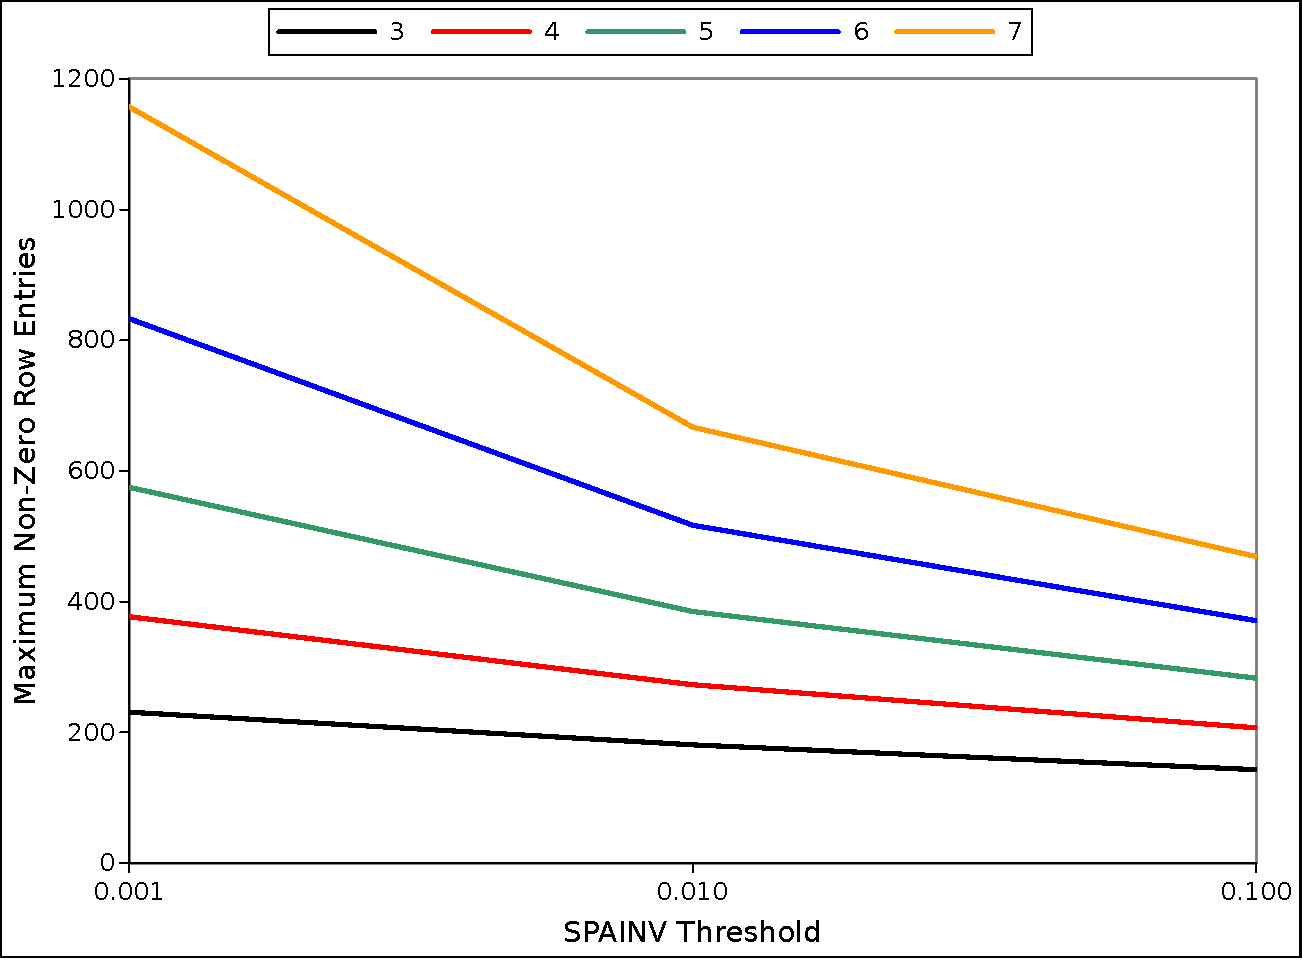
\includegraphics[width=6in]{chapters/spn_equations/spainv_size.pdf}
  \end{center}
  \caption{\textbf{Maximum number of non-zero entries observed for all
      rows in the composite linear operator for the fuel assembly
      problem with SPAINV preconditioning given as a function of
      SPAINV threshold.} \textit{Each colored curve represents the row
      size for a different SPAINV level pattern. Levels of 3, 4, 5, 6,
      and 7 were used.}}
  \label{fig:spainv_size}
\end{figure}

With the comparable iterative performance and improved sparsity,
SPAINV preconditioning should then have a more favorable quality
metric than ILUT preconditioning. Figure~\ref{fig:spainv_quality}
gives the quality metric as a function of the threshold value for each
of the sparsity levels computed. Not only do we see an improved
quality metric over ILUT preconditioning (about an order of magnitude
less), but we also note that the ideal sparsity level is not the largest
nor the smallest. In fact, the largest and smallest levels (3 and 7)
performed the worst in terms of the quality metric with a level of 4
performing the best. When CPU time to generate the preconditioner is
considered, 4 is the clear choice for this problem as more time is
required to do the approximate inversion as the sparsity pattern of
the preconditioner grows in size.
\begin{figure}[t!]
  \begin{center}
    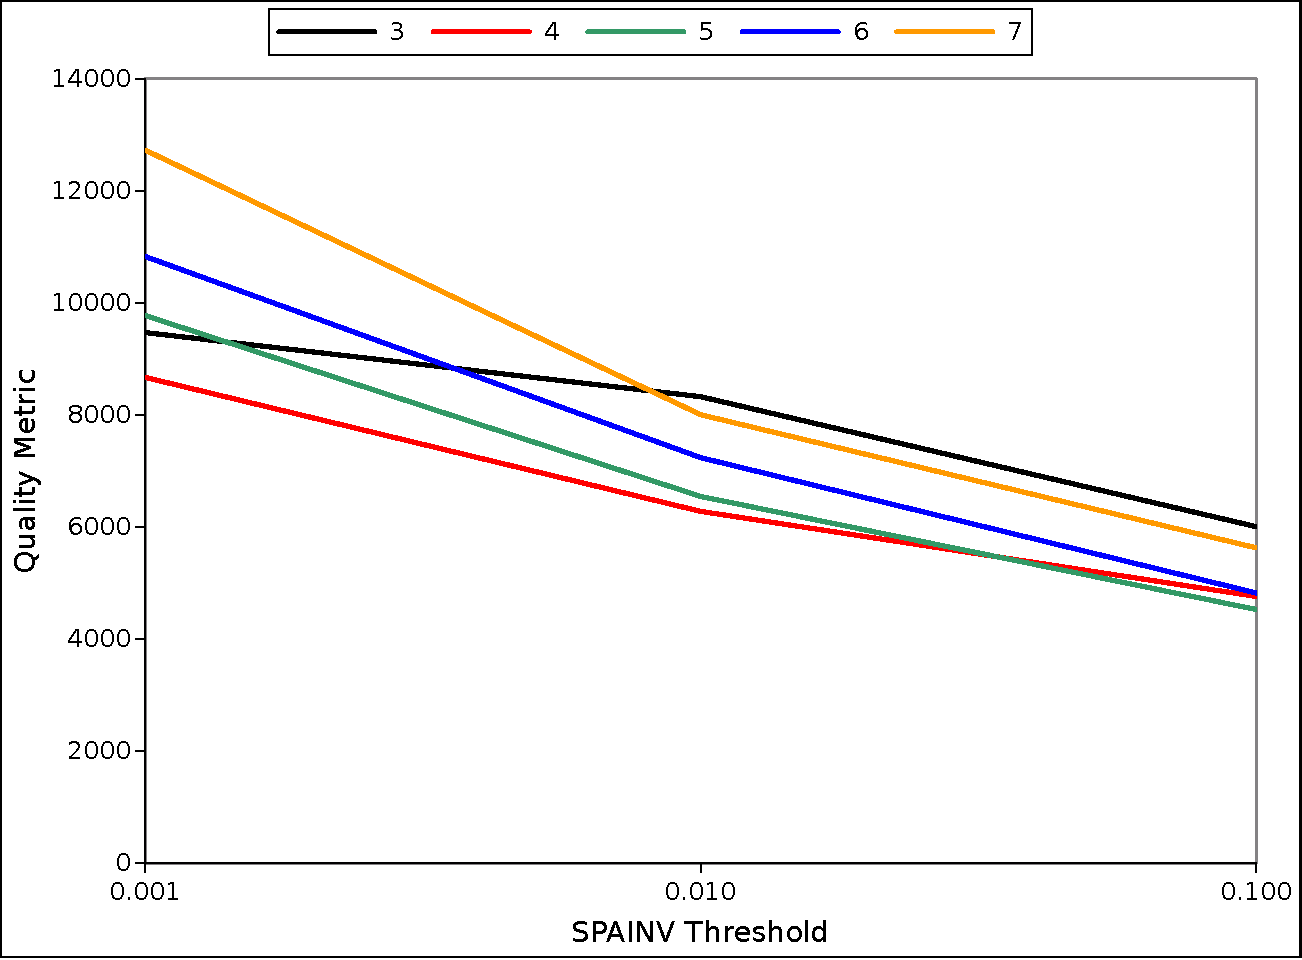
\includegraphics[width=6in]{chapters/spn_equations/spainv_quality.pdf}
  \end{center}
  \caption{\textbf{SPAINV preconditioning quality metric for the fuel
      assembly problem given as a function of SPAINV threshold.}
    \textit{Each colored curve represents the quality metric behavior
      for a different SPAINV level pattern. Levels of 3, 4, 5, 6, and
      7 were used.}}
  \label{fig:spainv_quality}
\end{figure}

\clearpage

\subsection{SPAINV Improved ILUT Preconditioning}
\label{subsec:spn_spainv_preconditioning}
As a means to improve convergence over using only SPAINV
preconditioning, ILUT preconditioning may be modified through an
additional application of SPAINV
(SPAINV-ILUT)\citep{saad_iterative_2003}. For the ILUT preconditioning
case we have the following linear problem to solve for the substituted
variable:
\begin{equation}
  \mathbf{L}^{-1} \mathbf{A} \mathbf{U}^{-1} \mathbf{u} =
  \mathbf{L}^{-1} \mathbf{b}\:.
  \label{eq:ilut_standalone}
\end{equation}
We then apply SPAINV and minimize the following problem, this time on
the left:
\begin{equation}
  || \mathbf{I} - \mathbf{M} \mathbf{L}^{-1} \mathbf{A}
  \mathbf{U}^{-1} ||^2_F\:,
  \label{eq:ilut_minimize}
\end{equation}
giving a new preconditioned system:
\begin{equation}
  \mathbf{M} \mathbf{L}^{-1} \mathbf{A} \mathbf{U}^{-1} \mathbf{u} =
  \mathbf{M} \mathbf{L}^{-1} \mathbf{b}\:.
  \label{eq:ilut_spainv}
\end{equation}
Doing this permits a smaller fill level to be used with ILUT and a
lower-order sparsity pattern to be used with SPAINV, giving marginally
more sparsity in the resulting composite linear operator while
maintaining good iterative performance.

MCSA preconditioned with SPAINV-ILUT was also used to solve the same
fuel assembly problem as with the other preconditioners for the same
1-group $SP_1$ discretization. To study convergence sensitivity to
SPAINV-ILUT parameters, the ILUT drop tolerance and ILUT fill level
were parametrically varied with the number of iterations to converge a
single eigenvalue iteration for the fuel assembly problem recorded
along with the maximum number of non-zero entries observed in all
matrix rows for the left/right preconditioned composite linear
operator. SPAINV parameters for the data presented here were fixed as
it was found that the preconditioning quality was largely insenstive
to their variation. In addition, the fact that SPAINV is being used to
preconditioned a problem already preconditioned with ILUT means that
the input matrix sparsity pattern is already somewhat dense and large
SPAINV levels would result in an even denser system. Therefore, a
smaller SPAINV sparsity pattern level will be used for this
preconditioning. For each calculation, the number of iterations
required to converge reported was for a single eigenvalue iteration.
Again, \sn{3}{4} histories are used at each MCSA iteration to compute
the Monte Carlo correction using the adjoint collision estimator. All
SPAINV-ILUT calculations reported here were performed on a single CPU.

Figure~\ref{fig:spainv_ilut_iterations} gives the number of iterations
required to converge as a function of ILUT drop tolerance for ILUT
fill levels of 1.5, 2.0, 3.0, 4.0 and 5.0 with a fixed SPAINV
threshold of 1.0 and sparsity level of 1. SPAINV threshold values
higher than 1.0 resulted in a loss of convergence and lower values did
not significantly affect performance. Larger sparsity levels resulted
in a composite operator that was too dense and a prohibitive amount of
CPU time required to compute the preconditioner. At smaller levels of
fill, the benefits of using an additional step of SPAINV
preconditioning are readily observed with the number of iterations
required to converge cut in half for large drop tolerances. For
smaller drop tolerances and higher ILUT levels of fill, the additional
step of SPAINV preconditioning offers marginal improvement to
iterative performance. As shown in Figure~\ref{fig:spainv_ilut_size},
because ILUT is used in the preconditioning sequence, sparsity is
again lost with only marginally improved non-zero entry numbers due to
the application of the SPAINV threshold. As a result, the quality
metrics given by Figure~\ref{fig:spainv_ilut_quality} are only
marginally better than those observed for ILUT preconditioning and
much larger than the SPAINV quality metric values.
\begin{figure}[t!]
  \begin{center}
    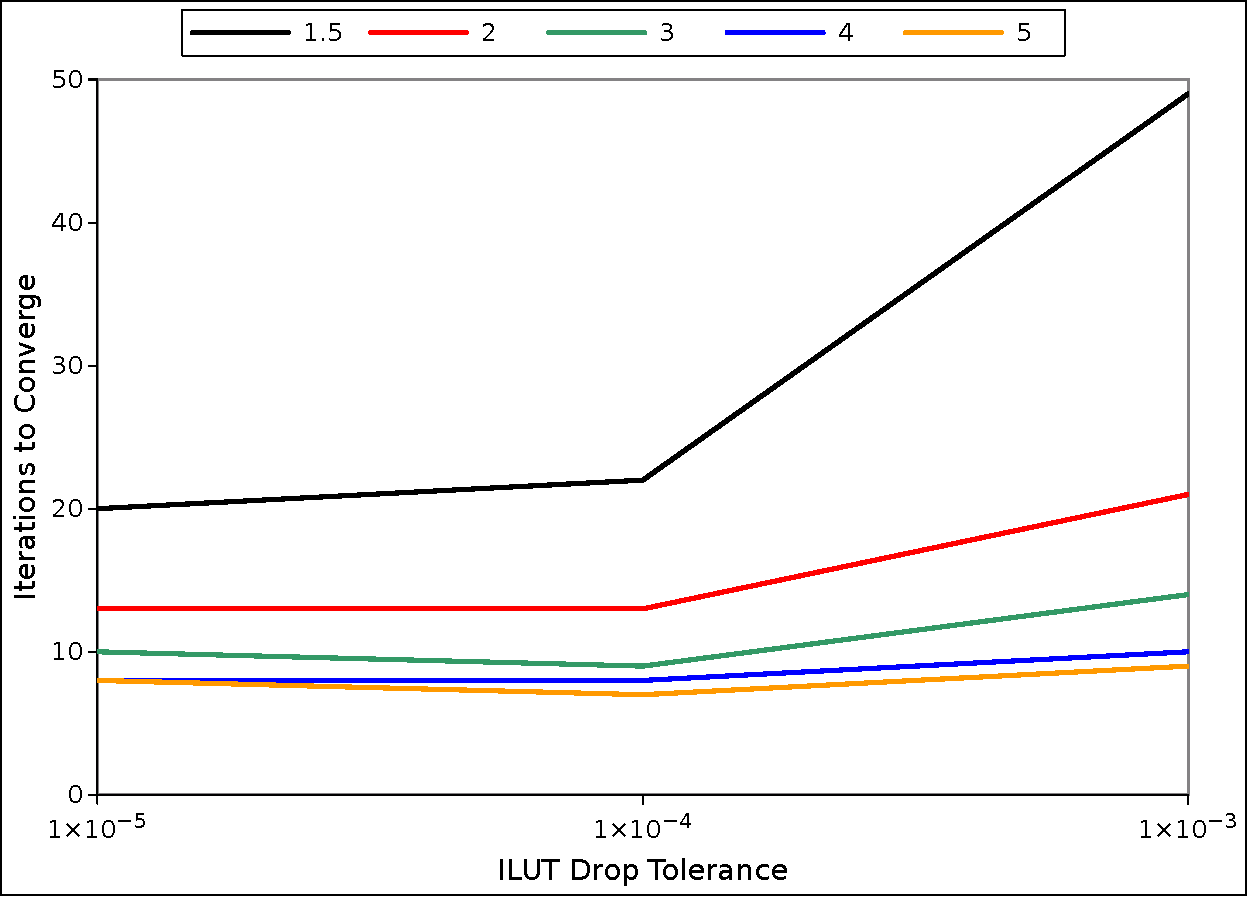
\includegraphics[width=6in]{chapters/spn_equations/psilut_iterations.pdf}
  \end{center}
  \caption{\textbf{Number of MCSA iterations required to converge a
      single eigenvalue iteration for the fuel assembly problem with
      SPAINV-ILUT preconditioning as a function of ILUT drop
      tolerance.} \textit{Each colored curve represents the row size
      for a different ILUT fill level. Fill levels of 1.5, 2.0, 3.0,
      4.0, and 5.0 were used.}}
  \label{fig:spainv_ilut_iterations}
\end{figure}

\begin{figure}[t!]
  \begin{center}
    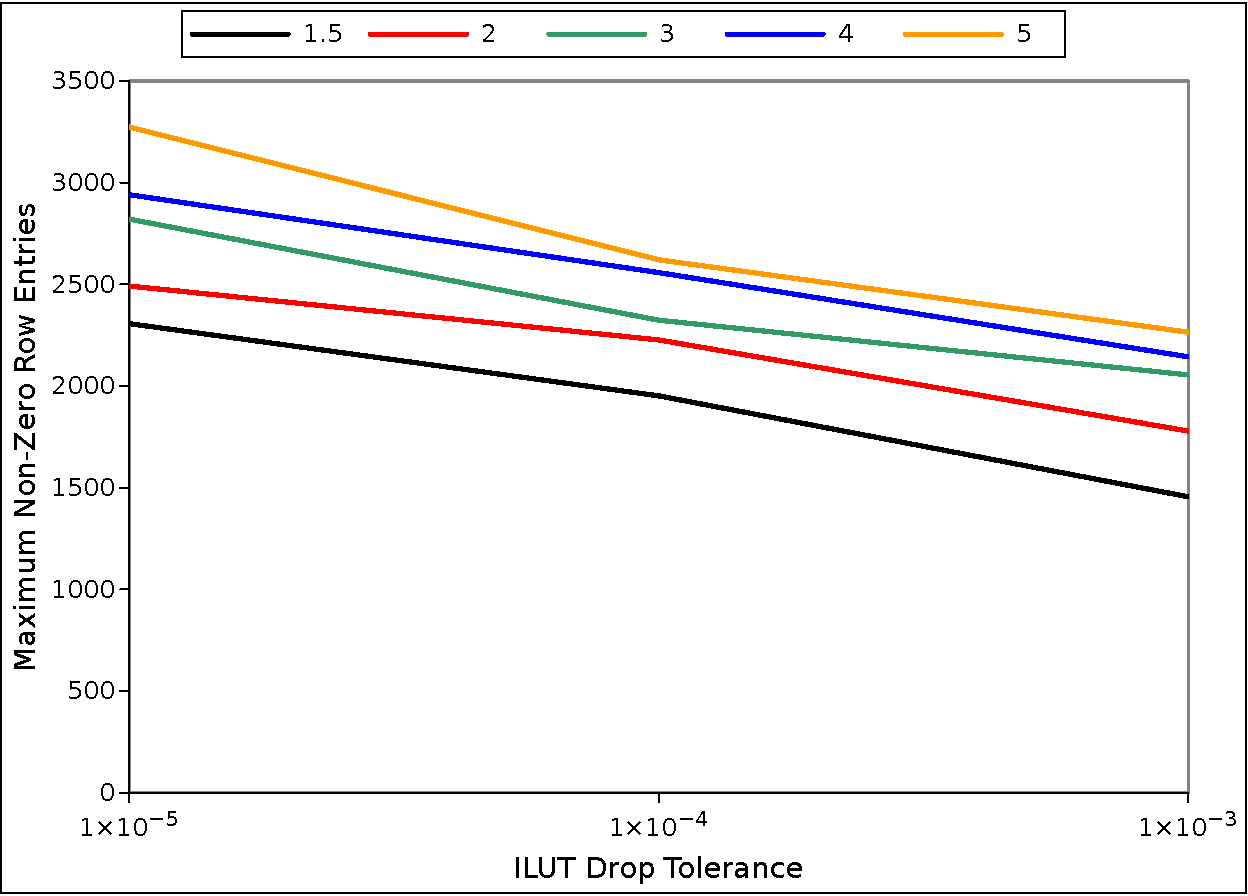
\includegraphics[width=6in]{chapters/spn_equations/psilut_size.pdf}
  \end{center}
  \caption{\textbf{Maximum number of non-zero entries observed for all
      rows in the composite linear operator for the fuel assembly
      problem with SPAINV-ILUT preconditioning given as a function of
      ILUT drop tolerance.} \textit{Each colored curve represents the
      row size for a different ILUT fill level. Fill levels of 1.5,
      2.0, 3.0, 4.0 and 5.0 were used.}}
 \label{fig:spainv_ilut_size}
\end{figure}

\begin{figure}[t!]
  \begin{center}
    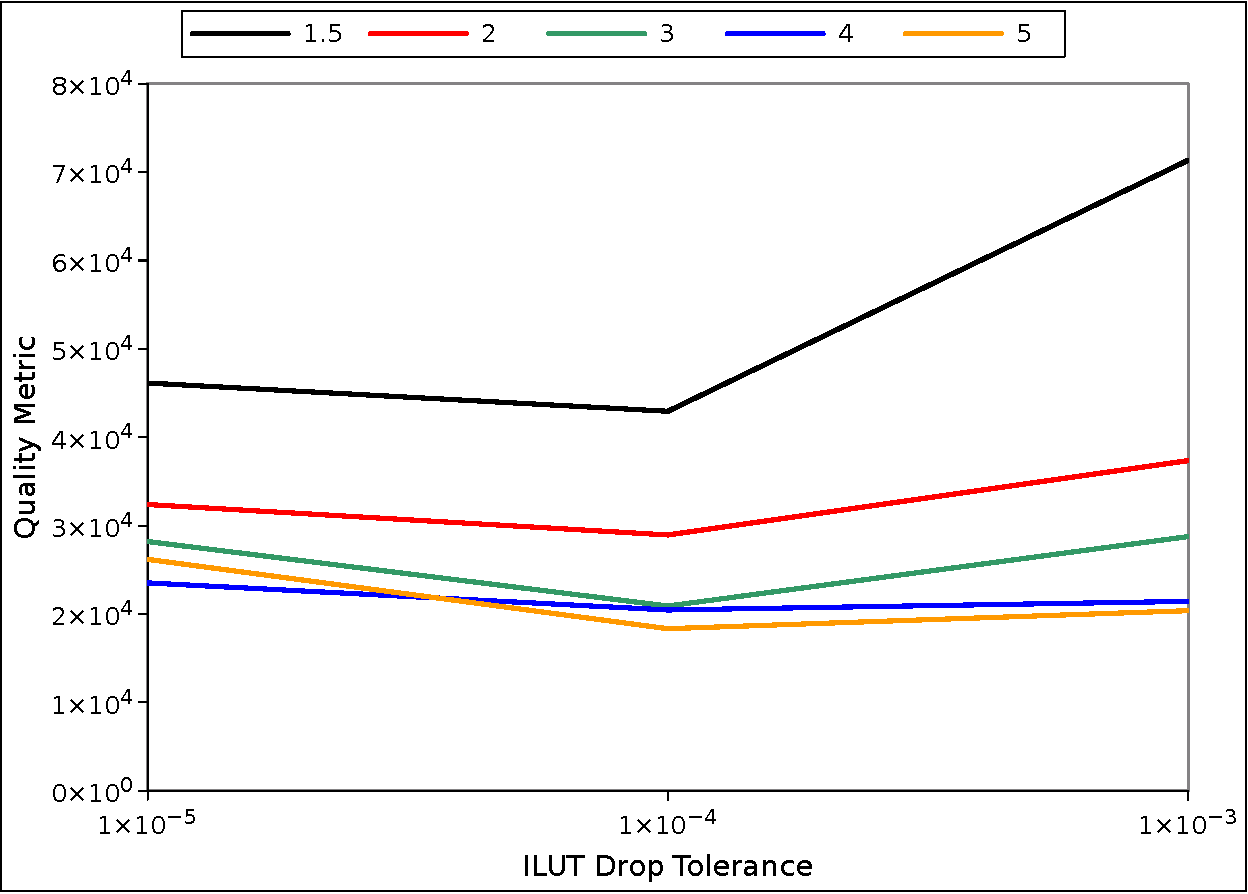
\includegraphics[width=6in]{chapters/spn_equations/psilut_quality.pdf}
  \end{center}
  \caption{\textbf{SPAINV-ILUT preconditioning quality metric for the
      fuel assembly problem given as a function of ILUT drop
      tolerance.} \textit{Each colored curve represents the row size
      for a different ILUT fill level. Fill levels of 1.5, 2.0, 3.0,
      4.0 and 5.0 were used.}}
  \label{fig:spainv_ilut_quality}
\end{figure}

\clearpage

\subsection{Applying the Reduced Domain Approximation}
\label{subsec:spn_prec_rda}
For each preconditioning technique presented convergence was achieved
for the single fuel assembly problem. However, a primary concern is
the number of non-zero states in each row of the system generated by
the explicit preconditioning strategy. In many cases, orders of
magnitude more matrix elements were generated resulting in poor
scalability for domain decomposed algorithms and overall performance
issues for Monte Carlo. As outlined in
\S~\ref{subsec:reduced_domain_approximation}, the reduced domain
approximation may be used as a mechanism to potentially alleviate this
problem by filtering elements of the composite matrix in each row that
fall below a certain threshold value or by maintaining the largest $N$
elements in each row where $N$ is a designated fill level.

For the ILUT, SPAINV, and SPAINV-ILUT preconditioning strategies the
reduced domain approximation will be applied to reduce the density of
the composite linear operator to more manageable levels. For each
preconditioner, the parameters that achieved the best quality metric
results from the previous analysis were used. These correspond to ILUT
parameters of a fill level of 5.0 and a drop tolerance of \sn{1}{-5},
SPAINV parameters of a sparsity level of 4 and a threshold of 0.1 and
SPAINV-ILUT with ILUT parameters of a fill level of 4.0 and a drop
tolerance of \sn{1}{-5} and SPAINV parameters of a sparsity level of 1
and a threshold of 1.0. The reduced domain threshold was set to
\sn{1}{-10} in order to eliminate any exceedingly small values from
the matrix (generally this is simply removing non-zero elements within
the floating point tolerance of zero). The reduced domain fill level
was then varied, starting with the largest non-zero entries per row
value observed for each of the preconditioning types in order to
assess its effects relative to the case where no reduced domain
approximation was applied.

Figure~\ref{fig:rda_iterations} gives the number of iterations
required to converge for each preconditioner type as a function of
reduced domain fill level. Figure~\ref{fig:rda_quality} gives the
corresponding quality metric for each data point where the number of
non-zero entries used to compute the metric is equivalent to the
reduced domain fill level. We first note the SPAINV preconditioning
alone is signficantly more sensitive to the reduction in domain size
over the ILUT-based methods, although the preconditioner was of
$O(100)$ non-zero entries per row without any approximation
applied. For the ILUT-based methods, performance was significantly
better with convergence achieved in less than 40 MCSA iterations with
only 10 non-zero entries in each row (vs. 7 non-zero entries for the
case with no preconditioning). SPAINV-ILUT iterative performance was
marginally better than ILUT alone for all reduced domain fill
levels. However, it should be noted that the ILUT level of fill used
for the ILUT only calculations was set to 4 for this case while the
SPAINV-ILUT preconditioner used an ILUT level of fill of 5 and
therefore the marginally better performance is more likely a result of
this addition of fill rather than the extra SPAINV
preconditioning. Looking at the quality metric data, we see a nice
power-law reduction in the quality metric as a function of the reduced
domain fill level, achieving 2 orders of magnitude reduction in the
quality metric for the ILUT-based preconditioning methods.

Although applying the reduced domain approximation results in a
successful recovery of sparsity for the Monte Carlo problem while
maintaining good convergence properties, there is still an issue of
forming the composite operator before applying the approximation and
potentially generating the transpose of this operator in the case of
the adjoint Monte Carlo method. Because of this, memory and scaling
issues may still be observed when building the probability and weight
matrices for the Monte Carlo problem. In addition, the expensive
extraction of the inverse of the preconditioning operators for the
explicit scheme creates a significant cost in overall
performance. Future work in this area should be considerate of these
important components of the preconditioned MCSA algorithm.

\begin{figure}[t!]
  \begin{center}
    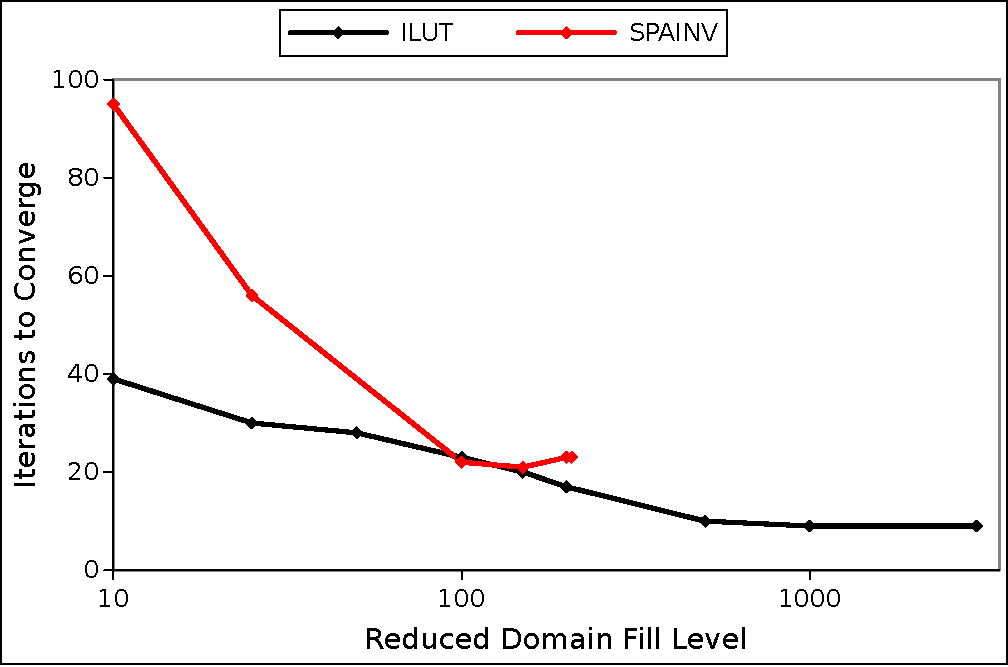
\includegraphics[width=6in]{chapters/spn_equations/rda_iterations.pdf}
  \end{center}
  \caption{\textbf{Number of MCSA iterations required to converge a
      single eigenvalue iteration for the fuel assembly problem with
      each preconditioning as a function of reduced domain
      approximation fill level.} \textit{The largest fill level for
      each preconditioning presented is that using the parameters that
      gave the best results without the approximation.}}
  \label{fig:rda_iterations}
\end{figure}

\begin{figure}[t!]
  \begin{center}
    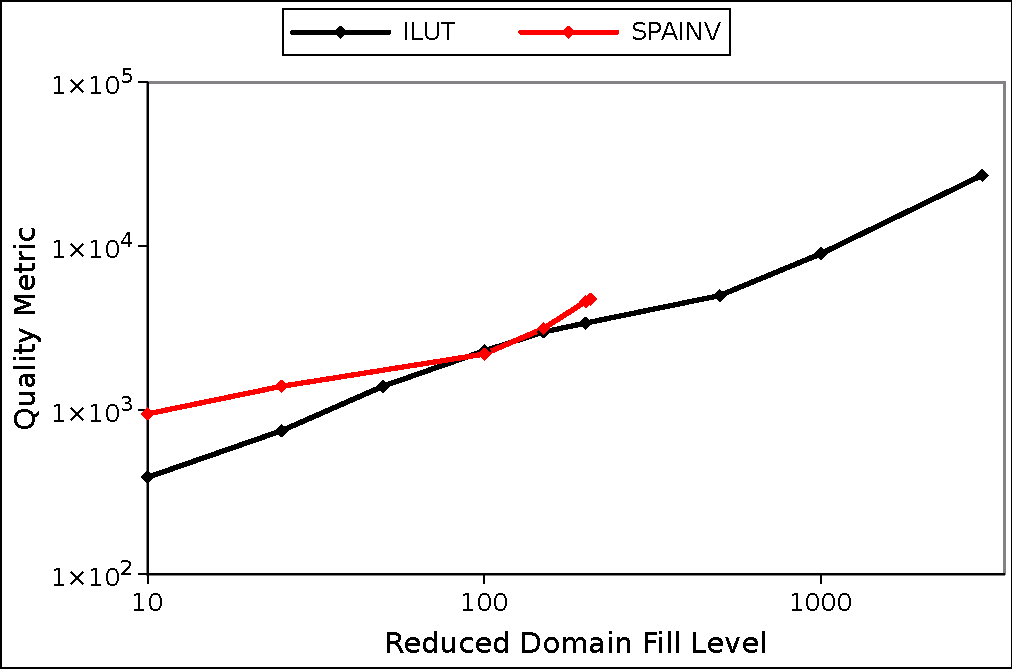
\includegraphics[width=6in]{chapters/spn_equations/rda_quality.pdf}
  \end{center}
  \caption{\textbf{Preconditioning quality metric for the fuel
      assembly problem given as a function of reduced domain
      approximation fill level.} \textit{The largest fill level for
      each preconditioning presented is that using the parameters that
      gave the best results without the approximation.}}
  \label{fig:rda_quality}
\end{figure}

\clearpage

\subsection{MCSA Relaxation Parameters}
\label{subsec:spn_mcsa_relaxation}
The Richardson iteration upon which the Neumann-Ulam method is built
may be implemented with a scalar relaxation parameter that can be
adjusted to improve convergence:
\begin{equation}
  \mathbf{x} = \mathbf{x} + \omega \mathbf{r}\:,
  \label{eq:richardson_relaxation}
\end{equation}
where $\omega$ is the relaxation parameter. This is effectively a form
of preconditioning where the system is being scaled on the left by a
constant value in all rows. Analogously, these relaxation parameter
techniques can be applied to Monte Carlo to improve convergence as
demonstrated by Dimov \citep{dimov_new_1998}. In this case, building
an iteration matrix from Eq~(\ref{eq:richardson_relaxation}) gives:
\begin{equation}
  \mathbf{H} = \mathbf{I} - \omega \mathbf{A}\:,
  \label{eq:relaxed_iteration_matrix}
\end{equation}
with the probabilities and weights for the Monte Carlo procedure
appropriately scaled. By inspection, such a scaling is a simple form
of preconditioning on the left where all rows in the system are scaled
by the same scalar parameter. For MCSA, we can stage this scheme with
two separate relaxation parameters; one for the outer Richardson
iteration and one for the inner Monte Carlo solve:
\begin{subequations}
  \begin{gather}
    \ve{x}^{k+1/2} = \ve{x}^k + \omega_R \ve{r}^k\:,\\ \ve{r}^{k+1/2}
    = \ve{b} -
    \ve{A}\ve{x}^{k+1/2}\:,\\ \omega_N\ve{A}\delta\ve{x}^{k+1/2} =
    \omega_N\ve{r}^{k+1/2}\:,\\ \ve{x}^{k+1} = \ve{x}^{k+1/2} + \delta
    \ve{x}^{k+1/2}\:,\\ \ve{r}^{k+1} = \ve{b} - \ve{A}\ve{x}^{k+1}\:,
  \end{gather}
  \label{eq:mcsa_relaxed}
\end{subequations}
where $\omega_R$ is the Richardson iteration relaxation parameter and
$\omega_N$ is the Neumann-Ulam Monte Carlo solve relaxation parameter.

We apply these relaxation parameters to the fuel assembly problem
along with the reduced domain approximation as a means of studying
their effects. For each calculation presented, the number of
iterations required to converge reported was for a single eigenvalue
iteration.  Again, \sn{3}{4} histories are used at each MCSA iteration
to compute the Monte Carlo correction using the adjoint collision
estimator. A reduced domain fill level of 100 is used with a threshold
of \sn{1}{-10} to filter small values. ILUT preconditioning with a
drop tolerance of \sn{1}{-5} and fill level of 5 is used as
well. 

Figure~\ref{fig:relax_iters} gives the number of iterations required
to converge the fuel assembly problem for a 1-group SP1 discretization
using varying combinations of the relaxation parameters. First, both
parameters were fixed at the base case of 1 while the other parameter
was varied as shown in the left-hand side plots of
Figure~\ref{fig:relax_iters}. For the Richardson relaxation parameter,
using a value larger than 1 gave better iterative performance up to a
point, effectively providing a stronger extrapolation using the
residual at each iteration. For the Neumann relaxation parameter, a
value of less than 1 is observed to be ideal. Although initially
counter-intuitive, the fact that the correction computed by the Monte
Carlo solver has a stochastic error associated with it means that by
using a Neumann relaxation parameter less than 1, the correction and
its error are effectively dampened to improve iterative
performance. Considering the CPU time required to converge a single
eigenvalue iteration, similar results are also observed for the
relaxation parameters as given by Figure~\ref{fig:relax_time}. For the
base cases given by the plots on the left, it was found the a
Richardson relaxation parameter of 1.1 and a Neumann relaxation
parameter of 0.7 provided the fastest CPU time for convergence. Fixing
each parameter at these new values, the calculations were repeated as
shown for the plots on the right hand sides of both
Figures~\ref{fig:relax_iters} and \ref{fig:relax_time}. For each
repeated timing calculation, it was found that the same combination of
relaxation parameters found in the base cases performed the best
although they did not necessarily have the best iterative performance.

\begin{figure}[t!]
  \begin{center}
    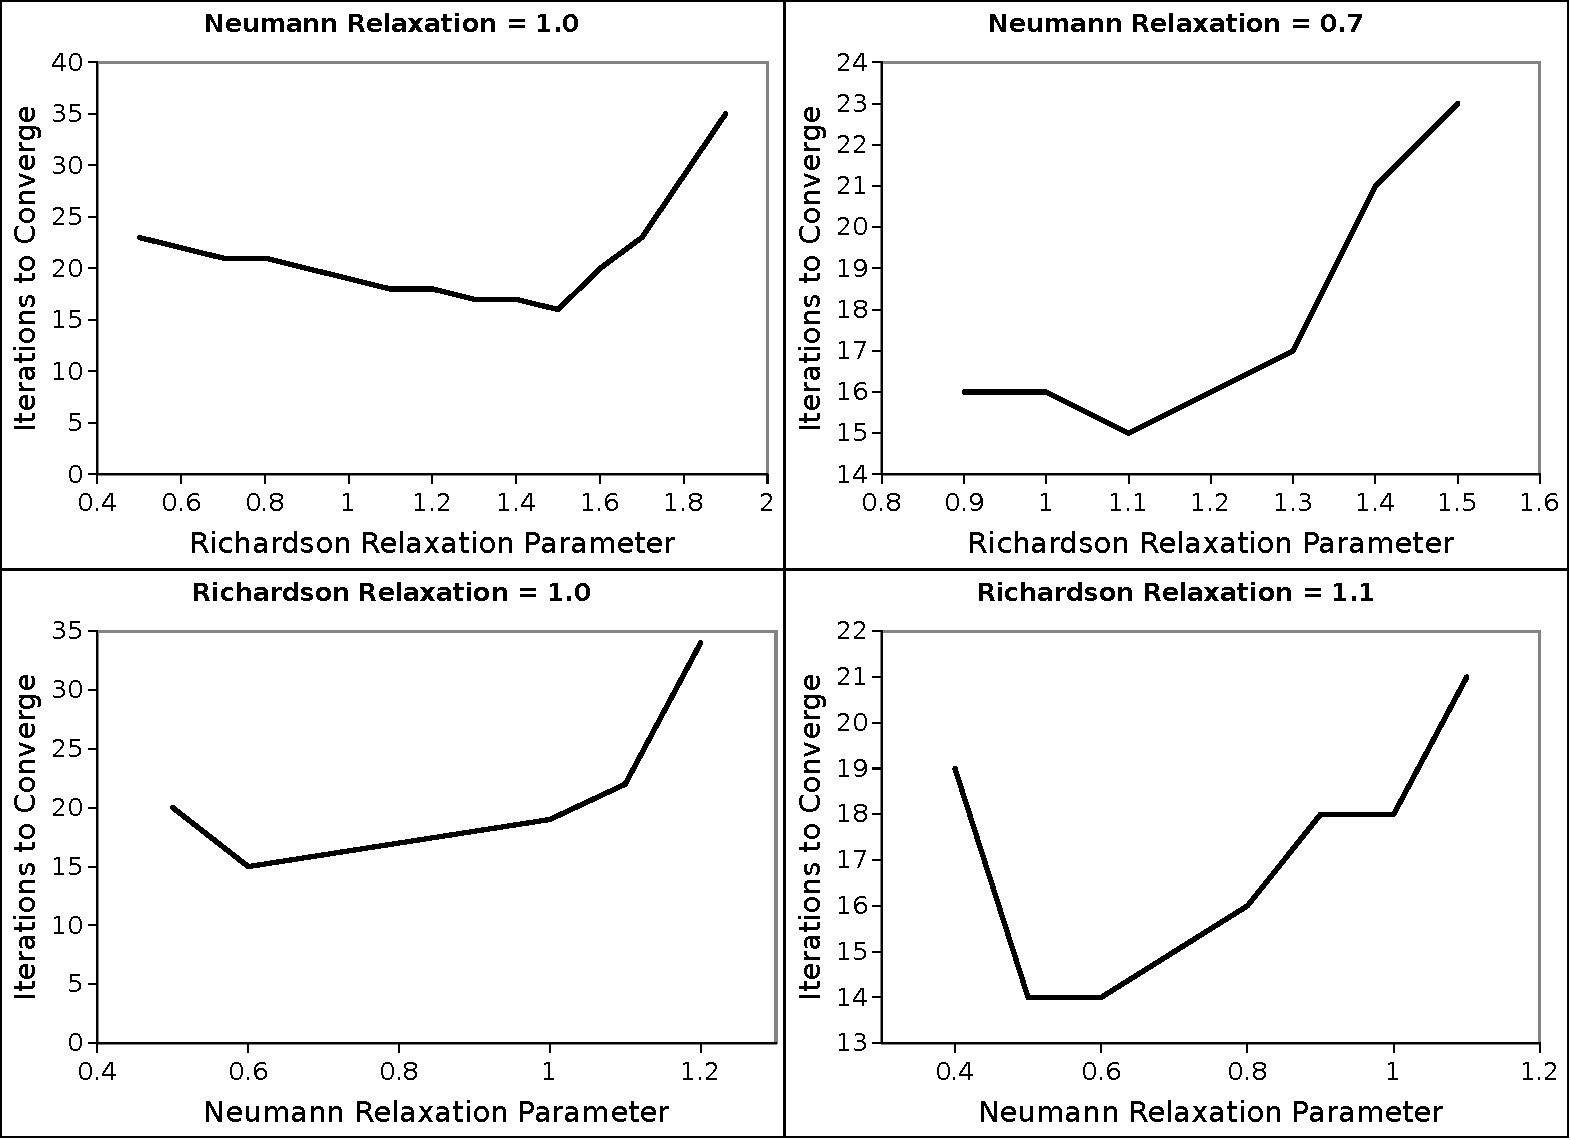
\includegraphics[width=6in]{chapters/spn_equations/relax_iters.pdf}
  \end{center}
  \caption{\textbf{Number of iterations to converge a single
      eigenvalue iteration of the fuel assembly problem as a function
      of the relaxation parameters.} \textit{Starting in upper left
      and moving counter-clockwise: Neumann relaxation parameter fixed
      at 1.0, Richardson relaxation parameter fixed at 1.0, Neumann
      relaxation parameter fixed at 0.7, Richardson relaxation
      parameter fixed at 1.1. For each calculation \sn{3}{4}
      stochastic histories were used to compute the MCSA correction at
      each iteration.}}
  \label{fig:relax_iters}
\end{figure}

\begin{figure}[t!]
  \begin{center}
    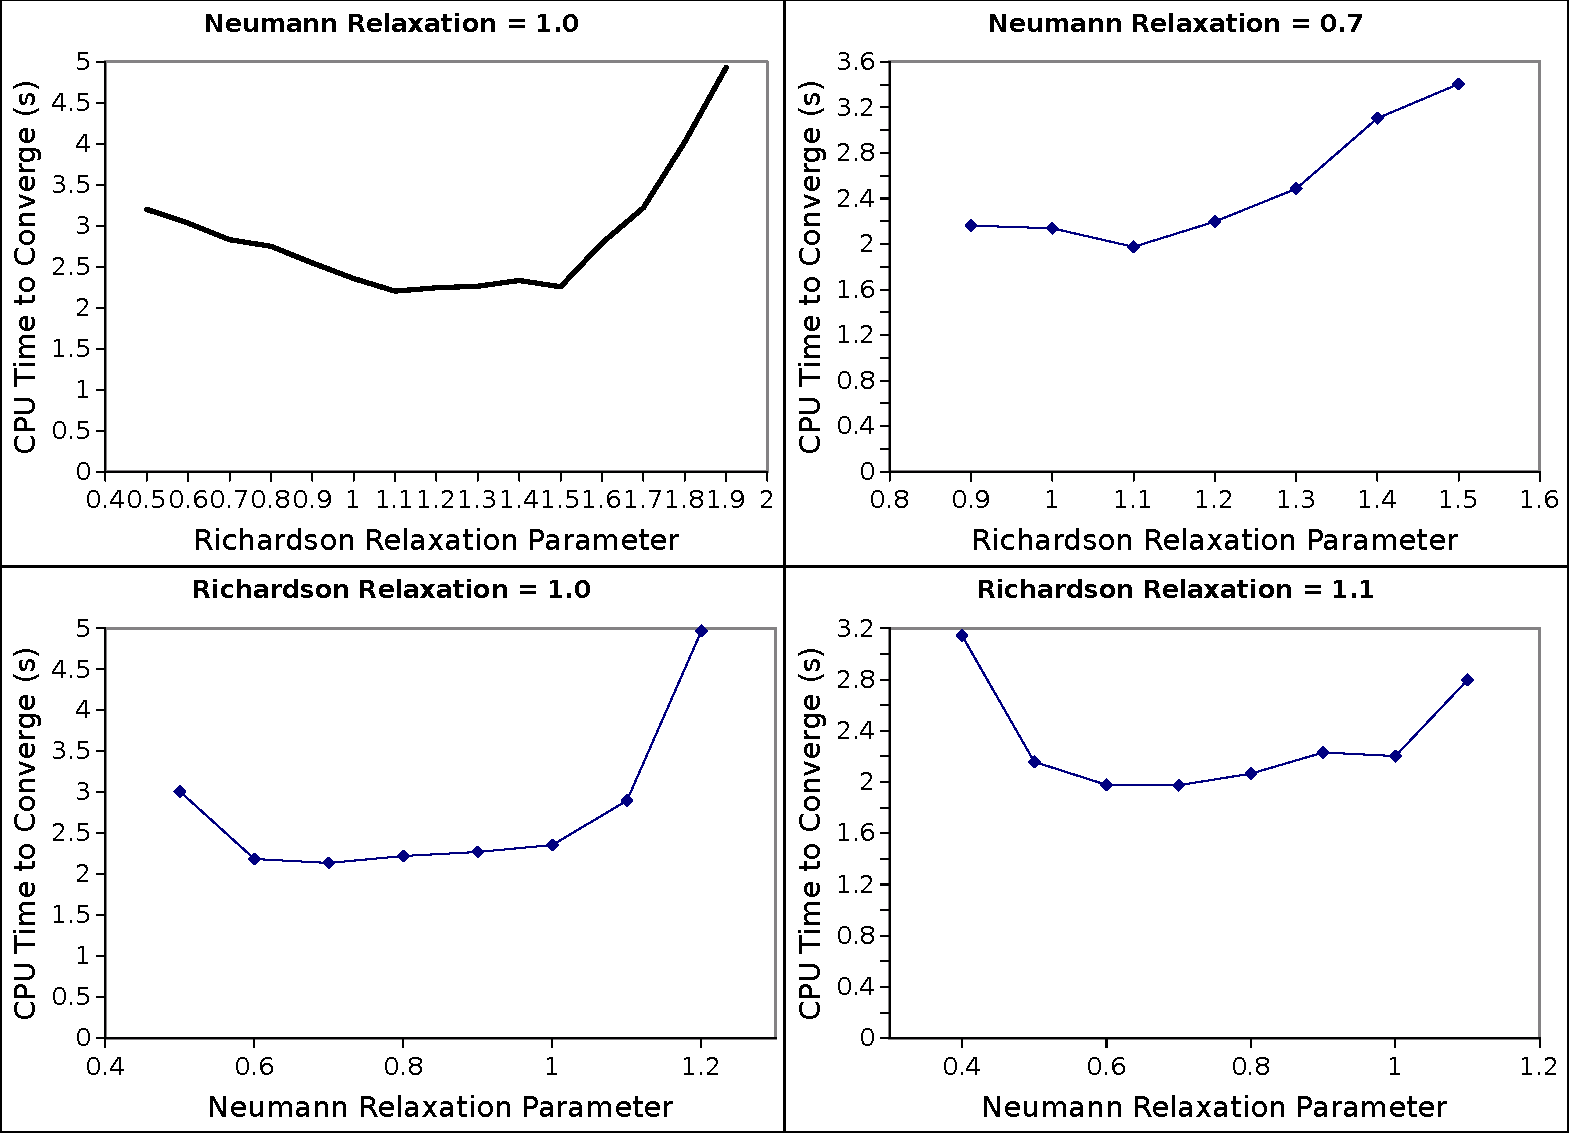
\includegraphics[width=6in]{chapters/spn_equations/relax_time.pdf}
  \end{center}
  \caption{\textbf{CPU time in seconds to converge a single eigenvalue
      iteration of the fuel assembly problem as a function of the
      relaxation parameters.} \textit{Starting in upper left and
      moving counter-clockwise: Neumann relaxation parameter fixed at
      1.0, Richardson relaxation parameter fixed at 1.0, Neumann
      relaxation parameter fixed at 0.7, Richardson relaxation
      parameter fixed at 1.1. For each calculation \sn{3}{4}
      stochastic histories were used to compute the MCSA correction at
      each iteration.}}
  \label{fig:relax_time}
\end{figure}

\clearpage

\subsection{Monte Carlo Estimator Comparison}
\label{subsec:spn_estimator_comparison}
With convergence obtained for the fuel assembly problem, the advanced
preconditioners will next be studied with both the collision and
expected value estimators using the best preconditioning and
relaxation parameter combinations found by the previous
analysis. Additionally, both the Richardson-based MCSA iteration given
by Eq~(\ref{eq:mcsa}) and the MINRES-based MCSA iteration given by
Eq~(\ref{eq:mcsa_minres}) will be used. Although the expected value
estimator achieved the best iterative performance in the previous
comparison and analysis for the simple Poisson problem in
\S~\ref{sec:parameter_estimator_analysis}, it is possible that the
collision estimator may perform better from a timing perspective due
to the sparsity lost by explicit preconditioning. The deterministic
component of the expected value estimator that couples the current
state to other local states through the iteration matrix stencil
requires application of the estimator to potentially several orders of
magnitude more states at every transition event.

For this study, the fuel assemby problem with a 1-group $SP_1$
discretization was solved using MCSA with the adjoint Monte Carlo
solver using both the collision and expected value estimators and both
the Richardson and MINRES fixed point iterations. Using the results
from the previous section, a Neumann relaxation parameter of 0.7 was
used with both estimators and fixed point iterations. For the
collision estimator, a Richardson relaxation parameter of 1.1 was used
with the Richardson iteration while it was found the expected value
estimator had the best performance when a Richardson relaxation
parameter of 1.0 was used instead. In addition, ILUT preconditioning
with a drop tolerance of \sn{1}{-5} and a fill level of 5 was used
with a reduced domain approximation fill level of 100 and a threshold
of \sn{1}{-10} as in the previous analysis. For each estimator, the
number of stochastic histories used to compute the MCSA correction was
varied from 25 to 50,000 with the number of MCSA iterations required
to converge to a tolerance of \sn{1}{-8} recorded for a single
eigenvalue iteration along with the CPU time required to achieve
convergence.

Figure~\ref{fig:spn_estimator_iters} gives the iteration count results
and Figure~\ref{fig:spn_estimator_time} gives the timing
results. Remarkably, although the fuel assembly problem is
significantly more complicated than the simple Poisson problem studied
in \S~\ref{sec:parameter_estimator_analysis}, the results here are
largely the same with Figure~\ref{fig:spn_estimator_iters} and
Figure~\ref{fig:estimator_nh_iters} having identical qualitative
behavior. Using the expected value estimator with both fixed point
iterations creates a relative insensitivity to the number of histories
used to compute the correction. Marginally better iterative and timing
performance was observed for the expected value estimator when using
the Richardson iteration. Better timing performance is expected as
computing the extrapolation parameter in the MINRES iteration requires
several additional parallel operations. However, we expect that
because the MINRES iteration will converge faster on its own when
compared to the Richardson iteration that better iterative performance
will be observed when it is accelerated with MCSA. The fact that this
was not observed signals that an MCSA scheme leveraging the expected
value estimator is also effectively insensitive to the fixed point
iteration used. For the collision estimator, the MINRES iteration
permits fewer stochastic histories to be used with each MCSA iteration
while still maintaining good iterative performance. With respect to
CPU time, there is a more pronounced effect due to the larger density
of states created by the explicit ILUT preconditioning. Using a
reduced domain fill level of 100 creates a situation where the
expected value estimator is significantly more expensive per history
to compute that the collision estimator due to the coupling of states.

\begin{figure}[t!]
  \begin{center}
    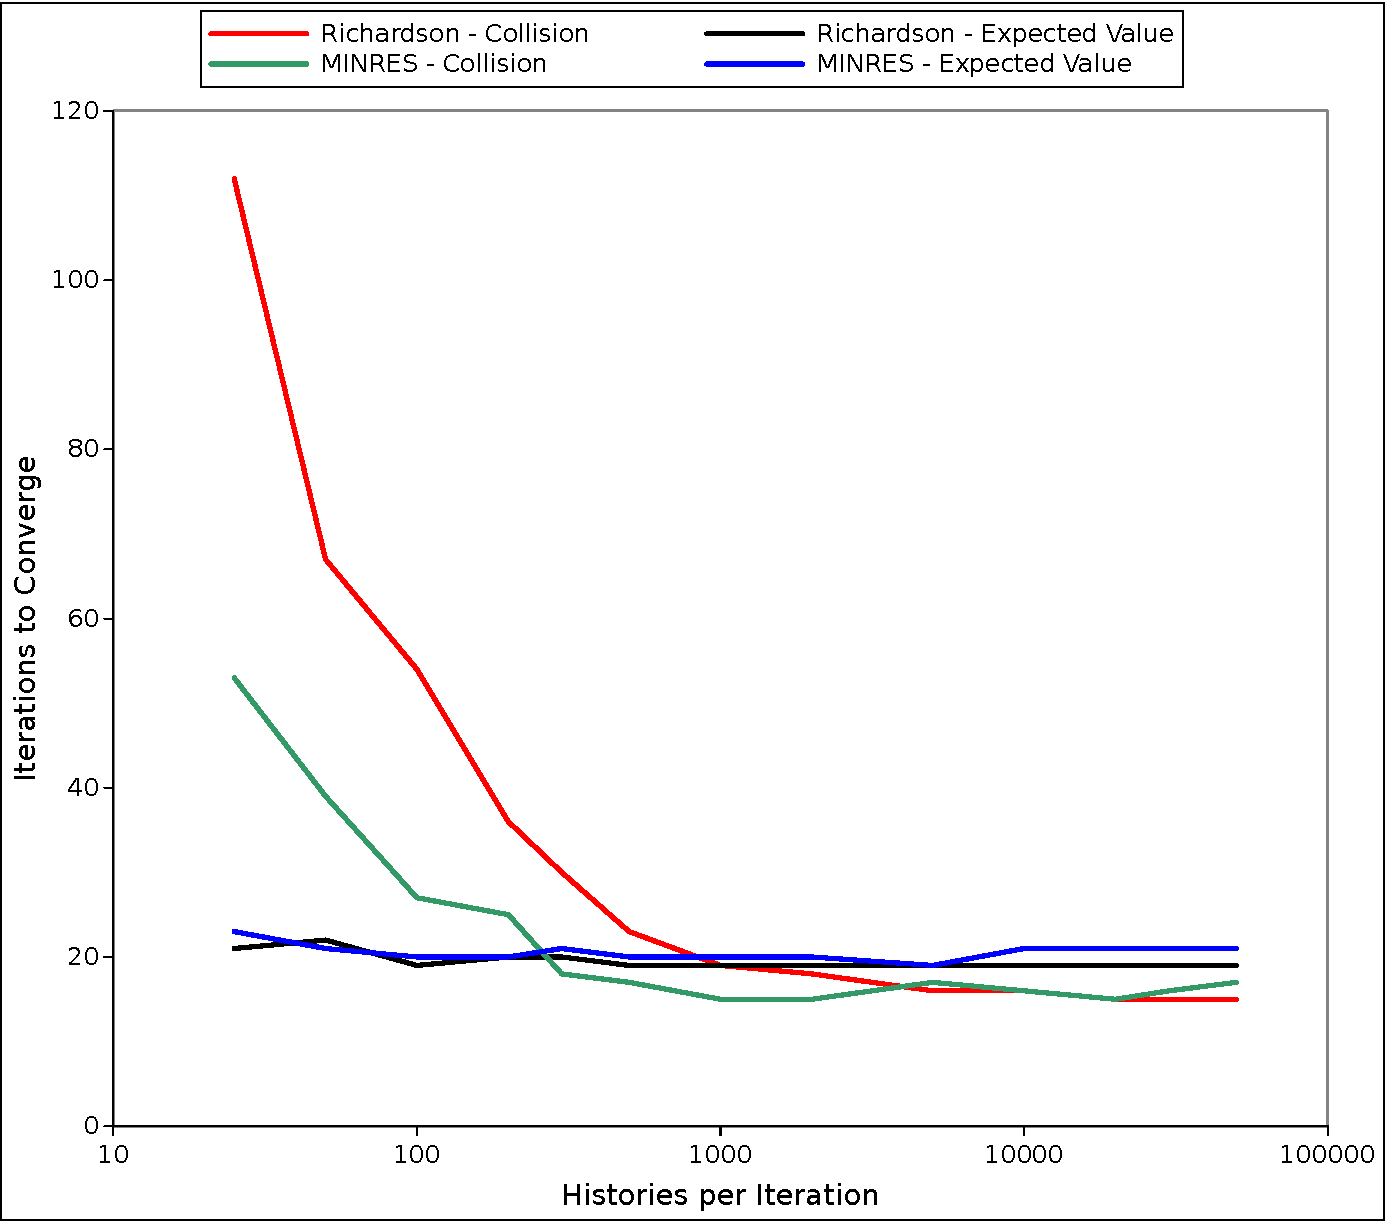
\includegraphics[width=6in]{chapters/spn_equations/estimator_iters.pdf}
  \end{center}
  \caption{\textbf{MCSA iterations required to converge the fuel
      assembly problem to a tolerance of \sn{1}{-8}.} \textit{Both the
      collision and expected value estimators were used with the
      adjoint Monte Carlo solver to compute the correction at each
      iteration. Each estimator was used with the Richardson and
      MINRES fixed point iterations within an MCSA iteration.}}
  \label{fig:spn_estimator_iters}
\end{figure}

\begin{figure}[t!]
  \begin{center}
    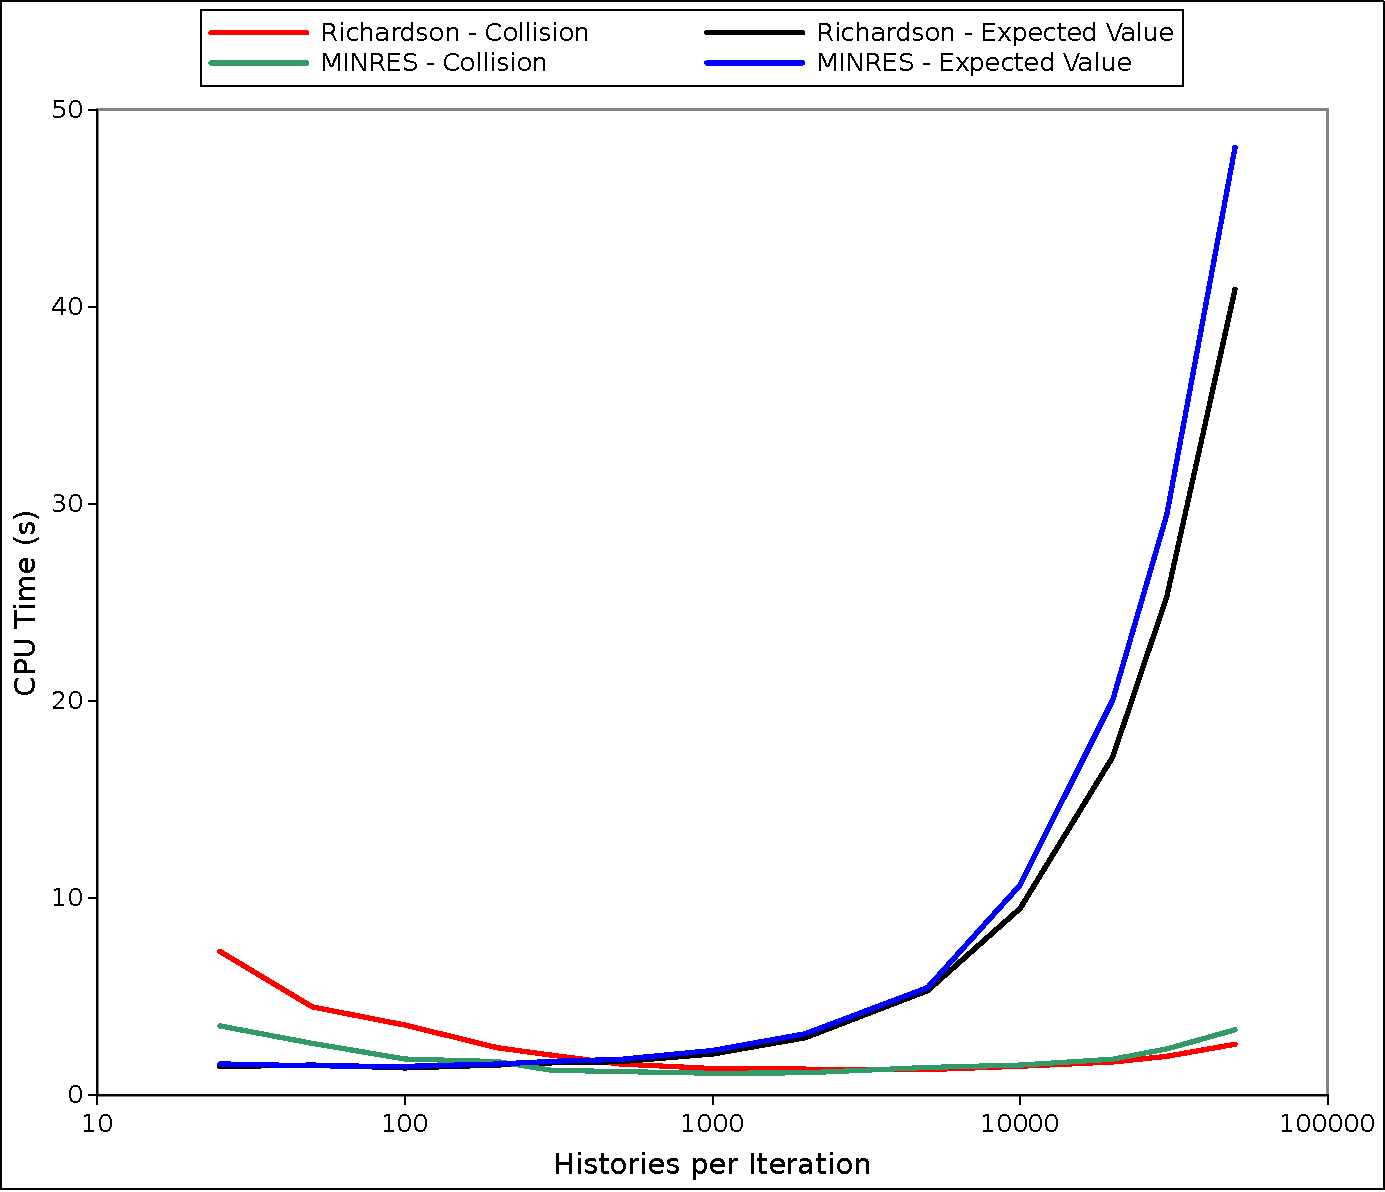
\includegraphics[width=6in]{chapters/spn_equations/estimator_time.pdf}
  \end{center}
  \caption{\textbf{Total CPU time in seconds required to converge the
      fuel assembly problem to a tolerance of \sn{1}{-8}.}
    \textit{Both the collision and expected value estimators were used
      with the adjoint Monte Carlo solver to compute the correction at
      each iteration. Each estimator was used with the Richardson and
      MINRES fixed point iterations within an MCSA iteration.}}
  \label{fig:spn_estimator_time}
\end{figure}

From both Figure~\ref{fig:spn_estimator_iters} and
Figure~\ref{fig:spn_estimator_time} we see that both estimators and
fixed point iterations have comparable iterative and timing
performance when 1,000 histories are used at each MCSA
iteration. Using 1,000 histories per MCSA iteration, the infinity norm
of the residual vector is presented at every MCSA iteration for both
estimators and both fixed point iterations in
Figure~\ref{fig:spn_estimator_convergence} as an additional means of
comparison. At this number of histories, all MCSA combinations
converge the fuel assembly problem monotonically at and approximately
the same rate, giving little reason to choose one over the other. The
end result is that both estimators provide a viable method for getting
good MCSA iterative performance with comparable timing
performance. For the collision estimator, using around 20,000
stochastic histories at every iteration gave the best iterative
performance while 500 histories per iteration gave the best iterative
performance when using the expected value estimator. For purely serial
computational performance, there is not a distinguishing feature for
the fuel assembly problem presented that would cause one to choose one
of the estimators and fixed point iterations over the other as they
all have similar minimum CPU times over the range of values tested.

\begin{figure}[t!]
  \begin{center}
    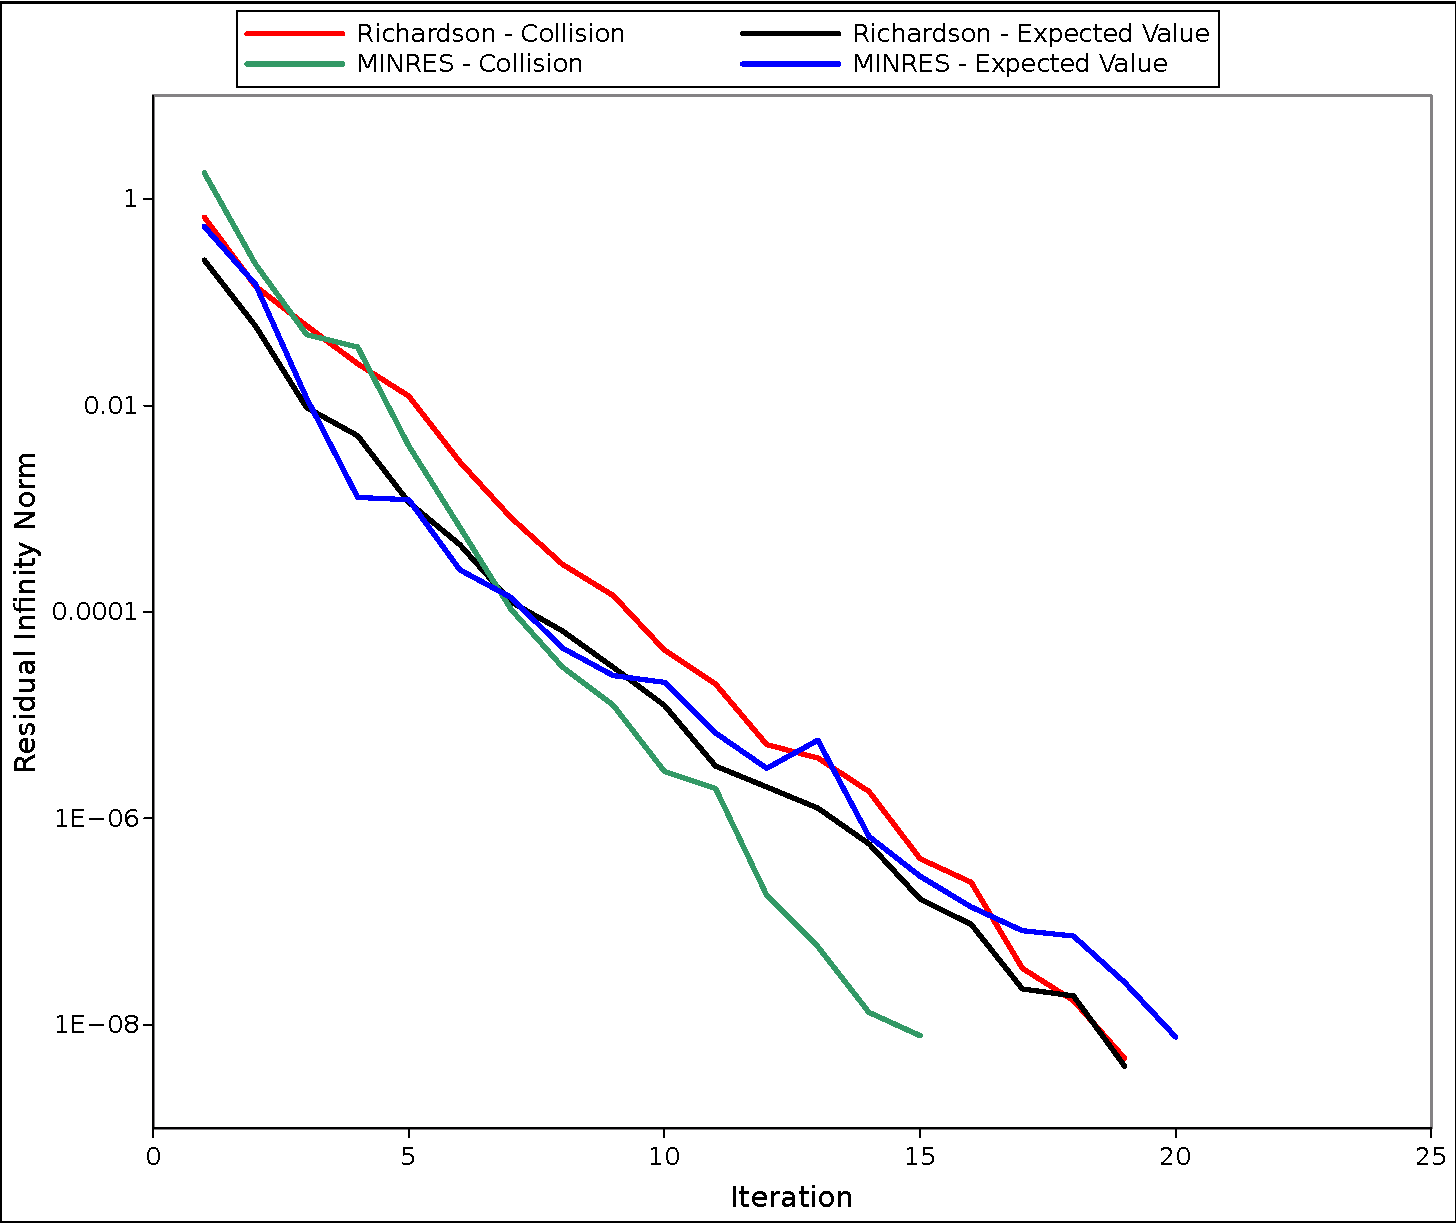
\includegraphics[width=6in]{chapters/spn_equations/estimator_convergence.pdf}
  \end{center}
  \caption{\textbf{Residual infinity norm as a function of MCSA
      iteration with 1,000 stochastic histories per iteration.}
    \textit{Both the collision and expected value estimators were used
      with the adjoint Monte Carlo solver to compute the correction at
      each iteration. Each estimator was used with the Richardson and
      MINRES fixed point iterations within an MCSA iteration.}}
  \label{fig:spn_estimator_convergence}
\end{figure}

\clearpage

%%---------------------------------------------------------------------------%%
\section{MCSA Verification}
\label{sec:spn_mcsa_verification}
Through the numerical studies presented in this chapter, we have
developed a set of preconditioning techniques that permit MCSA to be
used with the $SP_N$ form of the neutron transport equation and
applied to a difficult fuel assembly criticality problem. Along with
these preconditioning techniques, a set a varying MCSA parameters were
analyzed to find those that yielded the best performance for this
particular problem. In addition, several steps were taken to mitigate
the dense composite linear operators that arise when performing
explicit MCSA preconditioning in order to achieve convergence. Using
these results, we compare MCSA directly to conventional linear solvers
that would be typically used to solve the $SP_N$ form of the transport
equation as presented here. In particular, we will use a pair of
production Krylov solvers with which we will compare direct numerical
results in order to verify MCSA solutions in this section and
iterative and CPU timing performance in the next order to gauge
feasibility and identify areas that require further research.

In order to verify the correctness of the MCSA method and
implementation used for this work, MCSA solutions to the fuel assembly
problem with 1, 2, and 4 energy groups using $SP_1$ discretization
will be directly compared over all group and cell fluxes computed by
converging the criticality problem using both BiCGStab and GMRES
production implementations from the Trilinos scientific computing
library Aztec \citep{heroux_overview_2005}. In addition to comparing
the cell and group fluxes, the number of eigenvalue iterations
required to converge the problem along with the eigenvalue itself will
be compared as a means of verification. If all values computed using
MCSA agree with the results from the production Krylov solvers within
the solution tolerance then the MCSA solutions will be deemed verified
for these problems. Additionaly, this verification is only applicable
to serial results with parallel verification for this problem provided
in Chapter~\ref{ch:parallel_methods}.

For the verification calculations, all solvers will be preconditioned
with ILUT using a drop tolerance of \sn{1}{-5} and a fill level of
5. For GMRES, no restrictions were placed on the size of the subspace
and therefore no restarts occurred. When the collision estimator was
used with MCSA, \sn{2}{4} stochastic histories were used to compute
the correction for every energy group in the problem (\sn{4}{4} and
\sn{8}{4} histories total for the 2 and 4 group calculations
respectively) corresponding to approximately 1 stochastic history per
DOF. When the expected value estimator was used, \sn{5}{2} stochastic
histories used for each energy group (\sn{1}{3} and \sn{1.5}{3}
histories total for the 2 and 4 group calculations) giving
approximately 1 stochastic history for every 5 DOFs. The reduced
domain approximation was also applied in conjuction with the ILUT
preconditioning using a fill level of 100 and a threshold value of
\sn{1}{-10} to reduce the density of states in the Monte Carlo
problem. For relaxation parameters, all MCSA compuations used a
Neumann relaxation parameter of 0.7 while a Richardson relaxation of
1.1 was used with the collision estimator and 1.0 with the expected
value estimator as determined by the previous analysis of the
relaxation parameters. Table~\ref{tab:spn_solver_defs} gives
definitions for the solvers used to generate the results in the
remainder of this section. For the energy group structures,
Table~\ref{tab:spn_group_structure} gives the lower bounds of each
group in eV (an implicit upper bound of \sn{2}{6} eV is assumed for
group 0).
\begin{table}[h!]
  \begin{center}
    \begin{tabular}{ll}\hline\hline
      \multicolumn{1}{l}{\textbf{Name}} & 
      \multicolumn{1}{l}{\textbf{Definition}} \\
      BiCGStab-ILUT & BiCGStab preconditioned with ILUT \\
      GMRES-ILUT & GMRES preconditioned with ILUT \\
      MCSA-ILUT-R-C & MCSA preconditioned with ILUT using Richardson \\ 
                    & fixed point iteration and collision estimator \\
      MCSA-ILUT-MR-C & MCSA preconditioned with ILUT using MINRES \\
                     & fixed point iteration and collision estimator \\
      MCSA-ILUT-R-EV & MCSA preconditioned with ILUT using Richardson \\
                     & fixed point iteration and expected value estimator \\
      MCSA-ILUT-MR-EV & MCSA preconditioned with ILUT using MINRES \\
                      & fixed point iteration and expected value estimator \\
      %%
      \hline\hline
    \end{tabular}
  \end{center}
  \caption{\textbf{Solver definitions used for MCSA verification and
      performance analysis.} \textit{The ILUT preconditioner
      parameters were identical for all calculations and solvers.}}
  \label{tab:spn_solver_defs}
\end{table}
\begin{table}[h!]
  \begin{center}
    \begin{tabular}{cl}\hline\hline
      \multicolumn{1}{c}{\textbf{Number of Groups}} & 
      \multicolumn{1}{l}{\textbf{Lower Bounds (eV)}} \\
      1 & \{ \sn{1}{-5} \} \\
      2 & \{ \sn{1}{-1}, \sn{1}{-5} \} \\
      4 & \{ \sn{1}{1}, \sn{1}{0}, \sn{1}{-1}, \sn{1}{-5} \} \\
      %%
      \hline\hline
    \end{tabular}
  \end{center}
  \caption{\textbf{Energy group lower bounds for the multigroup fuel
      assembly criticality problem in electron volts.} \textit{An
      implicit upper bound of \sn{2}{6} eV is assumedfor group zero.}}
  \label{tab:spn_group_structure}
\end{table}

For every combination of energy group structure and solver, the
eigenvalue problem was converged with an eigensolver tolerance of
\sn{1}{-6} and a linear solver tolerance of \sn{1}{-8} in a serial
calculation. Table~\ref{tab:serial_ev_results} gives the eigenvalue
computed by each solver for each problem as well as the number of
eigenvalue iterations required to converge. For every problem, each
solver converged to the same eigenvalue within the tolerance of the
eigensolver in the same number of eigenvalue iterations.
\begin{table}[h!]
  \begin{center}
    \begin{tabular}{lccc}\hline\hline
      \multicolumn{1}{c}{\textbf{Solver}} & 
      \multicolumn{1}{c}{\textbf{Number of Groups}} & 
      \multicolumn{1}{c}{\textbf{Iterations}} &
      \multicolumn{1}{c}{\textbf{Eigenvalue}} \\
      \hline
      BiCGStab-ILUT & 1 & 25 & 1.1059870 \\
      GMRES-ILUT & 1 & 25 & 1.1059870 \\
      MCSA-ILUT-R-C & 1 & 25 & 1.1059870 \\
      MCSA-ILUT-MR-C & 1 & 25 & 1.1059870 \\
      MCSA-ILUT-R-EV & 1 & 25 & 1.1059870 \\
      MCSA-ILUT-MR-EV & 1 & 25 & 1.1059870 \\
      \hline
      BiCGStab-ILUT & 2 & 35 & 1.1552390 \\
      GMRES-ILUT & 2 & 35 & 1.1552390 \\
      MCSA-ILUT-R-C & 2 & 35 & 1.1552390 \\
      MCSA-ILUT-MR-C & 2 & 35 & 1.1552390 \\
      MCSA-ILUT-R-EV & 2 & 35 & 1.1552390 \\
      MCSA-ILUT-MR-EV & 2 & 35 & 1.1552390 \\
      \hline
      BiCGStab-ILUT & 4 & 31 & 1.1758500 \\
      GMRES-ILUT & 4 & 31 & 1.1758500 \\
      MCSA-ILUT-R-C & 4 & 31 & 1.1758500 \\
      MCSA-ILUT-MR-C & 4 & 31 & 1.1758500 \\
      MCSA-ILUT-R-EV & 4 & 31 & 1.1758500 \\
      MCSA-ILUT-MR-EV & 4 & 31 & 1.1758500 \\
      %%
      \hline\hline
    \end{tabular}
  \end{center}
  \caption{\textbf{Serial eigensolver verification results for the
      fuel assembly problem.} \textit{Each calculation was converged
      with the same eigensolver and linear solver tolerances.}}
  \label{tab:serial_ev_results}
\end{table}

For each converged eigenvalue calculation, the scalar flux in each
energy group was compared over the entire spatial with the
BiCGStab-ILUT solution used as the reference to compute an absolute
difference. For the 1 group calculations, these absolute differences
are plotted spatially along the centerline of the fuel assembly in
Figure~\ref{fig:serial_1_group_diff}. Interestingly, except for the
MCSA-ILUT-MR-C calculation, all other 1-group calculations including
GMRES had a maximum global flux difference of \sn{9.313}{-10} even
though different spatial results were observed. For the MCSA-ILUT-MR-C
calculation, a slightly larger maximum error of \sn{2.205}{-9} was
observed for reasons that remain unexplained. All 1-group calculations
have a minimum observed absolute difference of 0 with respect to the
BiCGStab calculation.

\begin{figure}[t!]
  \begin{center}
    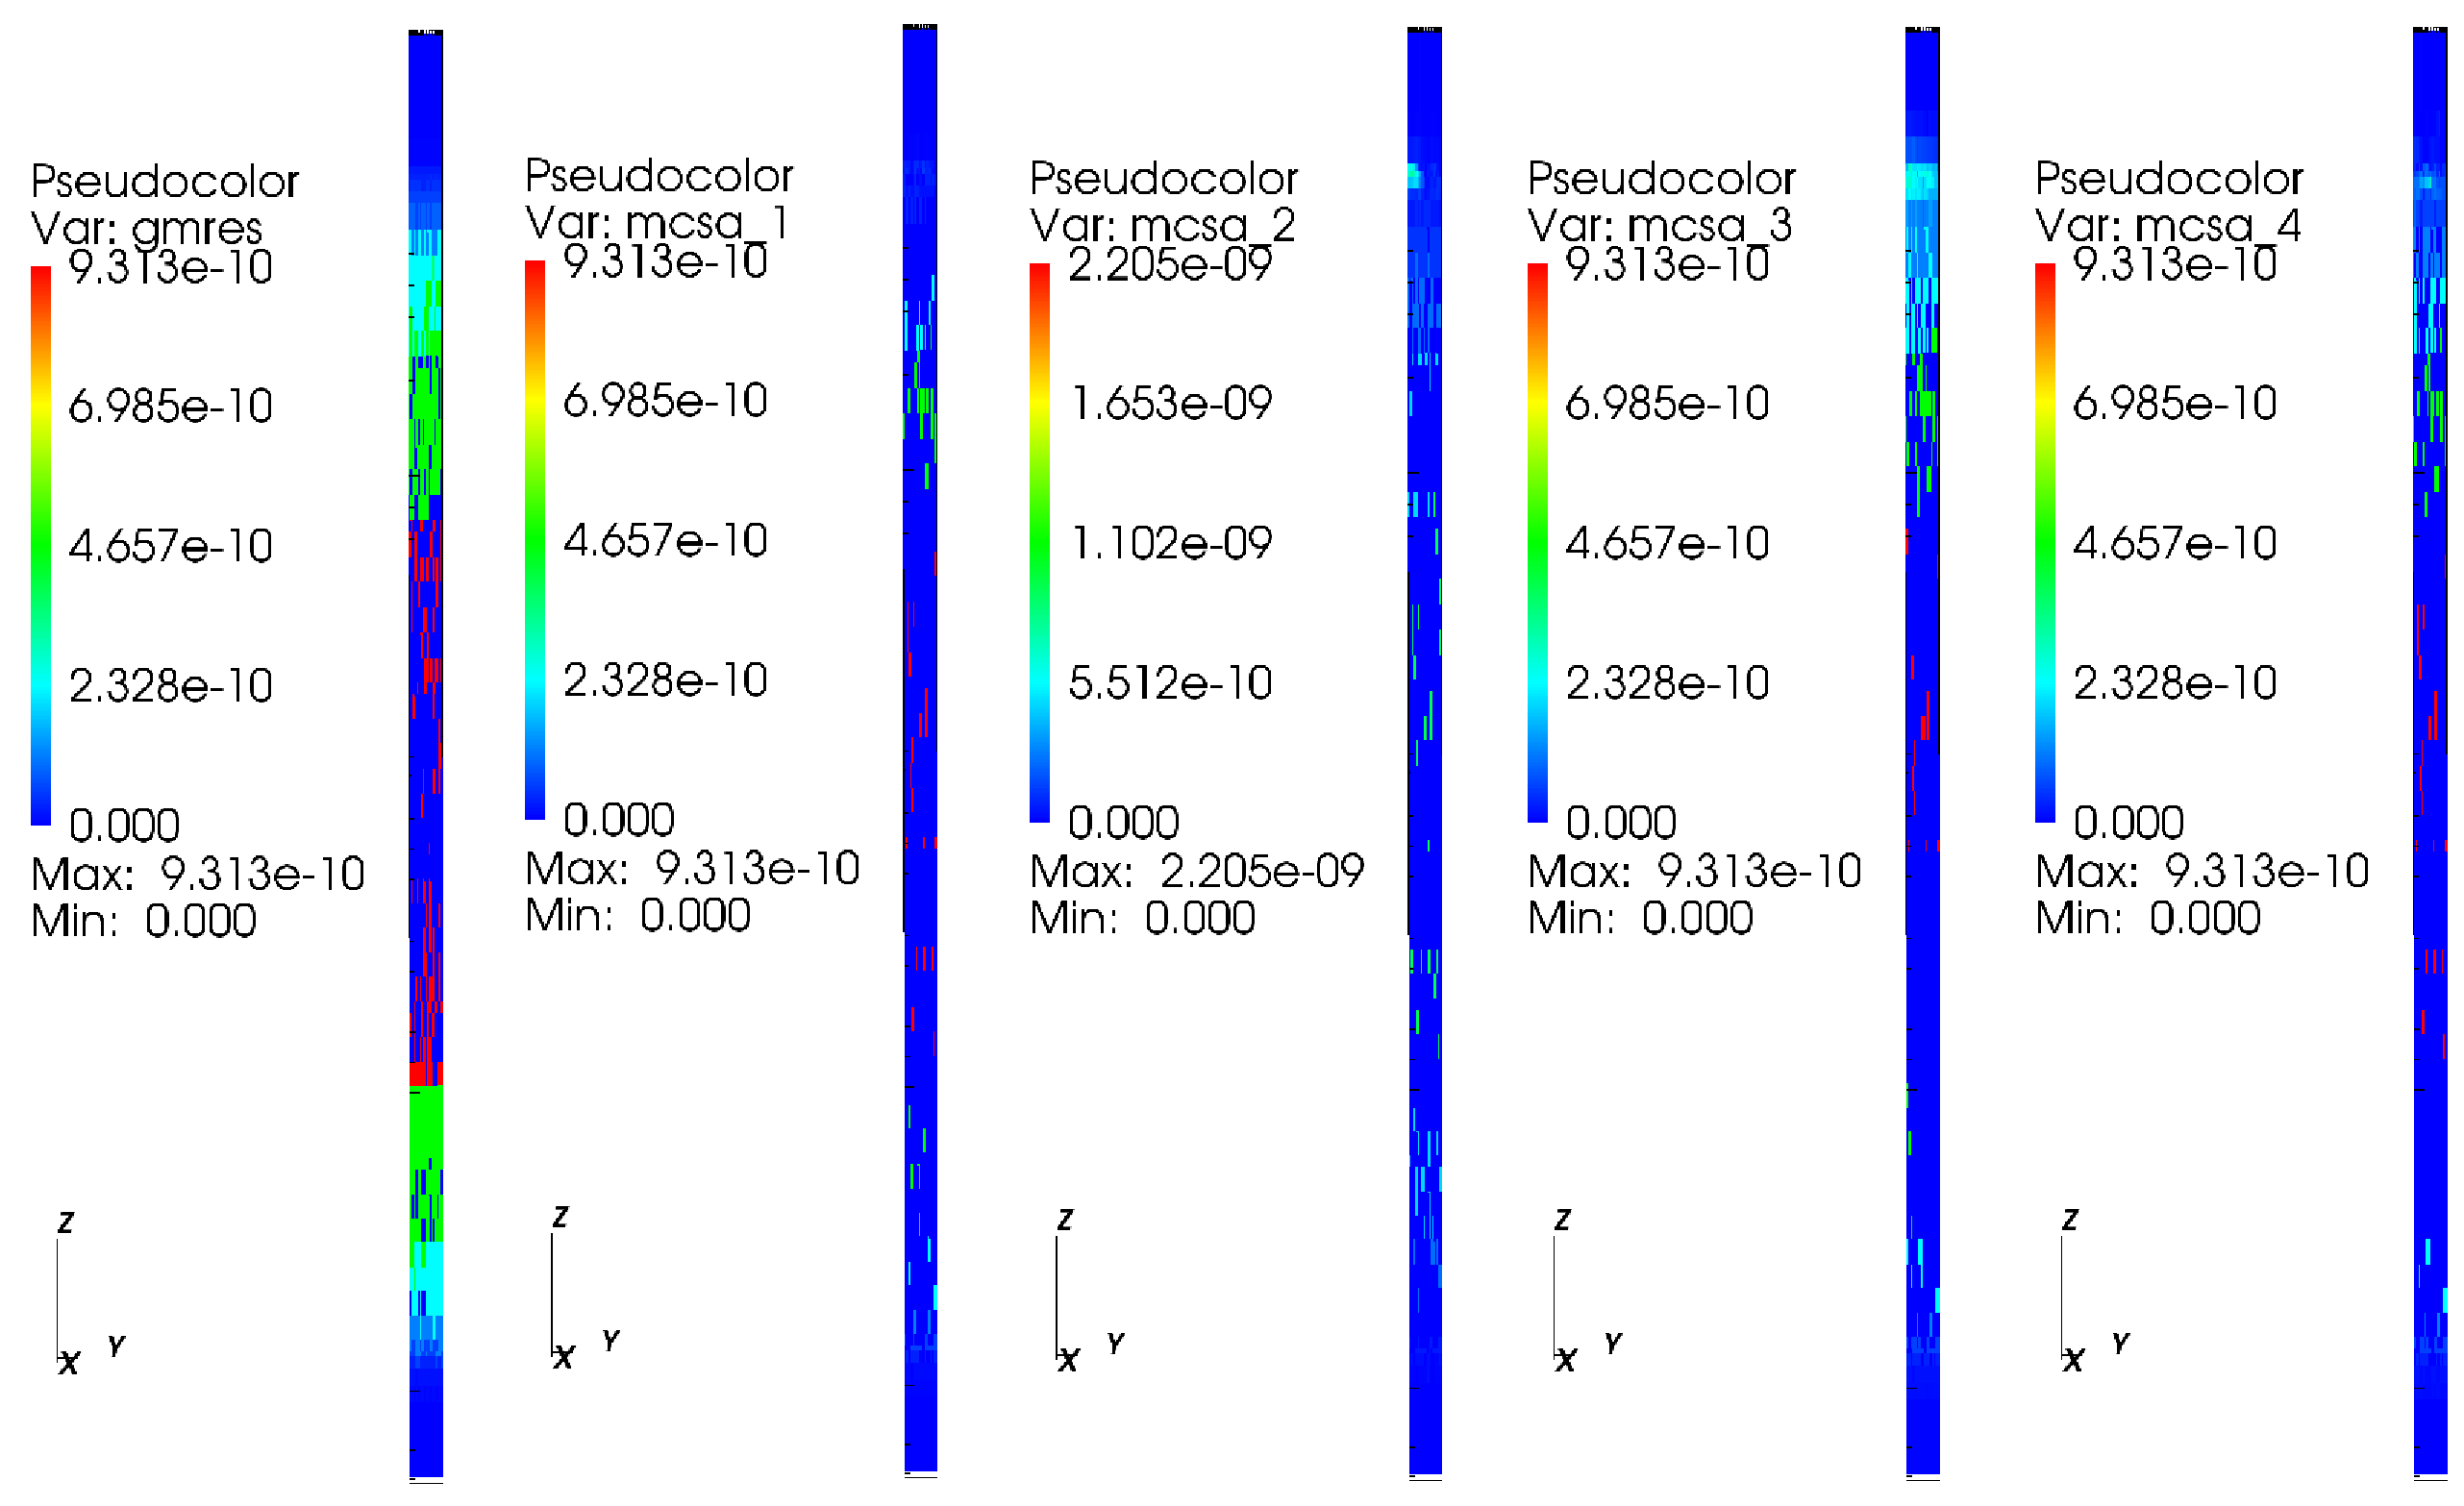
\includegraphics[width=6in]{chapters/spn_equations/serial_1_group.pdf}
  \end{center}
  \caption{\textbf{Absolute difference of the group 0 scalar flux
      between the Aztec BiCGStab calculations and Aztec GMRES and the
      MCSA variations for the 1-group calculation.} \textit{Left to
      right: GMRES-ILUT, MCSA-ILUT-R-C, MCSA-ILUT-MR-C,
      MCSA-ILUT-R-EV, MCSA-ILUT-MR-EV.}}
  \label{fig:serial_1_group_diff}
\end{figure}

Table~\ref{tab:serial_differences} gives the maximum and minimum
absolute differences for all calculations and all energy groups using
the BiCGStab calculation as the reference. All comparisons were
performed within a group such that the MCSA-ILUT-R-C results in group
3 for the 4-group calculation were computed with the BiCGStab-ILUT
solution in group 3 for the 4-group calculation as a reference.

%%---------------------------------------------------------------------------%%
\section{MCSA Performance Comparison to Conventional Methods}
\label{sec:spn_comparison}
Using the same set of solver parameters used for verification, MCSA
will be directly compared to the production Krylov solvers in terms of
both iterative performance and CPU timing for solutions to the fuel
assembly problem. In addition to the parameters used for the
verification analysis, artificial absorption was also introduced with
a value of 0.2 for the MCSA calculations that used the collision
esitmator as CPU timing performance was improved without a loss in
iterative performance. Adding this absorption did not change the
numerical results of the calculation.

Figure~\ref{fig:spn_comparison_iterations} gives the average number of
linear solver iterations required to converge a single eigenvalue
iteration of the fuel assembly problem as a function of the number of
energy groups. In general, the iterative performance of all the
solvers tested is comparable with BiCGStab performing the best. We
expect this because not only are the multigroup $SP_N$ equations
elliptic and positive-definite, but they are also nearly symmetric and
therefore we expect the conjugate gradient-based methods to perform
well. It also important to note that the iterative performance of each
solver is not a strong function of the number of energy groups in the
problem (and therefore the problem size). For MCSA, we are linearly
increasing the number of stochastic histories used to compute the
correction at each iteration as the number of energy groups are
increased and therefore the work performed for the problem is of
$O(N)$. It is also important to note the the reduced domain
approximation parameters, particularly the fill level, were fixed as
the number of energy groups was increased. By fixing the fill level,
we are effectively fixing the amount of information contained in the
composite linear operator available for the Monte Carlo
problem. Limiting this information to 100 entries per row in the
preconditioned system did not appear to have a significant effect on
the iterative performance of the solver. For larger numbers of energy
groups (and therefore DOFs) this may be an issue and this number may
need to be increased to maintain iterative performance. Currently,
memory restrictions arising from the explicit preconditioning strategy
prevent larger energy groups to be analyzed using an appropriate
preconditioner for the fuel assembly problem.

\begin{figure}[t!]
  \begin{center}
    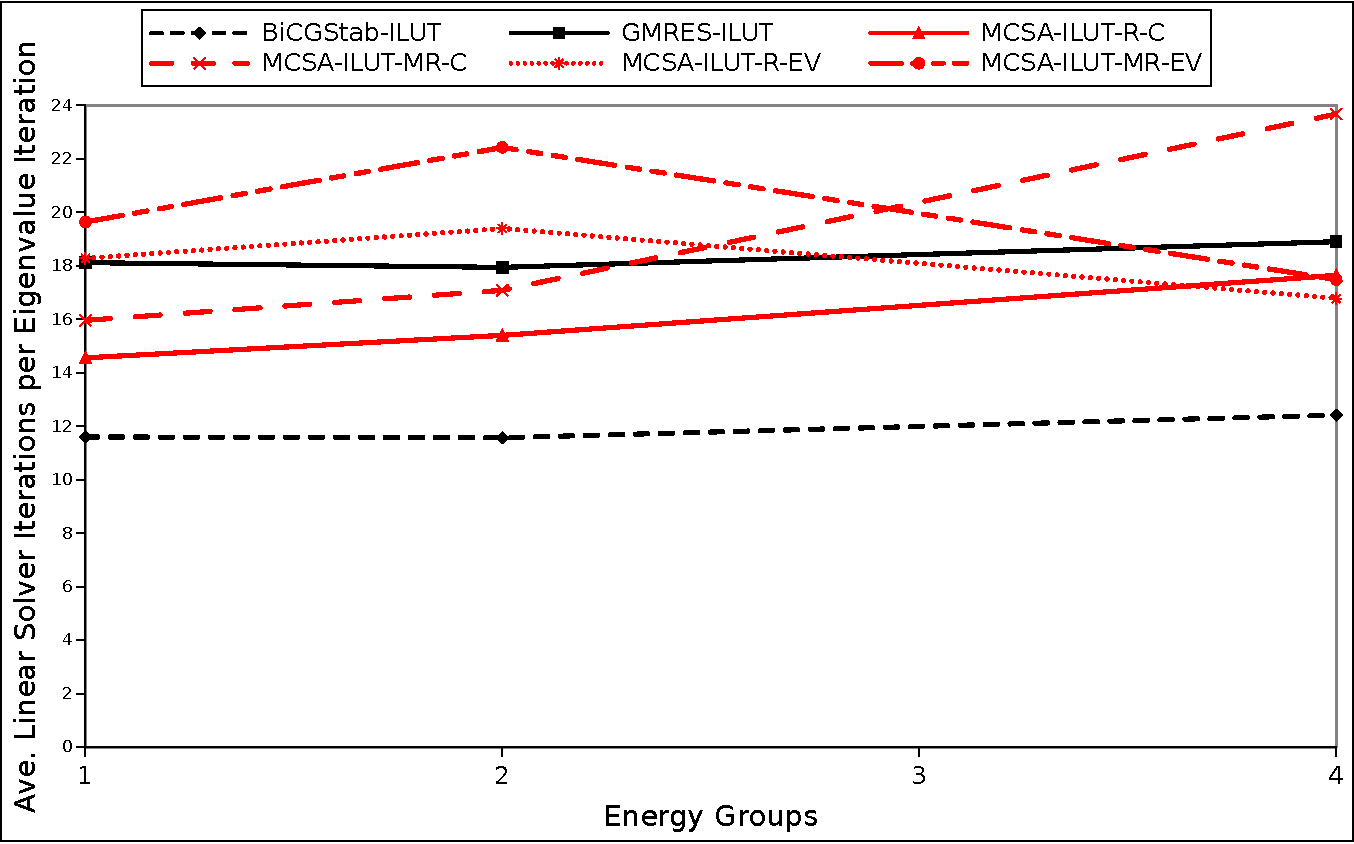
\includegraphics[width=6in]{chapters/spn_equations/solver_iters.pdf}
  \end{center}
  \caption{\textbf{Average number of iterations required to converge
      each eigenvalue iteration for the fuel assembly problem as a
      function of energy groups.}
    \textit{Table~\ref{tab:spn_solver_defs} gives the description for
      each solver type presented in the legend.}}
  \label{fig:spn_comparison_iterations}
\end{figure}

Although iterative performance for MCSA was comparable to that
observed for production Krylov implementations using exactly the same
preconditioning scheme, timing performance is not as
comparable. Figure~\ref{fig:spn_comparison_time} gives the average CPU
time per linear solver iteration required to converge the fuel
assembly problem with all linear solver iterations over all eigenvalue
iterations used to compute the average. The production Krylov solver
implementations are approximately an order of magnitude faster than
the MCSA implementations presented here. We expect these results for
several reasons. First, even when the reduced domain approximation is
used there are $O(100)$ elements in each row of the system and each of
those elements must be processed during a transition in the Monte
Carlo random walk sequence. In addition, although the preconditioned
fixed point iterations used in the MCSA sequence do not use the
composite linear operator but rather a sequence of matrix vector
multiplies to achieve the same preconditioning effect, they do use the
explicitly extracted inverse of the preconditioning matrices which
themselves are dense, leading to exceedingly slow computation times
even in the fixed point iteration. For the production Krylov methods,
the ILUT preconditioners are applied to a vector with two triangular
solves, one for each triangular factor. Also, the original linear
operator has $O(10)$ elements in each row of the system, an order of
magnitude less than that used in the reduced domain composite
operator. Second, the implementation presented here has not been
optimized and it is likely that several components of the algorithm
can be implemented in a more desireable time complexity. The
production Krylov solvers presented here have enjoyed decades of
professional development and optimization. However, it is most
important to note here that the CPU timing data presented in
Figure~\ref{fig:spn_comparison_time} shows that all methods have the
same time complexity; their differences are merely the manifestation
of a large time constant due to the effects of the explicit
preconditioning scheme. For transport systems where this is not a
problem, the literature explicitly shows that MCSA can be competetive
with these production Krylov methods using CPU time as a measure
\citep{evans_monte_2012}.

\begin{figure}[t!]
  \begin{center}
    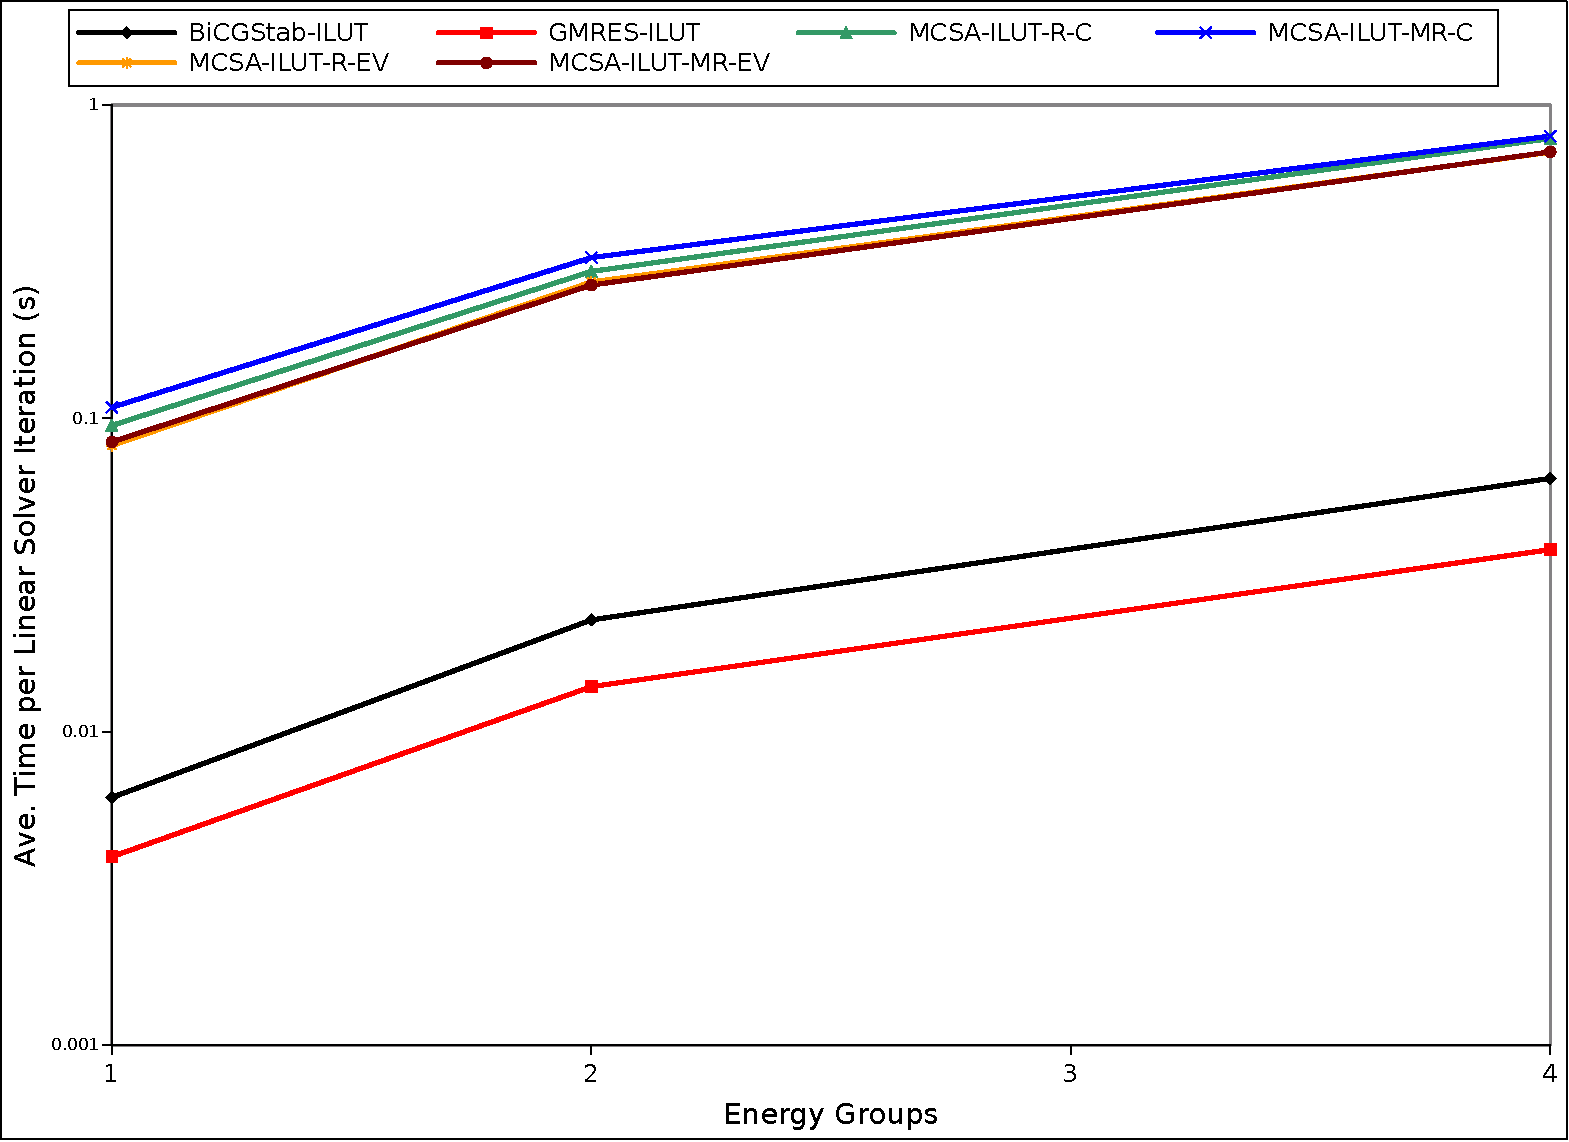
\includegraphics[width=6in]{chapters/spn_equations/solver_time.pdf}
  \end{center}
  \caption{\textbf{Average CPU time per linear solver iteration in
      seconds for the fuel assembly problem as a function of energy
      groups.}  \textit{All linear solver iterations over all
      eigenvalue iterations were used to compute the
      average. Table~\ref{tab:spn_solver_defs} gives the description
      for each solver type presented in the legend.}}
  \label{fig:spn_comparison_time}
\end{figure}

Finally, not considered in Figure~\ref{fig:spn_comparison_time} is the
time required to actually form the explicit inverse preconditioner
matrices and the composite operator through matrix-matrix
multiplication. The timing numbers reported were simply to perform the
MCSA iteration procedure with the composite operator already
formed. Figure~\ref{fig:spn_comparison_prec_time} additionally
presents the CPU times for MCSA convergence with the time to form the
inverse of the preconditioners and the composite linear operator
through matrix-matrix multiplication amortized over all iterations. As
is readily observed, including the costs of these operations increases
the MCSA computation time by another order of magnitude.

\begin{figure}[t!]
  \begin{center}
    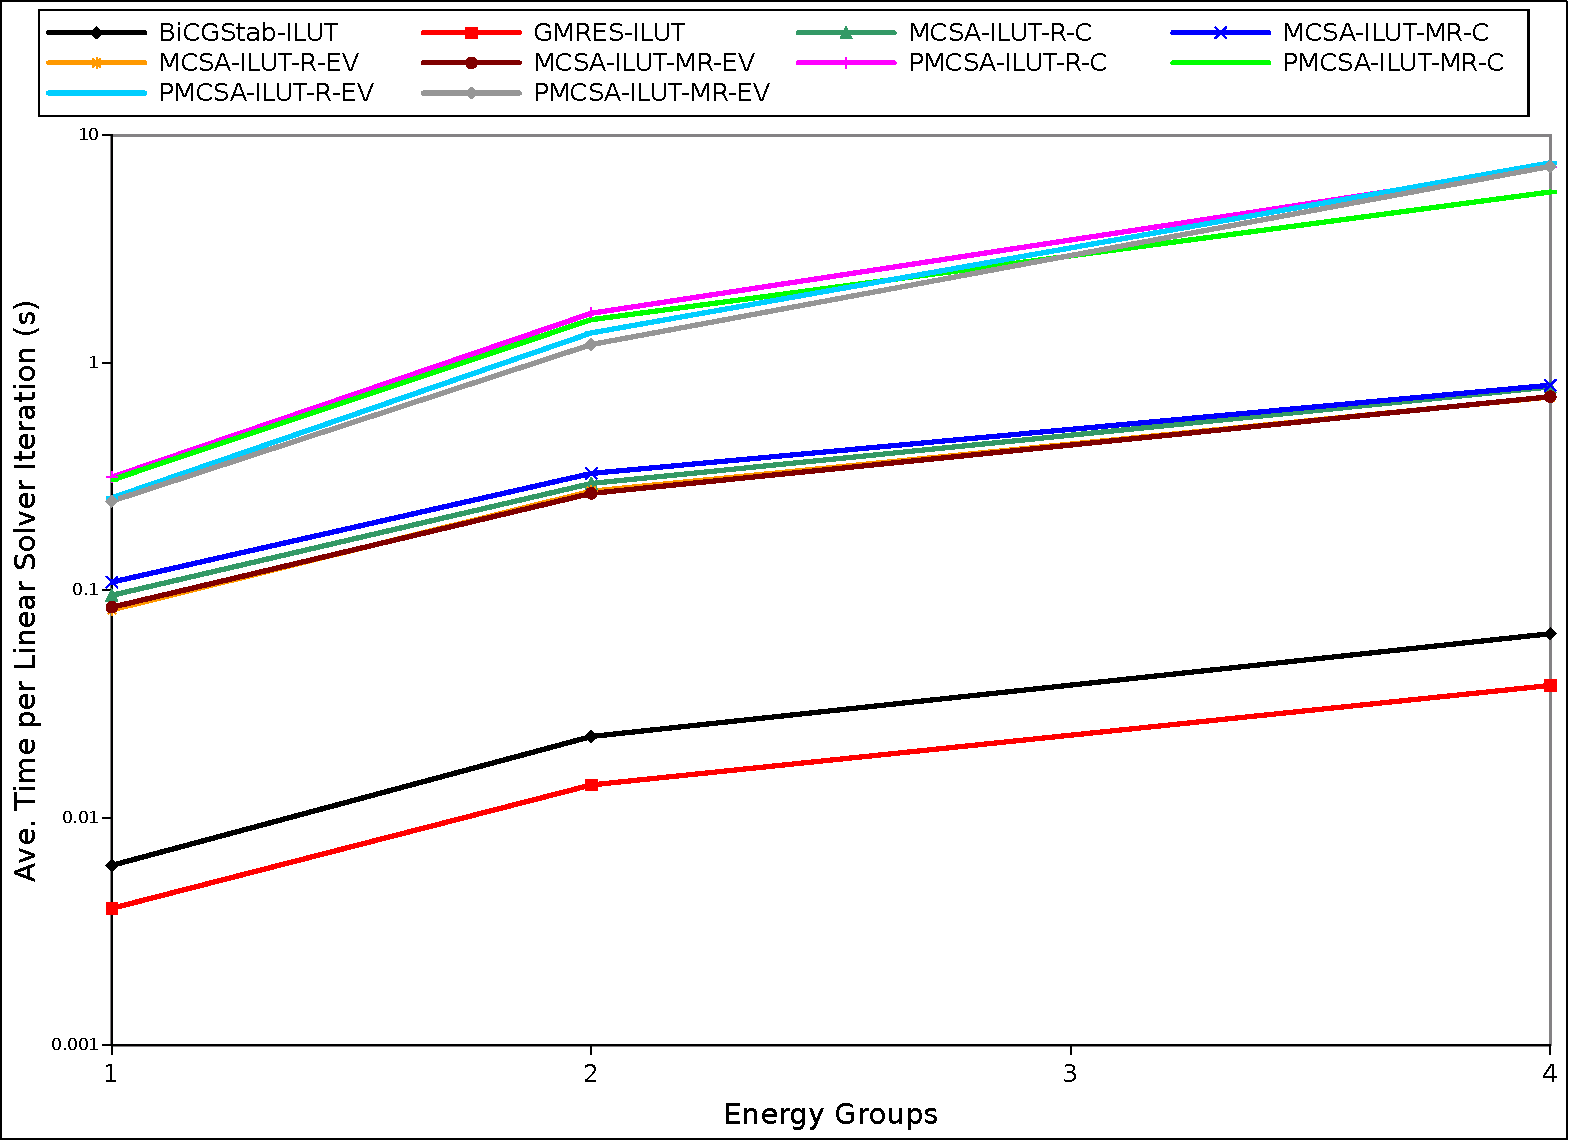
\includegraphics[width=6in]{chapters/spn_equations/solver_p_time.pdf}
  \end{center}
  \caption{\textbf{Average CPU time per iteration in seconds for the
      fuel assembly problem as a function of energy groups with
      preconditioning time included for the MCSA methods.}
    \textit{All linear solver iterations over all eigenvalue
      iterations were used to compute the
      average. Table~\ref{tab:spn_solver_defs} gives the description
      for each solver type presented in the legend. Data labeled
      starting with PMCSA is identical to those labeled with MCSA
      except that they additionally include the cost of generating the
      inverse of the preconditioners and composite linear operator.}}
  \label{fig:spn_comparison_prec_time}
\end{figure}

Based on the performance results in this section, MCSA shows promise
as a competitive and perhaps even superior method for solutions to the
neutron transport problem discretized with the $SP_N$
approximation. Not only are the correct answers produced when compared
to production linear solvers, but the iterative performance is
comparable to production Krylov methods with identical preconditioning
that would typically be used every-day calculations. From a CPU timing
perspective, the methods yield the same time complexity as a function
of the number of energy groups in the problem when compared to the
production Krylov methods. Here, a large time constant is generated
due to the explicit preconditioning strategy and the generation of
dense linear operators as a result. To improve these results and put
general MCSA schemes into a performance regime where they are
competitive with Krylov methods for neutron transport problems,
significant research will be required to improve upon the explicit
preconditioning scheme presented here.
